%! TEX root = ./thesis.tex
\chapter{Einleitung}

Diese Arbeit beschäftigt sich mit algorithmischen Suchproblemen. 
Hierbei ist eine Eingabeinstanz gegeben für welche eine entsprechende Lösung gesucht wird.
Beispiele für solche Suchprobleme sind:
\begin{enumerate}[label=\arabic*.,beginpenalty=0,midpenalty=0]
    \item Gegeben eine positive Zahl $n$, berechne die Primfaktorzerlegung von $n$.
    \item Sei $G$ eine kontextfreie Grammatik. Gegeben ein Wort $w$, berechne einen Ableitungsbaum von $w$ über $G$ an, oder gebe sonst „$w$ nicht von $G$ generiert“ aus.
    \item Gegeben ein Graph, berechne das größte Matching in diesem Graphen.
    \item Gegeben ein Graph, berechne eine Knotenfärbung mit drei Farben, oder gebe sonst „nicht färbbar mit drei Farben“ aus.
    \item Gegeben ein Graph, berechne eine größte Clique in diesem Graphen.
    \item Gegeben ein Graph und eine positive Zahl $k$, berechne eine Clique mit $\geq k$ Knoten in diesem Graphen, oder gebe sonst „keine Clique mit $k$ Knoten möglich“ aus.
    \item Gegeben eine aussagenlogische Formel $\phi$, bestimme eine erfüllende Belegung für $\phi$, oder gebe sonst „unerfüllbar“ aus.
    \item Gegeben eine aussagenlogische Formel $\phi$, bestimme einen Beweis (unter einem geeigneten Beweissystem, z.B. Resolution) für die Gültigkeit von $\phi$, oder gebe sonst eine Belegung an, welche $\phi$ nicht erfüllt.
    \item Gegeben eine prädikatenlogischen Satz $\phi$ in der Sprache der Arithmetik\sidenote{Gemeint ist die prädikatenlogische Sprache mit einer Konstante $0$, einer unären Nachfolgerfunktion, je binären Funktionen $+$, $\times$, und binärer Relation $\leq$.}, bestimme einen Beweis (unter einem geeigneten vollständigem Kalkül, z.B. Sequenzenkalkül) für die Gültigkeit von $\phi$ ($\phi$ ist wahr in jeder Struktur), oder gebe sonst „$\phi$ ungültig“ aus.
\end{enumerate}
Innerhalb des Forschungsbereichs der theoretischen Informatik beschäftigt sich die Berechenbarkeitstheorie mit der Frage, welche dieser Aufgaben überhaupt algorithmisch berechenbar sind. Das Beispiel (9) ist z.B. überhaupt nicht berechenbar, in dem Sinn dass kein Algorithmus existiert, welcher für jeden Satz $\phi$ nach endlicher Zeit mit der korrekten Lösung antwortet.
Alle anderen Probleme (1)--(8) sind im Prinzip algorithmisch lösbar, indem alle möglichen Lösungsmöglichkeiten durchsucht werden.

Der Unterbereich der algorithmischen Komplexitätstheorie ist weniger an den prinzipiellen Grenzen von Berechenbarkeit interessiert, sondern fokussiert sich unter den berechenbaren Aufgaben damit, welche Ressourcen (Rechenzeit, Speicherplatz, zugeführte Zufälligkeit) hierfür notwendig sind. Die Komplexitätstheorie interessiert sich also, welche dieser Aufgaben effizient durchgeführt werden können, und somit als umsetzbar für Computer angesehen werden können. 

In der Disziplin hat sich für „Effizienz“ bzw. „Umsetzbarkeit“ insbesondere folgender Konsens durchgesetzt: ein Algorithmus ist „effizient“ wenn die Laufzeit des Algorithmus polynomiell mit der Eingabegröße wächst. In anderen Worten: wird die Eingabe, z.B. der Graph bei Beispiel (3), doppelt so groß, dann braucht dieser effiziente Algorithmus $c$-mal so lange.

Unter den oben genannten Suchproblemen ist ein solcher Algorithmus mit polynomieller Laufzeit nur für Probleme (2) und (3) bekannt.
Für die Suchprobleme (1), (4), (5), (6), (7), (8) lässt sich aber ein trivialer Suchalgorithmus mit exponentieller Laufzeit angeben. Für Suchproblem (4) bedeutet das z.B., alle möglichen exponentiell vielen Zuweisungen von Farben auszuprobieren.

%\begin{figure}
    %\centering
    %\includegraphics[width=0.5\textwidth]{meme.jpg}
%\caption{}\label{fig:meme}
%\end{figure}

%Obwohl die effiziente Berechnung von den obigen \emph{Such}problemen auch von praktischer Relevanz ist, hat sich 
In der Komplexitätstheorie wurden solche \emph{Such}probleme wie (1)--(8) sehr früh in den Hintergrund verschoben, und stattdessen wurden die korrespondierenden \emph{Entscheidungs}probleme in den Blick genommen. 
%Die gegenwärtige Beschäftigung mit Suchproblemen innerhalb der Komplexitätstheorie lässt sich überspitzt auch visuell wie in Abbildung~\ref{fig:meme} zusammenfassen.
Anstelle nach einer Lösung zu suchen, wird sich darauf beschränkt zu entscheiden, \emph{ob} eine Lösung existiert. Der Algorithmus muss also nur die Antwort „ja“ oder „nein“ ausgeben. Zugehörige Entscheidungsprobleme zu den oben genannten Suchproblemen wären:
\begin{enumerate}[beginpenalty=0,midpenalty=0]
    \item[2$'$.] Sei $G$ eine kontextfreie Grammatik. Gegeben ein Wort $w$, entscheide ob $w$ aus $G$ generiert werden kann.
    \item[4$'$.] Gegeben ein Graph, entscheide ob dieser Graph mit drei Farben färbbar ist.
    \item[6$'$.] Gegeben ein Graph und eine positive Zahl $k$, entscheide ob eine Clique mit $\geq k$ Knoten in diesem Graphen existiert.
    \item[7$'$.] Gegeben eine aussagenlogische Formel $\phi$, entscheide ob $\phi$ erfüllbar ist.
    \item[8$'$.] Gegeben eine aussagenlogische Formel $\phi$, entscheide ob $\phi$ gültig ist.
    \item[9$'$.] Gegeben eine prädikatenlogischen Satz $\phi$ in der Sprache der Arithmetik, entscheide ob $\phi$ gültig ist.
    \item[10$'$.] Gegeben eine Turing-Maschine $M$ und eine Eingabe $x$, entscheide ob $M$ auf Eingabe $x$ nach endlich vielen Rechenschritten terminiert.
\end{enumerate}
Beachte dass zu Suchproblemen (1), (3) und (5) keine unmittelbare Variante als Entscheidungsproblem existiert: es existiert immer eine Primfaktorzerlegung von $n$, analog existiert immer ein größtes Matching bzw. eine größte Clique in einem Graphen.
Zusätzlich führen wir auch noch das Entscheidungsproblem 10$'$ ein, für das analog keine sinnvolle Variante als Suchproblem angegeben werden kann.

Auf dem ersten Blick erscheint dieser Schwerpunkt unnatürlich. In der Praxis sind wir interessiert, effizient Lösungen zu finden, um z.B. eine Karte einzufärben (Suchproblem 4), oder um einen Sourcecode zu parsen (Suchproblem 2). Die Feststellung „Karte ist dreifärbbar“, „Sourcecode ist wohlgeformt“ der Entscheidungsalgorithmen erscheint auf dem ersten Blick wenig hilfreich.

Für diese Fokussierung auf Entscheidungsprobleme gibt es durchaus Gründe. Zum einen ist klar, dass das Suchproblem nicht einfacher sein kann, als das zugehörige Entscheidungsproblem. Die Unberechenbarkeit eines Entscheidungsproblems schließt also auch die Berechenbarkeit des Suchproblems aus. Das entspricht genau der historischen Forschungsentwicklung zum „\emph{Hilbertschen Entscheidungsproblem}“ (9$'$), worauf Turing das \emph{Halteproblem} (10$'$) reduziert hat. Mit der Unentscheidbarkeit des  Halteproblems folgt die Unentscheidbarkeit des Entscheidungsproblems (9$'$), und damit der Unentscheidbarkeit des entsprechenden Suchproblems (9). 
Das Argument lässt sich auch auf die potentiell effizient lösbaren Entscheidungsprobleme übertragen. Die Komplexitätstheorie gibt Indizien, dass die Entscheidungsprobleme (4$'$), (6$'$)--(8$'$) wahrscheinlich nicht in Polynomialzeit lösbar sind, womit unmittelbar folgt, dass auch die Suchprobleme (4)--(8) nicht in Polynomialzeit lösbar sind.

Für die Fokussierung auf Entscheidungsprobleme innerhalb der der Komplexitätstheorie gibt es zweitens auch fachgeschichtliche Gründe: zunächst war die Trennung \emph{Entscheidungsproblem vs. Suchproblem} innerhalb der Berechenbarkeitstheorie meist nicht strikt notwendig, da „Berechenbarkeit“ zwischen den beiden Varianten meist äquivalent war. So ist die Berechenbarkeit des Hilbertschen Entscheidungsproblems (9$'$) tatsächlich sogar äquivalent zur Berechenbarkeit des Suchproblems (9). (Falls der Entscheidungsalgorithmus „$\phi$ ist gültig“ ausgibt, dann enumeriere so lange alle Sequenzbeweise, bis einer $\phi$ beweist. Das terminiert nach Vollständigkeit des Sequenzkalüls.)
Dann stand die Komplexitätstheorie der späten 1950er nah an der Automatentheorie und der Theorie der formalen Sprachen, als da diese einen ersten Vorschlag zur Unterteilung 
 der berechenbaren Aufgaben in „einfach“ und „schwer“ machten \parencite[vgl.][]{koucky_automata_2023}. Eine zentrale Unterteilung in „Schwierigkeit“ bzw. Komplexität war z.B. die Hierarchie der formalen Sprachen von Chomsky (die Regulären als sehr einfach, die Kontextfreien als etwas komplexer, die Kontextsensitiven als noch komplexer). %, sich der „Polyomialzeit-Konsens“ herausgearbeitet hat.
Die einzig relevanten Suchprobleme -- Parsing wie in (2) -- haben sich dann aber auch relativ schnell geklärt (z.B. CYK-Parsing für die Kontextfreien), womit die zentralen Untersuchungsfragen wohl eher waren, welche Sprachen durch welche Grammatiken (nicht) generiert werden können, bzw. welche Automaten welche Sprachen (nicht) erkennen können. Dafür ist die Beschränkung auf die Entscheidungsvariante („Generiert die Grammatik $G$ genau die Sprache $L$? Erkennt der Kellerautomat $A$ genau die Sprache $L$?“) ausreichend zur Etablierung unterer Schranken, und ist insbesondere auch dienlich im pragmatischen Sinn. Stellvertretend sei hier \citeauthor{kozen_automata_1997} zitiert: „We do this for mathematical simplicity and because the behavior we want to study is already present at this level“ \parencite*[7]{kozen_automata_1997}.

%In den 1960ern hat sich dann der Resourcenverbrauch von Algorithmen als zentrale Indikator für „Schwierigkeit“ herausgebildet \parencite[vgl.][]{koucky_automata_2023}.
Dieser Pragmatismus setzt sich in der ressourcenfokussierte Komplexitätstheorie fort, die seit den 1960ern den Ressourcenverbrauch von Algorithmen als zentrale Indikator für „Schwierigkeit“ versteht. Das betrifft insbesondere die Klassen P und NP; hierzu lassen sich die Aufgaben (1)--(8) und (2$'$)--(8$'$) zählen.
Wieder reicht es in den meisten Fällen aus, sich auf die Entscheidungsprobleme zu beschränken.
Das ist durchaus fundiert:
Einerseits, weil die zentralen algorithmischen Herausforderungen schon bei der Entscheidungsvariante auftreten („behavior we want to study is already present at this level“). So kann zum Beispiel die P-NP-Frage äquivalent als Frage über Entscheidungsprobleme als auch als Frage über Suchprobleme formuliert werden. Andererseits lässt sich zeigen, dass für viele relevante Aufgaben das Suchproblem nicht schwerer ist als das Entscheidungsproblem (unter polynomieller Unschärfe). Dieses Argument wird üblicherweise als \emph{search reduces to decision} formuliert: gegeben ein effizienter Algorithmus welcher das Entscheidungsproblem löst, kann auch ein effizienter Algorithmus angegeben werden, welcher das Suchproblem löst. Mit diesem Argument kann z.B. die Aussage „Suchproblem (7) ist effizient lösbar“ äquivalent zu „Entscheidungsproblem (7$'$) effizient lösbar“ gesetzt werden. Die Konzentration auf Suchprobleme kommt dann unter anderem auch mit dem Vorteil, dass viele theoretische Konzepte einfacher zu fassen sind und kompakter zu formulieren sind („mathematical simplicity“). Wir können uns zum Beispiel auf (laufzeitbeschränkte) Algorithmen ohne Ausgabe konzentrieren, die Eingaben nur akzeptieren und ablehnen müssen. 

\subsection*{NP-Suchprobleme als Forschungsgegenstand}

Diese Arbeit setzt genau an dieser Festhaltung an Entscheidungsproblemen an, und will sich in vier Forschungsdesiderata den \emph{NP-Suchproblemen} im Gegensatz zu den sonst üblichen NP-Entscheidungsproblemen nähern.
Diese können als die Suchprobleme verstanden werden, die zu NP-Sprachen korrespondieren. Als Suchprobleme lässt sich eine einfache Charakterisierung formulieren: NP-Suchprobleme sind solche Suchprobleme, bei der 
\begin{itemize}[noitemsep]
    \item die Lösung -- falls sie existieren sollte -- höchstens polynomiell länger als das Eingabe ist, und 
    \item effizient (d.h. in Polynomialzeit) verifiziert werden kann, ob ein fraglicher Lösungskandidat tatsächlich eine korrekte Lösung für eine Eingabe darstellt.
\end{itemize}
Das entspricht der sonst auch üblichen „Zertifikats-Definition“ der Komplexitätsklasse NP. Insbesondere induziert jede nichtdeterministische Polynomialzeit-Turing-Maschine ein NP-Suchproblem („gegeben Eingabe, finde einen akzeptierenden Rechenweg, oder gebe ‚lehnt ab‘ aus“) und umgekehrt.

Viele der anfangs genanntne Suchprobleme bilden NP-Suchprobleme. Hierbei werden die „negativen Antworten“ als „ex. keine Lösung“ verstanden. Dann ist beispielsweise das Suchproblem (4) ein NP-Suchproblem: die Färbung (Zuordnung von Knoten zu einer der drei Farben) ist höchstens so lange wie der Eingabegraph, und zu einer beliebigen Färbung (valide oder nicht) kann in Polynomialzeit überprüft werden, ob diese Färbung tatsächlich jeden zwei adjazenten Knoten eine unterschiedliche Farbe zugewiesen wird.
Die Suchprobleme (1)--(4), (6), (7) sind ebenso NP-Suchprobleme. 

Das Suchproblem (5) ist dagegen mutmaßlich kein NP-Suchproblem, denn es ist nicht bekannt wie verifiziert werden kann, dass eine Teilmenge $C$ an Knoten in einem Graph tatsächlich eine \emph{größte} Clique ist.\sidenote{Suchproblem (3) fragt auch nach einer optimalen Lösung, ist aber ein pathologisches NP-Suchproblem, denn ein größtes Matching kann ohnehin in Polynomialzeit berechnet werden. Die „Verifikation“ besteht also darin zu überprüfen, ob die fragliche Lösung genau so viele Pärchen bildet wie die ad hoc berechnete optimale Lösung.}
Das Suchproblem (8) ist auch mutmaßlich kein NP-Suchproblem, denn kein Beweissystem ist bekannt, dass Gültigkeit mit polynomiell langen Beweisen ausdrücken kann. Zumindest für das Resolutionskalkül existieren spezielle gültige Formeln $\phi$ mit exponentiell langen Resolutionsbeweisen.

Die Einschränkung auf NP-Suchprobleme ist im Wesentlichen eine Konsequenz der hohen Wichtigkeit und Relevanz der Komplexitätsklasse NP, sowohl theoretisch innerhalb der Komplexitätstheorie („Wie viel hilft Nichtdeterminismus den Polynomialzeit-Berechnungen?“), als auch in der Praxis, da sehr viele interessante und in der industriellen Anwendung aufkommenden Berechnungsaufgaben als  NP-Suchprobleme formuliert werden können. Hinzu kommt die Beobachtung, dass jene Suchprobleme, welche nicht den Bedingungen von NP-Suchproblemen genügen, so gut wie definitiv zu komplex und schwer sind, um zu erwarten dass sie überhaupt effizient gelöst werden können. Für die (gerade die nicht-vollständigen) NP-Suchprobleme ist es zumindest noch plausibel, effiziente Suchalgorithmen entwickeln zu können.

Wie aber bereits oben angesprochen, werden üblicherweise in der Literatur nicht die NP-Suchprobleme untersucht, sondern meist nur die entsprechenden NP-Entscheidungsprobleme. Das geschieht mit der Begründung, dass sich die meisten Suchprobleme auf das jeweilige Entscheidungsproblem reduzieren lassen können (\emph{search reduces to decision}). 

Als erstes Forschungsdesiderat möchte diese Arbeit genau jene Beziehung zwischen NP-Suchproblemen und NP-Entscheidungsproblemen näher untersuchen. 
Insbesondere wollen wir das \emph{search-reduces-to-decision}-Argument präzise einordnen und auch zeigen, dass dieses Argument nicht immer zutrifft, also in der eine reine Betrachtung der Entscheidungsvarianten eigentlich nicht ausreicht. 

Tatsächlich gilt das für viele interessante Suchprobleme. Das sind zum Beispiel schon jene NP-Suchprobleme, die immer eine Lösung haben; hier kann zunächst nicht unmittelbar ein entsprechendes Entscheidungsproblem formuliert werden.
Das haben wir bereits bei den Suchproblemen (1) und (3) gesehen.
Diese \emph{totalen} NP-Suchprobleme sind insofern interessant, da viele effizient lösbar sind (z.B. Suchproblem 3), andererseits für viele die effiziente Lösbarkeit noch offen ist. Gleichzeitig wird erwartet, dass die totalen NP-Suchprobleme nicht NP-hart sind; damit ist die effiziente Lösbarkeit zumindest dieser Suchprobleme durchaus in Reichweite. 
Das trifft zum Beispiel für das Suchproblem (1) der Faktorisierung zu. Dieses totale NP-Suchproblem ist momentan nicht effizient lösbar, aber gleichzeitig auch nicht NP-hart. Die Untersuchung solcher totalen NP-Suchprobleme geht im Wesentlichen auf \textcites{johnson_how_1988}{megiddo_total_1991} zurück.

\AtNextCite{\defcounter{maxnames}{99}}
\textcite{fenner_inverting_2003} können die Vermutung „alle totalen NP-Suchprobleme sind effizient lösbar“ in verschiedensten äquivalenten Formulierungen charakterisieren, so zum Beispiel als Invertierbarkeit von surjektiven Funktionen, oder als das effiziente Lösen vom Suchproblem (7) unter Angabe einer nichtdeterministische Turing-Maschine, die $\mathtt{SAT}$ erkennt.
\citeauthor{fenner_inverting_2003} fassen diese jeweils äquivalenten Charakterisierungen unter der Hypothese $\hQ$ zusammen. Für diese Arbeit werden wir hier folgende Formulierung von  $\hQ$ anwenden:
\begin{conjecture}[$\hQ$, \cite{fenner_inverting_2003}]\label{conj:q}
    Für jede nichtdeterministische Turing-Maschine $N$ mit polynomieller Laufzeitbeschränkung, und $L(N)=\Sigma^*$ existiert eine Funktion $g\in\FP$ sodass für alle $x$ das Bild $g(x)$ eine akzeptierender Rechenweg von $N(x)$ ist. 
\end{conjecture}
%Die Hypthese $\hQ$ lässt sich ferner in Beziehung zu vollständigen NP-Suchproblemen und sogenannten Beweissystemen setzen.
Obwohl $\hQ$ zunächst nur über totale Suchprobleme spricht, hat die Hypothese 
 $\hQ$ große Nähe und Verwandtschaft zu analogen Aussagen, die NP-Suchprobleme einerseits und die sogenannten Beweissysteme andererseits betreffen.
Als zweites Desiderat will daher diese Arbeit an den Charakterisierungen von $\hQ$ weiter arbeiten, sowie die Beziehung zwischen $\hQ$ und NP-Suchproblemen, den Beweissystemen \parencite[nach][]{cook_relative_1979} bzw. dem \emph{Pudlákschen Programm} \parencite*{pudlak_incompleteness_2017} näher untersuchen.


\subsection*{Beweissysteme und das Pudláksche Programm}

NP-Suchprobleme wie oben eingeführt korrespondieren auf natürliche Weise zu „Beweissystemen“ im intuitiven Sinn. Wir gehen das bei Suchproblem (7) durch: sollte eine Formel $\phi$ erfüllbar sein, dann existiert ein „Beweis“ für die Erfüllbarkeit von $\phi$, nämlich eben eine Belegung $w$ welche $\phi$ erfüllt. Damit ist dieses Beweissystem gewissermaßen vollständig.
Dieser Beweis ist nicht nur kurz, sondern kann effizient (gemeint ist: mit einem Algorithmus in Polynomialzeit) überprüft werden, ob der Beweis $w$ tatsächlich zu $\phi$ „passt“, also ob $w$ die Formel $\phi$ erfüllt. Damit ist dieses Beweissystem auch korrekt.

Jedes NP-Suchproblem nach der obigen Definition induziert dann ein solches korrektes und vollständiges Beweissystem. Diese Beweissysteme sind sogar insofern besonders stark, als da zu jeder korrekten Instanz ein Beweis existiert, der sogar nur polynomiell länger ist.
Insbesondere induziert ein solches Beweissystem mit polynomiell kurzen Beweisen ein NP-Suchproblem (gegeben Instanz, suche einen korrekten Beweis für die Instanz) und umgekehrt.

Das bei Suchproblem (8) angedeutete Beweissystem der Resolution für die Gültigkeit aussagenlogischer Formeln ist ein Beweissystem für die Tautologien, aber wie bereits angesprochen keins mit \emph{polynomiell langen} Beweisen. Zumindest für die Resolution bildet damit (8) kein NP-Suchproblem. 
Existiert ein ein polynomiell beschränktes Beweissystem für die aussagenlogischen Tautologien?

Dieser Frage gingen \textcite{cook_relative_1979} nach, und erarbeiten hierfür zunächst eine knappe und elegante Definition von aussagenlogischen Beweissystemen: \emph{Eine Polynomialzeit-berechenbare Funktion $f$ ist ein \emph{aussagenlogisches Beweissystem}, wenn der Bildbereich von $f$ mit der Menge $\mathsf{TAUT}$ der Tautologien übereinstimmt}. Wenn $f(w)=\phi$, dann wissen wir dass $\phi$ eine Tautologie ist, und dieser Fakt wird insbesondere über den Beweis $w$ im Beweissystem $f$ erfasst. 
Diese Definition erfasst damit genau die oben genannten intuitiven Eigenschaften:
\begin{itemize}[noitemsep]
    \item Die Relation \emph{„$w$ ist ein Beweis für $\phi$“} ist in Polynomialzeit entscheidbar.
    \item Das Beweissystem ist korrekt: $f$ beweist nur Tautologien.
    \item Das Beweissystem ist vollständig: zu jeder Tautologie $\phi$ existiert ein Beweis $w$, i.e. $f(w)=\phi$.
\end{itemize}
Für das Resolutionskalkül könnte ein solches aussagenlogisches Beweissystem in dieser Form so aufgeschrieben werden:
\[ h(\phi, w) \defeq \begin{cases} \phi & \text{ $w$ ist Resolutionsbeweis für die Gültigkeit von $\phi$},\\ \bot & \text{sonst}. \end{cases} \]
Hat ein aussagenlogisches Beweissystem $f$ für jede jede Tautologie $\phi$ einen höchstens polynomiell längeren Beweis $w$ für $\phi$, sagen wir dass $f$ \emph{kurze Beweise hat}. Das aussagenlogische Beweissystem $h$ hat \emph{keine} kurzen Beweise.
Die obere Frage, ob (8) ein NP-Suchproblem ist, lässt sich äquivalent charakterisieren mit der Frage, ob ein aussagenlogisches Beweissystem mit kurzen Beweisen existiert.
Tatsächlich beobachten \citeauthor{cook_relative_1979} sogar, dass diese Existenz äquivalent zur Aussage $\NP=\coNP$ ist.

Diese Einsicht motivierte das sogenannte \emph{Cook--Reckow-Programm} \parencite{buss_lectures_1996}: Hierbei nähern wir uns der Frage $\NP$ vs. $\coNP$ durch Untersuchen immer stärkere aussagenlogische Beweissysteme.
Um $\NP\neq\coNP$ zu erreichen, könnten wir entweder zeigen dass kein (längen-)optimales aussagenlogisches Beweissystem (d.h. ein Beweissystem welches höchstens polynomiell längere Beweise als jedes andere Beweissystem hat) existiert, oder ein optimales aussagenlogisches Beweissystem angeben, sodass dieses keine kurzen Beweise hat.
Aufbauend auf dieser Verbindung wurden zunehmend auch untere und obere Schranken von speziellen aussagenlogischen Beweissystemen untersucht, sowie auch Beweissysteme allgemein für beliebige Mengen (und nicht nur Tautologien) betrachtet.

Die Existenz von optimalen Beweissystemen bzw. p-optimalen (d.i. optimal in de Sinn dass sogar die Beweise zwischen den Beweissystemen effizient übersetzt werden können) Beweissystemen  wurde von \textcite{krajicek_propositional_1989} in Beziehung gesetzt mit endlicher Konsistenz von mathematischen Theorien. Darauf aufbauend zeigt \textcites[Kap.~6]{pudlak_logical_2013}{pudlak_incompleteness_2017} ferner Verbindungen zwischen p-optimalen bzw. optimalen Beweissystemen, Arithmetik mit polynomiell beschränkten Quantoren („\emph{bounded arithmetic}“) und der Existenz von vollständigen Elementen sogenannter \emph{Promise-Klassen}. Promise-Klassen sind solche Komplexitätsklassen, die durch speziell operierende Turing-Maschinen mit speziellen Eigenschaften erkannt werden können, wobei diese Eigenschaften üblicherweise über (Nicht)determinismus und polynomiell Laufzeit hinaus gehen. Für die Klasse $\UP\subseteq\NP$ bedeutet das z.B., dass die Sprache (wie bei NP) von einer nichtdeterministischen Polynomialzeit-Turing-Maschine erkannt werden muss, die aber -- das ist der Promise -- auch nur auf höchstens einem nichtdeterministischne Rechenweg akzeptieren darf.

\textcite{razborov_provably_1994} zeigt hierbei als erstes eine Verbindung zwischen der Promise-Klasse $\DisjNP$ und der Existenz von optimalen aussagenlogischen Beweissystemen (für $\mathtt{TAUT}$). Viele weitere Beziehungen zur Existenz vollständiger Elemente der Promise-Klassen $\UP, \NP\cap\coNP, \DisjCoNP$ wurden ausgemacht \parencites(vgl. auch)(){messner_simulation_2001}{kobler_optimal_2003}{beyersdorff_there_2011}.
\textcite{beyersdorff_nondeterministic_2009} und \textcite{pudlak_incompleteness_2017} zeigen ferner analoge Verbindungen zu den Funktionenklassen $\NPMVt$ und $\TFNP$.
%Diese Vielzahl der Querverbindungen zwischen Beweissystemen und mathematischer Logik auf der einen Seite, sowie Promise-Klassen und deren Vollständigkeit auf der anderen Seite der Komplexitätstheorie motiviert die allgemeine Frage „\emph{Welche 
%Damit können wir uns der $\NP$-$\coNP$-Frage nähern, indem wir immer stärkere aussagenlogische Beweissysteme unteruschen. 
%Diese Herangehensweise an die $\NP$-$\coNP$-Frage über aussagenlogische Beweissysteme 

Motiviert durch Fragen der endlichen Widerspruchsfreiheit von Theorien und \emph{bounded arithmetic} formuliert \textcite{pudlak_incompleteness_2017} folgende Hypothesen, die hier in ihrer komplexitätstheoretischen Fassung genannt werden:\par
\bigskip
\begin{tabular}{l@{\quad:\quad}l}
    $\hSAT$ & es ex. keine $\leqmp$-vollst. Menge für $\NP$ mit p-opt. Beweissystem\\
    $\hTAUT$ & es ex. keine $\leqmp$-vollst. Menge für $\coNP$ mit p-opt. Beweissystem\\
    $\mathsf{TAUT^N}$ & es ex. keine $\leqmp$-vollst. Menge für $\coNP$ mit opt. Beweissystem\\
    $\hNPcoNP$ & es ex. keine $\leqmp$-vollst. Menge für $\UP$\\
    $\hUP$ & es ex. keine $\leqmp$-vollst. Menge für $\NP\cap\coNP$\\
    $\hDisjNP$ & es ex. kein $\leqmpp$-vollst. disjunktes NP-Paar für $\DisjNP$\\
    $\hDisjCoNP$ & es ex. kein $\leqmpp$-vollst. disjunktes coNP-Paar für $\DisjCoNP$
\end{tabular}\par
\bigskip\noindent
Zur Notation: natürliche Mengen wie $\mathtt{TAUT}$ werden wir Schreibmaschinenschrift notieren, während Hypothesen in serifenloser Schrift notiert werden.

Es muss hervorgehoben werden, dass Pudlák die Hypothese $\hTAUT$ nicht in dieser Form formuliert hat, sondern als Aussage über die Nicht-Existenz eines p-optimalen Beweissystems speziell für $\mathtt{TAUT}$, genau wie anfangs des Abschnitts gefragt wurde. (In seiner Notation die Hypothese $\mathsf{CON}$.) Die beiden Charakterisierungen sind aber äquivalent; Gesagtes gilt analog auch für $\hSAT$ (vgl. Abschnitt~\ref{sec:prelim-ps}).

\begin{figure}
    \centering\includegraphics[page=8]{figures.pdf}
    \caption{Implikationen zwischen Pudláks Hypothesen \parencite*{pudlak_incompleteness_2017}. Beachte dass diese Implikationen relativieren.}\label{fig:pudlak-small}
\end{figure}

Insbesondere arbeitet Pudlák die Beziehung zwischen diesen einzelnen Hypothesen heraus, und kommt hierbei zu Abbildung~\ref{fig:pudlak-small}, die anzeigt, wie die bekannten Implikationen zwischen den oberen Hypothesen verlaufen.
Auf der Seite der Komplexitätstheorie fragt Pudlák im Sepziellen nach natürlichen plausiblen stärkeren Hypothesen (die bspw. sowohl $\hTAUT$ als auch $\hTFNP$ implizieren, wobei Pudlák diese beiden Hypothesen jeweils als plausibel ansieht), sowie im Allgemeinen nach Separationen zwischen diesen Hypothesen. Zum Beispiel kann durch Angabe von Orakeln gezeigt werden, dass zwei Hypothesen unter relativierbaren Beweisen nicht gleich sind, oder stärker sogar unabhängig unter relativierbaren Beweisen sind. 
%Das wird später näher erläutert.
Dieses allgemeine Forschungsdesiderat fasse ich für diese Arbeit lose als \emph{Pudláksches Programm} zusammen.

Die vorliegende Arbeit will drittens an genau diesem Pudlákschen Programm beitragen, indem im Wesentlichen die Übersicht in Abbildung~\ref{fig:pudlak-small} verfeinert wird, und dabei stärkere (und schwächere) Hypothesen eingeordnet werden. Hierbei fokussiere ich mich insbesondere auf jene Hypothesen, die mit NP-Suchproblemen im Zusammenhang stehen, wie z.B. $\hQ$.
Im Folgenden gehen wir noch auf den „Orakel“-Teil des Pudlákschen Programms ein.

\subsection*{Orakel und Relativierungen}

Orakel und Orakel-Turing-Maschinen ist ein Begriff aus der Berechenbarkeitstheorie um die relative Schwierigkeit von algorithmischen Entscheidungsproblemen zu untersuchen, die über \emph{berechenbar vs. unberechenbar} hinaus gehen. Wenn eine Turing-Maschine eine Abstraktion eines Computers darstellt, dann ist ein Orakel eine Abstraktion einer Datenbank in der Cloud, die vom Computer angerufen werden kann um zu fragen, ob ein gewisser Eintrag in der Datenbank liegt. Dieses Abfragen des Entscheidungsproblems („Ist Eintrag in Datenbank?“) kann der Computer gewissermaßen gratis durchführen.

Formal werden Orakel als Mengen $A$ realisiert, und Orakel-Turing-Maschinen dürfen für beliebige aufgeschriebene Wörter $w$ abfragen, ob $w\in A$ liegt. Ist nun $A$ insbesondere eine unberechenbare Menge, dann kann die zugehörige Turing-Maschine auch komplexere Mengen entscheiden, die sonst unberechenbar wären.
\textcite{post_recursively_1944} arbeitet aus diesem Begriff die Turing-Reduzierbarkeit aus: $A$ ist auf $B$ Turing-reduzierbar wenn $A$ über eine Orakel-Turing-Maschine mit Orakel $B$ entschieden werden kann. In anderen Worten: $A$ kann mittels Hilfe von Orakel $B$ entscheiden werden.  Damit können sonst unberechenbare Mengen $A$ und $B$ nach ihrer relativen Schwierigkeit \emph{über einfache Berechenbarkeit hinaus} geordnet werden können. Diese Ordnung ermöglicht zum Beispiel die Unterteilung der unentscheidbaren Mengen in \emph{Grade der Unlösbarkeit}.

\textcite{cook_complexity_1971} überträgt diese Form von Reduzierbarkeit auf den polynomiellen Bereich der Komplexitätstheorie, um so die relative Komplexität zwischen zwei Mengen $A$ und $B$ unter polynomieller Unschärfe einzuschätzen: $A$ ist auf $B$ Cook-reduzierbar wenn $A$ mit einer Orakel-Turing-Maschine mit Orakel $B$ in Polynomialzeit entschieden werden kann. Auf ähnliche Weise wurde der Begriff von Orakeln im polynomiellen Bereich eingesetzt, um die Polynomialzeit-Hierarchie zu definieren, womit NP generalisiert wird, und der Komplexitätsraum zwischen P und PSPACE verfeinert werden kann.

Neben diesen deskriptiven Eigenschaften haben sich Orakel als nützliches beweistheoretisches Werkzeug in der Komplexitätstheorie erwiesen. Die zentrale Einsicht hierbei ist, dass viele der „üblichen“ mathematischen Beweismethoden, welche in der Komplexitätstheorie eingesetzt werden, \emph{relativieren}. Das bedeutet, dass diese mathematischen Beweise nicht nur die eigentliche Aussage (wie z.B. der Hierarchiesatz $\P\neq \mathrm{E}$) beweisen, sondern für jedes Orakel $A$ dieser Beweise auch die \emph{relativierte} Aussage beweisen, bei der  alle beteiligten Turing-Maschinen Zugriff auf das Orakel $A$ bekommen. Die Aussage $\P\neq \mathrm{E}$ relativiert so zur Aussage $\P^A\neq \mathrm{E}^A$ für jedes $A$, das bedeutet dass eine Menge $L$ existiert die von einer Exponentialzeit-Orakel-Turing-Maschine mit Zugriff auf $A$ erkannt wird, aber keine Polynomialzeit-Turing-Maschine (selbst mit Orakel-Zugriff auf $A$) kann $L$ entscheiden.

Damit werden speziell konstruierte Orakel zu einem Indiz, dass gewisse Aussagen schwer zu beweisen sind.
Beispielsweise konstruieren \textcite{baker_relativizations_1975} ein Orakel $A$ sodass $\P^A\neq \NP^A$. Mit diesem Fakt ist die Aussage „$\P=\NP$“ nicht mit relativierbaren Methoden beweisbar, da sonst ja auch $\P^A=\NP^A$ gelten würde. Tatsächlich zeigen \citeauthor{baker_relativizations_1975} sogar zusätzlich, dass $\P^B= \NP^B$ für ein zweites Orakel $B$. Damit kann also auch die Aussage „$\P\neq\NP$“ nicht mit relativierbaren Methoden bewiesen werden. Nimmt man diese beiden Indizien zusammen, ergibt sich dass die P-NP-Frage \emph{unabhängig} unter relativierbaren Beweisen ist.

Im Kontext des Pudlákschen Programms wurde für viele potentielle Implikationen (wie z.B. $\hDisjCoNP\Rightarrow\hTAUT$) ein Orakel konstruiert, relativ zu dieser diese Implikationen nicht gelten (es existiert ein Orakel relativ zu dem $\hDisjCoNP$ gilt aber nicht $\hTAUT$). Entsprechende Konstruktionen wurden unter anderem von \textcites{glaser_disjoint_2004}{dose_np-completeness_2019}{dose_balance_2020}{dose_further_2020}{dingel_separation_2022}{ehrmanntraut_oracle_2022}{khaniki_new_2022} entwickelt. Damit wird plausibilisiert, dass gewisse Hypothesen des Pudlákschen Programms tatsächlich unterschiedlich sind.

Diese Arbeit reiht sich in dieses Arbeitsvorhaben direkt ein, und wird viertens weitere Orakel konstruieren, um Hypothesen (unter relativierbaren Beweisen) zu trennen.

\subsection*{Beitrag und Überblick}

Der Aufbau der Arbeit und die einzelnen Beiträge seien hier noch einmal zusammengefasst.

Im nächsten Kapitel~\ref{chap:prelim} klären wir die notwendigen mathematischen Grundlagen. Insbesondere definieren wir präzise den Begriff des (Cook--Reckhow-)Beweissystems und den der Relativierungen, welche bereits oben angesprochen wurden.

Im Kapitel~\ref{chap:searchproblems} formalisieren wir den oben bereits intuitiv erfassten Begriff der NP-Suchprobleme und totalen NP-Suchprobleme. 
Wir werden diese außerdem mit Funktionenklassen gegenüberstellen und einen Reduktions- und Vollständigkeits-Begriff über die sogenannte Levin-Reduzierbarkeit auf NP-Suchproblemen definieren.

Der Rest dieses Kapitels hat dabei den Charakter eines Überblickswerks bzw. eines Surveys. 
Zum einen wird die Beziehung zwischen NP-Suchproblemen und NP-Entscheidungsproblemen erläutert, was auch das \emph{search-reduces-to-decision}-Argument umfasst. Es werden Ergebnisse zusammen getragen, wann dieses Argument zutrifft, und wann es insbesondere nicht zutrifft.
Zum anderen werden Arbeiten vorgestellt und eingeordnet, welche gemeinsame Eigenschaften und Strukturen von NP-Suchproblemen untersuchen. Besonders interessant sind hierbei die vollständigen NP-Suchprobleme, die sich ähnlich zu den sonst üblichen NP-vollständigen Mengen/Entscheidungsproblemen verhalten. Hierbei lässt sich -- analog zur Berman--Hartmanis-Isomorphievermutung -- zu vielen NP-vollständigen Suchproblemen eine gemeinsame Struktur bzw. Isomorphie erkennen.

In Kapitel~\ref{chap:pudlak} werden wir Hypothesen zu NP-Suchproblemen und die Aussage $\hQ$ in das Pudláksche Programm einordnen. Erstens untersuchen wir, ob die (Levin-)Vollständigkeit eines NP-Suchproblems  mit der (Karp-)Vollständigkeit des entsprechenden NP-Suchproblems übereinstimmt. Insbesondere wird plausibilisiert, dass diese Übereinstimmung nicht gilt.
Zweitens werden wir (nicht-relativierbare) Charakterisierungen von $\hQ$ durch \textcite{fenner_inverting_2003} und \textcite{messner_simulation_2001} verallgemeinern und relativieren, womit wir als Nebeneffekt auch präzise zu (relativierbaren) Implikationen zwischen $\hQ$ und den Pudlákschen Hypothesen kommen.
Drittens zum Abschluss des Kapitels, wieder in einer Form eines Surveys, wird das Pudláksche Programm durch Hinzufügen weiterer Hypothesen erweitert und verfeinert, die in der Literatur diskutiert werden. Hinzu erarbeiten wir eine Übersicht über die Implikationen zwischen diesen Hypothesen, bzw. Orakeln welche diese Implikationen unter relativierbaren Beweisen trennen. Im Wesentlichen vergrößern wir Abbildung~\ref{fig:pudlak-small} zu Abbildung~\ref{fig:figure-implications}.

In Kapitel~\ref{chap:orakel} werden zwei Orakel konstruiert, die \todo{Dinge machen}.

Die Arbeit endet mit einer abschließenden Diskussion in Kapitel~\ref{chap:conclusion}, erläutert noch einmal Ergebnisse und trägt die offenen Fragen, welche in den vorigen Kapiteln gestellt wurden, zusammen.




\chapter{Grundlagen}\label{chap:prelim}

Dieses Kapitel legt die definitorischen Grundlagen für die folgenden Kapitel fest. Abschnitt~\ref{sec:notation} erläutert mathematische Notationen für diese Arbeit. Abschnitt~\ref{sec:prelim-machines} spezifiziert das Maschinenmodell.  Abschnitt~\ref{sec:prelim-klassen} wiederholt einige Standarddefinitionen aus der Komplexitätstheorie. Abschnitt~\ref{sec:prelim-orakel} setzt das hier verwendete Verständnis von Relativierungen fest. Abschließend geht Abschnitt~\ref{sec:prelim-ps} kurz auf Beweissysteme im Sinne von \textcite{cook_relative_1979} ein.

\section{Notation}\label{sec:notation}

Sei $\Sigma$ das standardmäßige Alphabet mit $\Sigma=\{0,1\}$. Elemente von $\Sigma^*$ nennen wir \emph{Wörter}, sind also endliche Sequenzen von Zeichen aus $\Sigma$. Teilmengen von $\Sigma^*$ nennen wir auch Sprachen. Wir bezeichnen die Länge eines Wortes $w\in\Sigma^*$ mit $|w|$. Das leere Wort bezeichnen wir mit $\epsilon$. Das $i$-te Zeichen eines Wortes $w$ für $0\leq i< |w|$ identifizieren wir mit $w[i]$. Diese Notation erweitern wir auf Sequenzen von Indizes: für $0\leq i_1, i_2, \dots, i_k< |w|$ und $\alpha=(i_1, i_2, \dots, i_k)$ sei $w[\alpha] \defeq w[i_1]w[i_2]\cdots w[i_k]$. Insbesondere ist damit $w[0,1,2,\dots, |w|-1]= w$.
Falls $w$ ein (echter) Präfix von $w$ ist dann schreiben wir $w \sqsubseteq v$ (bzw. $w\sqsubsetneq v$).

Die Menge aller natürlichen (nicht-negativen) Zahlen wird mit $\mathbb N$ bezeichnet. Die leere Menge notieren wir wie üblich als $\emptyset$. Die Kardinalität einer Menge $A$ notieren wir wie üblich als $|A|$. Für eine Menge $A\subseteq\Sigma^*$ und $n\in \mathbb N$ definieren wir $A^{\leq n} \defeq \{ w\in A \mid |w|\leq n\}$. Analog definieren wir $A^{<n}, A^{=n}$, usw. Außerdem bezeichnet $\ell(A)\defeq\sum_{w\in A} |w|$. Für solche Teilmengen $A$ von $\Sigma^*$ verstehen wir das Komplement $\overline{A}$ als $\Sigma^*-A$.

\subsection*{Relationen und Funktionen}

Zweistellige bzw. binäre Relationen $R\subseteq A\times B$ können wir mit den üblichen Eigenschaften beschreiben: die Relation $R$ ist
\begin{itemize}
    \item \emph{(links-)total} wenn jedes Element aus $A$ mit mindestens einem Element aus $B$ reliert,
    \item \emph{rechtstotal} bzw. \emph{surjektiv} wenn jedes Element aus $B$ mit mindestens einem Element aus $A$ reliert,
    \item \emph{linkseindeutig} bzw. \emph{injektiv} wenn jedes Element aus $B$ mit höchstens einem Element aus $A$ reliert,
    \item \emph{(rechts-)eindeutig} bzw. \emph{funktional} wenn jedes Element aus $A$ mit höchstens einem Element aus $B$ reliert,
    \item \emph{bijektiv} wenn jedes Element aus $B$ mit genau einem Element aus $A$ reliert, also genau dann wenn $R$ surjektiv und injektiv ist.
\end{itemize}
Binäre Relationen nennen wir eine (partielle) \emph{Funktion} wenn diese Relation funktional ist. Eine Funktion sei im Folgenden also im Allgemeinen nicht total. Sollte (Links-)Totalität explizit gefordert sein, sprechen wir von \emph{totalen Funktionen}.
Beachte, dass eine totale bijektive Funktion $A\to B$ einen Mengenisomorphismus zwischen $A$ und $B$ bildet.
Binäre Relationen über Wörtern aus $\Sigma^*$, welche nicht unbedingt Funktionen sind, verstehen wir manchmal auch aus historischen Gründen als (partielle) Multifunktionen, dem Begriff der \textquote{\emph{partial multivalued function}} nachempfunden.

Für eine binäre Relation $R\subseteq\Sigma^* \times \Sigma^*$ schreiben wir $\Proj(R)$ für die Menge $\{ x\mid (x,y)\in R \}$. 
Für ein Wort $x\in\Sigma^*$ schreiben wir $\fset{}R(x)=\{ y\mid (x,y)\in R \}$ für die Bildmenge von $x$ auf $R$
Manchmal werden wir binäre Relationen auch über die Spezifikation der jeweiligen Bildmengen definieren, also z.B. $\fset{}Q(n) \defeq \{ 0, 1, \dots, n\}$ schreiben um die Relation $Q=\{ (a,b)\mid b\leq a \}$ zu definieren.
%Für ein Wort $x\in\Sigma^*$ schreiben wir $R(x)= \{ y\mid (x,y)\in R \}$ für die Bildmenge von $x$ auf $R$. 
Falls $f$ eine Funktion bzw. funktional ist, meinen wir mit $f(x)$ wie üblich das \emph{Bildelement} der Funktion $f$ meinen, und nicht die \emph{Bildmenge}. 
%Es gilt also in diesem Fall $\fset{}f(x)=\{f(x)\}$.



Für eine Funktion $f$ bezeichnen wir die Urbild- bzw. Bildmenge (domain und range) mit $\dom(f)$ und $\ran(f)$. (Beachte dass $\Proj(f)=\dom(f)$. Wir führen diese Unterscheidung nur wegen den Gewohnheiten dieser zwei Notationen ein.) Ist $f$ eine Funktion, dann bezeichnen wir mit $f^{-1}$ dessen Umkehrrelation. Beobachte dass $f^{-1}$ funktional ist, wenn $f$ injektiv ist. Ist $f$ zusätzlich surjektiv, dann ist die Umkehrfunktion $f^{-1}$ eine totale Funktion.

Eine Funktion $f\colon\Sigma^*\to\Sigma^*$ nennen wir \emph{verlängernd} wenn $|f(x)|\geq |x|$ für alle $x\in\dom(f)$.
Die Funktion $f$ nennen wir \emph{polynomiell längenbeschräkt} wenn ein Polynom $p$ existiert sodass $|x|\leq p(|x|)$ für alle $x\in\dom(f)$.
Die Funktion $f$ nennen wir \emph{ehrlich} wenn ein Polynom $q$ existiert sodass $q(|f(x)|)\geq |x|$ für alle $x\in\dom(f)$.

Beachte dass Funktionen nur spezielle Relationen sind. Wenn also $f$ eine Funktion ist, meinen wir mit „$f\in\P$“ dass \emph{der Graph} von $f$ in Polynomialzeit entschieden werden kann („Gegeben Tupel $(x, y)$, gilt $f(x)=y$?“). Das ist eine schwächere Aussage als „$f\in\FP$“ die wie in üblicher Interpretation besagen soll, dass aus $x$ das Bild $f(x)$ in Polynomialzeit berechnet werden kann.

Im Folgenden definieren wir noch den Begriff der \emph{Verfeinerung}. Seien $F, G$ zwei Multifunktionen. Wir nennen $G$ eine \emph{Verfeinerung} von $F$ wenn $\Proj(F)=\Proj(G)$ und $\fset{}G(x)\subseteq \fset{}F(x)$ für alle $x\in\Proj(F)$ (bzw. äquivalent $\in \Proj(G)$).
Ist $F$ eine Multifunktion, und $\mathcal G$ eine Klasse von Multifunktion, schreiben wir $F\inc \mathcal G$ wenn $\mathcal G$ eine Verfeinerung $G\in\mathcal G$ von $F$ enthält.
Für zwei Klassen $\mathcal F, \mathcal G$ von Multifunktionen schreiben wir $\mathcal F \subseteqc \mathcal G$ falls für jede Multifunktion $F\in\mathcal F$ auch $F\inc \mathcal G$ gilt.

\subsection*{Codierungen, Identifikation von Zahlen und Wörtern}

Die endlichen Wörter $\Sigma^*$ können über ihre quasi-lexikographischen Ordnung $\prec_\mathrm{lex}$ linear geordnet werden. Diese ist eindeutig definiert indem wir $0\prec_\mathrm{lex} 1$ fordern. Unter dieser Definition existiert ein Ordnungsisomorphismus zwischen $(\Sigma^*,\prec_\mathrm{lex})$ und $(\mathbb N, <)$, welcher insbesondere eine totale bijektive Abbildung zwischen $\Sigma^*$ und $\mathbb N$ induziert, die sowohl in Polynomialzeit berechenbar als auch invertiertbar ist. (Eine solcher Isomorphismus wird zum Beispiel durch eine dyadische Codierung realisiert.) Durch diese Identifikation können wir Wörter aus $\Sigma^*$ als Zahlen aus $\mathbb N$ behandeln und umgekehrt. Es können also auch Notationen, Beziehungen und Operationen für $\Sigma^*$ auf $\mathbb N$ übertragen werden und umgekehrt. Insbesondere können wir dann von einer Länge $|n|$ des Wortes sprechen, welches von $n\in\mathbb N$ repräsentiert wird. Insbesondere meint dieser Ausdruck nicht den Betrag von $n$. Ebenso bezeichnet die Ordnung $\leq$ sowohl die Kleiner-oder-gleich-Ordnung auf den natürlichen Zahlen als auch der quasi-lexikographischen Ordnung $\preceq_\mathrm{lex}$ auf den endlichen Wörtern. Diese Übereinstimmung ist nach den Eigenschaften des Ordnungsisomorphismus auch kompatibel mit der Identifikation von Wörtern mit Zahlen. 
Beachte dass der Längenoperator $|\cdot|$ ordnungserhaltend ist: wenn $a\leq b$ (oder eben äquivalent $a\preceq_\mathrm{lex}b$) für zwei Wörter $a,b\in\Sigma^*$ dann ist auch $|a|\leq |b|$, bzw. ist das Wort $a$ höchstens so lang wie das Wort $b$.
Mit den Ausdrücken $0^n$ und $1^n$ meinen wir immer die zwei Wörter $000\cdots$ und $111\cdots$ aus $\Sigma^n$.

Wir definieren mit $\langle\cdots\rangle$ eine Paarungsfunktion von $\bigcup_{i\geq 0} (\Sigma^*)^i \to \Sigma^*$, welche injektiv und in Polynomialzeit sowohl berechenbar als auch invertierbar ist, und die im folgenden Sinne längeneffizient ist: $|\langle u_1, \dots, u_n\rangle| = 2(|u_1|+\cdots+|u_n|+n)$. Eine solche Paarungsfunktion kann beispielsweise über $\langle u_1, \dots, u_n\rangle\mapsto f(\#u_1\#\cdots\#u_n)$ realisiert werden, wobei $f$ eine Codierung vom Alphabet $\{0,1,\#\}$ auf $\Sigma^*$ mittels $\{0\mapsto 00, 1\mapsto 11, \#\mapsto 01\}$ ist.
Diese Paarungsfunktion werden wir häufig verwenden, um Tupel an Wörtern zu codieren, z.B. damit eine Turing-Maschine ein Tupel an Wörtern als Eingabe entgegen nehmen kann. Auf die konkrete Angabe dieser Paarungsfunktion wird aber im Folgenden meist verzichtet und sie wird nur implizit mitgedacht. So meinen wir mit dem Tupel $(a,b)$ für $a,b\in\Sigma^*$ je nach Kontext entweder mathematisch präzise das Element aus dem Produkt $\Sigma^*\times\Sigma^*$, oder das Wort $\langle a,b\rangle\in\Sigma^*$. Ebenso verstehen wir je nach Kontext eine binäre Relation $R\subseteq\Sigma^*\times\Sigma^*$ auch als eine Sprache im Sinne einer Teilmenge von $\Sigma^*$, die bspw. von einer Turing-Maschine entschieden werden kann.
Algorithmen und Turing-Maschinen verarbeiten nicht nur Wörter, sondern auch andere Objekte wie z.B. Graphen oder Turing-Maschinen.
Daher werden wir die obige implizit mitgedachte Codierung auch auf andere Objekte ausweiten. Hierbei seien die jeweiligen Codierungen angemessen effizient, in dem Sinne dass die Codierungen kompakt sind und entsprechende Operationen auf den codierten Objekten in Polynomialzeit zulassen. Zum Beispiel lässt sich ein Graph mit Knotenmenge $V$ und Kantenmenge $E$ in polynomieller Länge abh. von $|V|$ und $|E|$ codieren, und auf der entsprechenden Codierung kann z.B. die Nachbarschaft eines ausgezeichneten Knotens ebenso in Polynomialzeit aufgezählt werden.

\section{Maschinenmodell}\label{sec:prelim-machines}

Diese Arbeit baut auf dem Berechnungsmodell der Turing-Maschine (TM) auf. Wir betrachten hierbei sowohl die deterministische als auch die nichtdeterministische Variante. In dieser Arbeit haben TM sowohl ausgezeichnete Zustände zum Akzeptieren, ein Eingabeband, ein Arbeitsband, und ein Ausgabeband. Im Folgenden betrachten wir nur TM die immer terminieren. (Es ist einer TM im Allgemeinen nicht ansehbar, ob diese immer terminiert. Im Verlauf dieser Arbeit werden die TM aber so beschaffen sein, dass diese offensichtlich immer terminieren.) 

Wir betrachten zunächst deterministische TM.
%Eine Berechnung $M(x)$ einer deterministischen TM $M$ auf Eingabe $x$ induziert einen Rechenweg $\alpha$, der in einem ausgezeichnetem Zustand $q$ terminiert.
Sei $M$ eine deterministische TM, und $x$ eine Eingabe. Dann induziert eine Berechnung $M(x)$ einen Rechenweg $\alpha$, der in einem ausgezeichnetem Zustand $q$ terminiert. 
Wir sagen dann auch, dass \emph{$\alpha$ der Rechenweg von Berechnung $M(x)$} ist.
Wenn der terminierende Zustand $q$ dieses Rechenwegs $\alpha$ ein akzeptierender Zustand ist,
dann sagen wir auch dass \emph{$M(x)$ mit Ausgabe $y$ akzeptiert} oder kurz \emph{$M(x)$ akzeptiert} wobei $y$ jenes Wort ist, welches auf dem Ausgabeband steht.
Wenn ansonsten der terminierende Zustand $q$ kein akzeptierender Zustand ist, dann sagen wir dass \emph{$M(x)$ (ohne Ausgabe) ablehnt}.

Eine solche deterministische TM $M$ setzt nun gleichzeitig zwei unterschiedliche Berechnungsweisen um. Einerseits die eines Akzeptors einer Menge, und andererseits die einer Funktion:
\begin{itemize}
    \item Die von $M$ \emph{entschiede  Sprache} ist die Menge $L(M)\defeq\{ x\in\Sigma^* \mid M(x) \text{ akzeptiert} \}$.
    \item Die von $M$ \emph{berechnete Funktion} ist die Funktion $f_M\colon\Sigma^*\to\Sigma^*$ mit
        \[ f_M(x) \defeq \begin{cases} y & \text{wenn $M(x)$ mit Ausgabe $y$ akzeptiert,} \\ \bot & \text{sonst.} \end{cases} \] 
\end{itemize}
Wenn wir $M$ im Kontext der zweiten Berechnungsweise verstehen, dann sprechen wir auch von einem \emph{Turing-Transduktor}. 
Wir kürzen dann auch „die von $M$ berechnete Funktion“ durch „die Funktion $M$“ ab und verstehen den Turing-Transduktor $M$ als genuine Funktion, und schreiben dann z.B. $M(x)=y$ anstelle $f_M(x)=y$.

Diese zwei Arten von Berechnungsweisen einer TM erweitern wir nun auf nichtdeterministische TM. 
Sei  $N$ eine nichtdeterministische TM, und $x$ eine Eingabe. Dann induziert analog eine Berechnung $N(x)$ nicht nur eine, sondern ggf. mehrere terminierende Rechenwege, die wir ebenso die Rechenwege von Berechnung $N(x)$ nennen. Terminiert ein solcher Rechenweg von $N(x)$ in einem akzeptierenden Zustand, nennen wir diesen Rechenweg auch einen \emph{akzeptierenden Rechenweg}.
Ähnlich wie im deterministischen Fall sagen wir dass \emph{$N(x)$ auf Rechenweg $\alpha$ (mit Ausgabe $y$) akzeptiert}  wenn $\alpha$ ein akzeptierender Rechenweg von $N(x)$ ist (und $y$ auf dem Eingabeband steht).
Beachte dass die Angabe eines Rechenwegs zwingend notwendig ist, da zu einer Berechnung $N(x)$ ja mehrere Rechenwege mit je unterschiedlichen Akzeptierverhalten und Ausgaben existieren.
Im Sinne eines existentiellen Akzeptierverhaltens sagen wir dass \emph{$N(x)$ akzeptiert} wenn \emph{mindestens} ein akzeptierender Rechenweg $\alpha$ auf $N(x)$ existiert.


Analog ergeben sich nun wieder zwei Berechnungsweisen, einerseits als Akzeptor, andererseits als Multifunktion:
\begin{itemize}
    \item Die von $N$ \emph{entschiede  Sprache} ist die Menge \[ L(N)\defeq\{ x\in\Sigma^* \mid N(x) \text{ akzeptiert } \} = \{ x\in\Sigma^* \mid \text{ ex. akz. Rechenweg auf $N(x)$} \}. \]
    \item Die von $N$ \emph{berechnete Multifunktion} ist die Multifunktion $f_N\subseteq\Sigma^*\times\Sigma^*$ mit
        \[ f_N(x) \defeq \{ y \mid \text{$N(x)$ akz. auf einem Rechenweg mit Ausgabe $y$} \}  \] 
\end{itemize}
Die berechnete Multifunktion kann in anderen Worten auch so verstanden werden, dass $x$ den Ausgaben von $N(x)$ zugeordnet wird, wobei jeder akzeptierender Rechenweg eine Ausgabe macht, nämlich jenes Wort was auf dem Ausgabeband steht.
Wie im deterministischen Fall können wir von nichtdeterministischen Turing-Transduktoren sprechen, wenn wir die zweite Berechnungsweise betonen wollen. Ebenso können wir wieder abkürzend von „der Multifunktion $N$“ sprechen.

In sowohl dem deterministischen und nichtdeterministischen Fall können wir Berechnungen eine \emph{Laufzeit} zuordnen: für eine TM $M$ und Eingabe $x\in\Sigma^*$ sei
\[ \mathrm{time}_M(x) \defeq \max \{ \text{Anz. Rechenschritte in $\alpha$} \mid \text{$\alpha$ ist ein Rechenweg von $M(x)$}  \}. \]
Ist $\mathrm{time}_M(x)$ durch ein Polynom in Abhängigkeit von $|x|$ beschränkt, und $M$ eine deterministische (bzw. nichtdeterministische) TM, sagen wir auch dass $M$ eine \emph{deterministische (bzw. nichtdeterministische) Polynomialzeit-Turing-Maschine} (PTM bzw. NPTM) ist. 


\section{Komplexitätsklassen}\label{sec:prelim-klassen}

Auf Basis der Turing-Maschinen als Berechnungsmodell können die üblichen Komplexitätsklassen der Entscheidungsprobleme bzw. Sprachen $\P, \NP, \coNP$ usw. definiert werden:
\begin{align*}
    \P &\defeq \{ L\subseteq\Sigma^* \mid \text{ex. PTM $M$ die $L$ entscheidet} \},\\
    \NP &\defeq \{ L\subseteq\Sigma^* \mid \text{ex. NPTM $M$ die $L$ entscheidet} \},\\
\begin{split} \UP &\defeq \{ L\subseteq\Sigma^* \mid  \text{ex. NPTM $M$ die $L$ entscheidet,}\\ &\qquad\qquad\qquad\text{und $M(x)$ akz. auf höchstens einem Rechenweg} \},\end{split}\\
    \coNP &\defeq \{ L\subseteq\Sigma^* \mid \overline{L}\in\NP \}.
\intertext{Die Einfach- und Doppelt-Exponentialzeitklassen definieren wir wie folgt:}
    \mathrm{E} &\defeq \{ L\subseteq\Sigma^* \mid \text{ex. TM $M$ die $L$ entscheidet, und ex. $c>0$ mit $\mathrm{time}_M(x) \leq 2^{c|x|}$ für alle $x$} \},\\
    \mathrm{EE} &\defeq \{ L\subseteq\Sigma^* \mid \text{ex. TM $M$ die $L$ entscheidet, und ex. $c>0$ mit $\mathrm{time}_M(x) \leq 2^{2^{c|x|}}$ für alle $x$} \}.
\end{align*}
Die nichtdeterministischen Varianten $\mathrm{NE}, \mathrm{NEE}$ und Komplementklassen $\mathrm{coNE}, \mathrm{coNEE}$ sind analog definiert.

Die Funktionenklassen $\FP, \mathrm{NPMV}, \mathrm{NPSV}$ ist analog definiert \parencite{selman_taxonomy_1994}:
\begin{align*}
    \FP &\defeq \{ f: \Sigma^*\to\Sigma^* \mid \text{$f$ ist Funktion und ex. PTM-Transduktor $M$ der $f$ berechnet} \},\\
    \NPSV &\defeq \{ f:\Sigma^*\to\Sigma^* \mid \text{$f$ ist Funktion und ex. NPTM-Transduktor $M$ der $f$ berechnet} \},\\
    \NPMV &\defeq \{ f\subseteq \Sigma^*\times\Sigma^* \mid \text{$f$ ist Multifunktion und ex. NPTM-Transduktor $M$ der $f$ berechnet} \}.
\end{align*}
\begin{figure}
    \centering\includegraphics[page=9]{figures.pdf}
    \caption{Inklusionen zwischen den in dieser Arbeit definierten Funktionenklassen. Eine Pfeil von $\mathcal F$ nach $\mathcal G$ sagt aus dass $\mathcal{G}\subseteq \mathcal F$.}\label{fig:functionclasses}
\end{figure}
Wir definieren $\NPMVt$ als die Teilmenge von $\NPMV$ der Multifunktionen, die linkstotal sind. Analog $\NPSVt$. Die Inklusionen zwischen den einzelnen Funktionenklassen ist in Abbildung~\ref{fig:functionclasses} skizziert.
Ist für eine Funktion $f\in\FP$ auch $f^{-1}\inc \FP$, also eine (funktionale) Verfeinerung $g$ von $f^{-1}$ in $\FP$, dann sagen wir auch, dass $f$ \emph{p-invertierbar} ist. Beachte, dass die Ehrlichkeit von $f$ eine notwendige Bedingung für die p-Invertierbarkeit von $f$ ist.

\textcite{grollmann_complexity_1988} erarbeiten in ihrer Untersuchung zu Public-Key-Kryptosystemen den Begriff von \emph{disjunkten NP-Paaren} heraus.

\begin{definition}[$\DisjNP, \DisjCoNP$]
    Zwei Mengen $A,B\in\Sigma^*$ bilden ein \emph{disjunktes NP-Paar} $(A,B)$ falls $A,B\in\NP$ und $A\cap B = \emptyset$.
    Die Klasse aller disjunkten NP-Paare schreiben wir mit $\DisjNP$.
    
    Analog können wir die Klasse $\DisjCoNP$ aller disjunkten coNP-Paare definieren.
\end{definition}
Intuitiv mit dieser Definition verknüpft ist das folgende „Promise-Problem“: gegeben eine Instanz $x\in A\cup B$, entscheide ob $x\in A$ oder $x\in B$. Das Versprechen bzw. Promise ist hierbei, dass $x$ sicher in $A$ oder $B$ enthalten ist; ein entsprechender Entscheidungsalgorithmus kann sich beliebig verhalten für Eingaben $x'\not\in A\cup B$.

Entsprechend diesem Promise-Problem ergibt sich formal folgende Definition von „Lösbarkeit“:
Wir nennen ein disjunktes NP-Paar $(A,B)$ \emph{p-separierbar} wenn ein Separator $S\in\P$ existiert sodass $A\subseteq P$ und $B\subseteq\overline{P}$.

\subsection*{Reduktionen}

Wie üblich können wir mittels Reduktionen die Sprachen der Komplexitätsklassen nach ihrer Schwierigkeit ordnen. Seien $A,B$ zwei Sprachen:
\begin{itemize}
    \item $A\leq_\mathrm{T}^\mathrm{p} B$ wenn $A$ mittels einer Orakel-PTM mit Orakel $B$ entschieden werden kann, bzw. $A\in\FP^B$ (Turing- bzw. Cook-Reduzierbarkeit; siehe unten für einen präzisen Orakel-Begriff).
    \item $A\leqmp B$ wenn eine Funktion $f\in\FP$ existiert mit $x\in A\iff f(x)\in B$ (Many-one- bzw. Karp-Reduzierbarkeit).
    \item $A\leq_1^\mathrm{p} B$ wenn eine injektive Funktion $f\in\FP$ existiert mit $x\in A\iff f(x)\in B$ (One-one-Reduzierbarkeit).
    \item $A\leq_\mathrm{1,i}^\mathrm{p} B$ wenn eine injektive und p-invertierbare Funktion $f\in\FP$ existiert mit $x\in A\iff f(x)\in B$.
\end{itemize}
Für die Funktionenklassen hat sich folgender sehr starke Begriff von Many-one-Reduzierbarkeit herausgebildet \parencites(vgl.)(){kobler_is_2000}{beyersdorff_nondeterministic_2009}{pudlak_incompleteness_2017}. Seien $g,h$ zwei Multifunktionen:
\begin{itemize}
    \item $g\leqmp h$ wenn eine Funktion $f\in\FP$ existiert mit $\fset{}g(x)=\fset{}h(f(x))$.
\end{itemize}
Auf den Paaren aus $\DisjNP$ und $\DisjCoNP$ hat sich folgender Begriff von Reduzierbarkeit herausgebildet.\sidenote{Vgl. insb. \textcites{glaser_disjoint_2004}{glaser_reductions_2005} für eine ausführlichen Vergleich und Diskussion Reduktions- und Vollständigkeits-Begriffen. Insgesamt zeigen die Arbeiten,  dass dieser schwache Begriff von Reduktion geeignet gewählt ist, denn er ist insbesondere äquivalent zu alternativen stärker wirkenden Reduktionsbegriffen ist.}
Seien $(A,B), (C,D)$ zwei disjunkte NP-Paare (bzw. zwei disjunkte coNP-Paare):
\begin{itemize}
    \item $(A,B)\leqmpp(C,D)$ wenn eine Funktion $f\in\FP$ existiert mit $f(A)\subseteq B$ und $f(B)\subseteq C$.
\end{itemize}

Jede dieser Ordnungsrelationen ist eine Quasiordnung, i.e. reflexiv und transitiv.
Beachte, dass (auf Mengen) $\leq_\mathrm{1,i}^\mathrm{p}$ feiner als $\leq_1^\mathrm{p}$ ist, und diese feiner als $\leqmp$, und diese feiner als $\leq_\mathrm{T}^\mathrm p$ ist.
Beachte auch, dass $\P$ und $\NP$ auf $\leqmp$ (und $\leq_\mathrm T^\mathrm p$) nach unten abgeschlossen sind.
Ebenso ist die Teilmenge $\FP$ der Multifunktionen auf $\leqmp$ nach unten abgeschlossen, und die p-separierbaren Paare auf $\leqmpp$ nach unten abgeschlossen:
\begin{alignat*}{2}
    &A\leqmp B \text{ und } B\in\NP &&\implies A\in\NP\\
    &A\leqmp B \text{ und } B\in\P &&\implies A\in\P\\
    &g\leqmp h \text{ und } h\inc\FP &&\implies g\inc\FP\\
    &(A,B)\leqmpp (C,D) \text{ und $(C,D)$ ist p-sep.} &&\implies \text{$(A,B)$ ist p-sep.}
\end{alignat*}
Sei $\mathcal C$ eine Komplexitätsklasse und $\preceq$ eine der obigen Reduktionsordnungen.
Wie üblich nennen wir nun eine Sprache $A$ \emph{$\preceq$-hart für $\mathcal C$} wenn $A$ eine obere Schranke für $\mathcal C$ geordnet über $\preceq$  ist (d.h. $B\preceq A$ für alle $B\in\mathcal C$).
Wir nennen $A$ \emph{$\preceq$-vollständig für $\mathcal C$} wenn $A\in\mathcal C$ ein größtes Element von $\mathcal C$ geordnet über $\preceq$ ist (d.h. $B\preceq A$ für alle $B\in\mathcal C$ und $A\in\mathcal C$).
Auf Grundlage der Existenz universeller effizienter Turing-Maschinen können für die Klassen $\P$ und $\NP$ jeweils eine kanonische $\leqmp$-vollständige Menge angegeben werden. Für $\NP$ ist diese
\begin{definition}
\[ \mathtt{KAN} \defeq \{ (N, x, 1^n) \mid \text{$N$ ist eine NTM und akz. $x$ auf einem RW mit $\leq n$ vielen Schritten} \}.\qedhere \]
\end{definition}
\begin{lemma}
    Die Menge $\mathtt{KAN}$ ist $\leq_\mathrm{1,i}^\mathrm{p}$-vollständig.
\end{lemma}
\begin{proof}
    Die Zugehörigkeit $\mathtt{KAN}\in\NP$ folgt unmittelbar aus der Existenz universeller nichtdeterministischer Turing-Maschinen mit polynomiellen Overhead.

    Wir zeigen nun, dass $\mathtt{KAN}$ auch $\leq_\mathrm{1,i}^\mathrm{p}$-hart für $\NP$ ist.
    Sei hierfür $A\in\NP$. Wir wollen zeigen dass $A \leq_\mathrm{1,i}^\mathrm{p} \mathtt{KAN}$. Sei nun $N$ eine NPTM welche $A$ entscheidet. Es gibt also auch ein Polynom $p$ welches die Laufzeit von $N$ beschränkt.
    Definiere nun die Funktion $f(x) \defeq (N, x, 1^{p(|x|)})$. Es gilt nun
    \begin{gather*}
        x\in A \iff N(x)\text{ akz. auf RW mit $\leq p(|x|)$ Schritten}\\
        \iff (N, x, 1^{p(|x|)}) \in \mathtt{KAN} \iff f(x) \in \mathtt{KAN}.
    \end{gather*}
    Ferner ist leicht zu sehen, dass $f\in \FP$, dass $f$ injektiv und auch p-invertierbar ist.
\end{proof}


\subsection*{Polynomialzeit-Isomorphie}
Auf Mengen erzeugen die obigen Reduktionsordungen je eine kanonische Äquivalenzordung („Duplikatrelation“):
\begin{itemize}
\item $A\equiv_\mathrm{m}^\mathrm{p} B \stackrel{\text{df}}{\iff} A\leqmp B$ und $B\leqmp A$.
\item $A\equiv_\mathrm{1}^\mathrm{p} B \stackrel{\text{df}}{\iff} A\leq_1^\mathrm{p} B$ und $B\leq_1^\mathrm{p} A$.
\item $A\equiv_\mathrm{1,i}^\mathrm{p} B \stackrel{\text{df}}{\iff} A\leq_{1,i}^\mathrm{p} B$ und $B\leq_{1,i}^\mathrm{p} A$.
\end{itemize}
Wir definieren nun auch noch die \emph{p-Isomorphie} als eine Verfeinerung von $\equiv_\mathrm{1,i}^\mathrm{p}$:
\begin{itemize}
    \item $A\equiv^\mathrm{p} B \stackrel{\text{df}}{\iff}$ es existiert eine bijektive und p-invertierbare Funktion $f\in\FP$ mit $x\in A\leftrightarrow f(x)\in B$.
\end{itemize}
Gilt $A\equiv^\mathrm{p} B$ dann sagen wir auch dass $A$ und $B$ \emph{p-isomorph} sind.
Im Folgenden werden noch die wichtigsten bekannten Aussagen bezüglich p-Isomorphie zusammengefasst:

\textcite{berman_isomorphisms_1977} zeigen dass $\equiv_\mathrm{1,i}^\mathrm{p}$-äquivalente Sprachen dann p-isomorph sind, wenn die jeweiligen Reduktionsfunktionen verlängernd sind.
\begin{theorem}[\cite{berman_isomorphisms_1977}]\label{thm:bh-iso}
    Gilt $A\leq_\mathrm{1,i}^\mathrm{p} B$ via $f$ und $B\leq_\mathrm{1,i}^\mathrm{p} A$ via $g$, und $f$ und $g$ sind verlängernd, dann gilt $A\equiv^\mathrm{p}B$.
\end{theorem}
Um die Voraussetzungen vom vorigen Satz \ref{thm:bh-iso} zu vereinfachen, führen sie den Begriff der \emph{paddability} ein.
\begin{definition}
    Eine Sprache $A\neq\emptyset$ heißt (Berman–Hartmanis-)\emph{paddable} genau dann wenn eine injektive und p-invertierbare Funktion $g\in \FP$ existiert sodass für alle $x,y\in\Sigma^*$ gilt:
    \[ x\in A \iff g(x,y)\in A. \]
    Das heißt, $g$ fügt einen beliebigen String $y$ zur „Probleminstanz“ $x$ hinzu, sodass die Mitgliedschaft zu $A$ unverändert bleibt, und die beiden originalen Strings $x$ und $y$ wieder rekonstruiert werden können. 
\end{definition}
Es gilt:
\begin{theorem}[{\cite[Thm.~5,~7]{berman_isomorphisms_1977}}]
    \begin{enumerate}
        \item Ist $A$ paddable so gibt es für jedes $B$ mit $B\leqmp A$ eine injektive p-invertierbare verlängernde Funktion die $B\leq_\mathrm{1,i}^\mathrm{p}$ realisiert.
        \item Sind $A, B$ paddable, so folgt aus $A\equiv_\mathrm{m}^\mathrm{p}$ stets $A\equiv^\mathrm{p}$.
    \end{enumerate}
\end{theorem}
Alle bekannten $\leqmp$-vollständigen Mengen für $\NP$ sind paarweise p-isomorph. 
Berman und Hartmanis vermuteten, dass das für \emph{alle} $\leqmp$-vollständigen Mengen gilt:
\begin{conjecture}[$\mathsf{IC}$]
    Alle $\leqmp$-vollständigen Mengen für $\NP$ sind p-isomorph.
    In anderen Worten: die $\leqmp$-Äquivalenzklasse der vollständigen Mengen ist gleich der  $\equiv^\mathrm{p}$-Äquivalenzklasse von $\mathtt{KAN}$.
\end{conjecture}
Mit obigem Begriff von Paddability lässt sich die $\equiv^\mathrm{p}$-Äquivalenzklasse von $\mathtt{KAN}$ folgendermaßen charakterisieren:
\begin{theorem}
    Eine Menge $A\in\NP$ ist genau dann p-isomorph zu $\mathtt{KAN}$ wenn $A$ $\leqmp$-vollständig und und paddable ist.
\end{theorem}
Als Konsequenz ergibt sich hieraus, dass die \emph{bekannten} $\leqmp$-vollständigen Mengen alle paddable sind. (Das ist die eigentliche empirische Beobachtung von Berman und Hartmanis, auf welcher diese $\mathsf{IC}$ vermuteten.)

\section{Orakel und Relativierungen}\label{sec:prelim-orakel}

Wie in der Einleitung schon angesprochen, ist die Idee hinter Orakel-Berechnungen die Untersuchung, welche Probleme $B$ effizient(er) durch einen Algorithmus gelöst werden können, wenn der Algorithmus eine (fiktive) Möglichkeit hat, ein (ggf. sehr schweres) Problem $A$ ohne Rechenaufwand zu lösen.
Der Zugriff auf $A$ kann also wie ein „Nachschlagewerk“ oder „Blackbox-Funktion“ verstanden werden, die auf magische Weise $A$ augenblicklich löst.

Diese Idee wird im Berechnungsmodell der Orakel-Turing-Maschine (OTM) formalisiert. Orakel-Turing-Maschinen sind eine Erweiterung der (deterministischen und nichtdeterministischen) Turing-Maschinen, die zum Eingabe-, Arbeits- und Ausgabeband auch noch ein separates Orakelband haben. Ferner existieren drei ausgezeichnete Zustände $q_?, q_\text{yes}, y_\text{no}$.

Gegeben ein Orakel $A\subseteq\Sigma^*$ können OTM nun Fragen der Form $x\stackrel{\smash ?}{\in} A$ an das Orakel stellen, indem sie ein Wort $x$ auf das Frageband schreiben, und in den Zustand $q_?$ übergeht. Im unmittelbar nächsten deterministischen Schritt der Berechnung wird der Zustand $q_\text{yes}$ eingenommen falls $x\in A$, sonst den Zustand $q_\text{no}$.

Aus dieser Beschreibung wird klar, dass eine Berechnung einer OTM sowohl von der Eingabe $x$ abhängig ist, als auch vom Orakel $A$, \emph{relativ} zu diesem $M(x)$ rechnet. Wir schreiben dann auch kurz $M^A$ wenn wir die OTM $M$ mit festem Orakel $A$ meinen, und $M^A(x)$ die Berechnung der OTM $M$ auf Eingabe $x$ mit Orakel $A$. Entsprechend können wir auch die Laufzeit $\mathrm{time}_M^A(x)$ definieren, und von (deterministischen bzw. nichtdeterministischen) Polynomialzeit-Orakel-Turing-Maschinen (POTM, NPOTM) sprechen, wenn die Laufzeit auf allen Eingaben und allen Orakeln polynomiell durch die Eingabelänge beschränkt ist.

Wir können nun die relativierten Komplexitätsklassen $\P^O, \NP^O, \FP^O, \NPMV^O, \dots$ relativ zu einem gegebenen Orakel $O$ definieren, wobei in der jeweiligen Definition die TM mit OTM ersetzt werden, die Zugriff auf das Orakel $O$ haben.
Diese Relativierung überträgt sich auch auf unsere weiteren Definitionen, wie z.B. Reduktion und Vollständigkeit. Wir schreiben z.B. $A\leq_\mathrm{m}^{\mathrm{p},O} B$ wenn eine Funktion $f\in\FP^O$ existiert mit $x\in A \leftrightarrow f(x)\in B$.
Die kanonische $\NP$-vollständige Menge $\mathtt{KAN}$ kann ebenso zu $\mathtt{KAN}^O$ relativiert werden. Zur Vollständigkeit:
\[ \begin{split} \mathtt{KAN}^O \defeq \{ (N, x, 1^n) \mid {}&\text{$N$ ist eine NOTM und akz. $x$ relativ zu $O$}\\&\text{auf einem RW mit $\leq n$ vielen Schritten} \}. \end{split} \]
Die Vollständigkeit relativiert insbesondere, heißt wir haben $A\leq_\mathrm{m}^{\mathrm{p},O}\mathtt{KAN}^O$ für alle Orakel $O$ und Menge $A\in\NP^O$.
Für \emph{natürliche} Mengen wie $\mathtt{SAT}$ usw. werden wir dagegen keine relativierte Variante definieren. In diesem Sinne ist $\mathtt{SAT}$ im Allgemeinen \emph{nicht} $\leq_\mathrm{m}^{\mathrm{p},O}$-vollständig, in dem Sinne dass ein Orakel $O$ existiert und eine Menge $A\in\NP^O$ sodass $A\not\leq_\mathrm{m}^{\mathrm{p},O} \mathtt{SAT}$.

In allgemeineren Beweisen, die nicht konkrete natürliche Mengen betreffen, lassen sich üblicherweise alle beteiligten TM mit OTM auswechseln, ohne die Gültigkeit der Aussage zu verändern.
Aussagen bzw. Beweise, die in solchen relativierten Umgebungen relativ zu jedem beliebigen Orakel $O$ gelten, nennen wir \emph{relativierende} Aussagen bzw. Beweise.
Das Diagonalargument in einem typischen Beweis des Hierarchiesatzes $\P\subsetneq\mathrm{E}$ relativiert beispielsweise, sodass auch $\P^O\subsetneq\mathrm{E}^O$ für jedes beliebige Orakel $O$ gilt. 
Ebenso relativiert die Aussage „$\mathtt{KAN}\in\NP$ ist $\leqmp$-vollständig“ (zu „$\mathtt{KAN}^O\in\NP^O$ ist $\leq_\mathrm{m}^{\mathrm{p},O}$-vollständig“).

Im Folgenden soll jede Aussage als relativierbar verstanden werden, es sei denn es wird auf die Nichtrelativierbarkeit hingewiesen, oder von konkreten natürlichen Mengen gesprochen, welche ohnehin nicht relativieren.


\section{Beweissysteme}\label{sec:prelim-ps}

Beweissysteme wurden in der Einleitung schon kurz definiert. In diesem Abschnitt wird die präzise Definition von \textcite{cook_relative_1979} wiedergegeben.
\begin{definition}
Eine Funktion $f\in \FP$ ist ein \emph{Beweissystem} für $L$ wenn $\ran(f)=L$.
Ist $f(w)=x$ schreiben wir auch, dass $w$ ein \emph{$f$-Beweis} für $x$ ist.

Existiert zudem ein Polynom $q$ sodass für jedes $x\in L$ ein $f$-Beweis $x$ der Länge $\leq q(|x|)$ existiert, sagen wir dass $f$ \emph{kurzen Beweise} hat.
\end{definition}
Hieraus stellt sich die erste Frage, welche Mengen Beweissysteme mit kurzen Beweisen haben.

Ein einfaches Beweissystem für die Menge $\mathtt{SAT}\in\NP$ wäre z.B. das \emph{Standardbeweissystem} $\mathit{sat}$ für $\mathtt{SAT}$:
\[ \mathit{sat}(\phi, w) \defeq \begin{cases} \phi & \text{wenn $w$ eine erfüllende Belegung für $\phi$ ist,} \\ \bot & \text{sonst.} \end{cases} \]
Dieses Beweissystem hat kurze Beweise.

Cook und Reckhow machen dagegen die Beobachtung im Fall von der Menge $\mathtt{TAUT}$ der aussagenlogischen Tautologien die Beobachtung, dass $\mathtt{TAUT}$ genau dann ein Beweissystem mit kurzen Beweisen hat, wenn $\NP=\coNP$.
Diese Einsicht motivierte das sogenannte \emph{Cook–Reckhow-Programm}: man nähert sich der Frage  $\NP\neq \coNP$ mittels Untersuchung immer stärkerer Beweissysteme.
Um nun die relative Stärke unterschiedlicher Beweissysteme zu vergleichen, führen Cook und Reckhow den Begriff der Simulation ein.
\begin{definition}
    Seien $f,g$ zwei Beweissysteme für $L$. Wir sagen dass $f$ das Beweissystem $g$ \emph{simuliert} wenn eine (nicht notwendigerweise effizient oder berechenbare) polynomiell längenbeschränkte Funktion $\pi$  existiert sodass 
    \[ f(\pi(w))=g(w). \]
    Heißt, für jeden $g$-Beweis $w$ für $x$ existiert auch ein $f$-Beweis $\pi(w)$ für das gleiche $x$, und dieser $f$-Beweis $\pi(w)$ ist nur polynomiell länger als $w$.

    Ist zusätzlich $\pi\in\FP$, dann ist sagen wir, dass $f$ das Beweissystem $g$ \emph{p-simuliert}.
\end{definition}
Wenn klar ist, dass $f$ und $g$ Beweissysteme für die gleiche Menge sind, können wir abkürzend alternativ äquivalent auch $g\leqmp f$ schreiben um zu sagen, dass $f$ das Beweissystem $g$ p-simuliert

%Beobachte dass Beweissysteme mit kurzen Beweisen unter Simulation abgeschlossen sind: wenn Beweissystem $f$ das Beweissystem $g$ simuliert, und $g$ kurze Beweise hat, dann hat auch $f$ kurze Beweise. 
%Auf ähnliche Beweise sind die Beweissysteme unter p-Simulation abgeschlossen, die einfach auffindbare Beweise haben:  wenn Beweissystem $f$ für $L$ das Beweissystem $g$ p-simuliert, und für jedes $x\in L$ in Polynomialzeit ein $g$-Beweis $w$ gefunden werden kann, dann kann auch ein $f$-Beweis in Polynomialzeit gefunden werden.

Die Relation der (p-)Simulation generiert wieder eine Quasiordnung, die nach der Existenz von größten  Elementen untersucht werden kann. 
Hieraus ergibt sich der Begriff der (p-)Optimalität.
\begin{definition}
    Ein Beweissystem $f$ für $L$ ist \emph{(p-)optimal} wenn es jedes Beweissystem $g$ für $L$ (p-)simulieren kann.

    Die p-Optimalität von $f$ ist äquivalent zur $\leqmp$-Vollständigkeit von $f$ für die Teilmenge der Funktionen aus $\FP$ mit Bildmenge $L$.
\end{definition}
Die beiden Definition relativieren natürlicherweise, und wir können so z.B. von p${}^O$-optimalen Beweissystemen sprechen.

Jedes Beweissystem mit kurzen Beweisen ist auch optimal.
\begin{observation}\label{obs:super-ps-sind-opt}
    Sei $f\in\FP$ ein Beweissystem für $L$. Hat $f$ kurze Beweise, dann ist $f$ optimal.
\end{observation}
\begin{proof}
    Sei $g\in\FP$ ein Beweissystem für $L$. Wir zeigen, dass $f$ das Beweissystem $g$ simulieren kann.
    Nachdem $f$ kurze Beweise hat, existiert auch eine (nicht notwendigerweise berechenbare) Funktion $\mu$ und Polynom $q$ sodass $\mu$ jedem $x\in L$ einem $f$-Beweis $\mu(x)$ mit $|\mu(x)|\leq q(|x|)$ zuweist. Damit gilt insbesondere $f(\mu(x)) = x$.

    Sei nun $\pi(w)\defeq\mu(g(w))$. Zum einen gilt
    \[ f(\pi(w)) = f(\mu(g(w))) = g(w), \]
    heißt $g$-Beweise können in $f$-Beweise umgeschrieben werden.
    Außerdem ist $\pi$ polynomiell längenbeschränkt: es gilt
    \[ |\pi(w)|=|\mu(g(w))| \leq q(|g(w)|) \leq q(p(|w|)), \]
    wobei $p$ das Polyom ist, welches die Laufzeit von $g$ beschränkt.
\end{proof}

Im Zusammenhang mit dem Cook–Reckhow-Programm weisen \textcite{krajicek_propositional_1989} darauf hin, dass die Existenz eines optimalen Beweissystems für $\mathtt{TAUT}$ wahrscheinlich schwächer ist, als die Existenz eines Beweissystems mit kurzen Beweisen, denn Ersteres folgt schon aus $\mathrm{NE}=\mathrm{coNE}$. (\citeauthor{kobler_optimal_2003}, \citeyear{kobler_optimal_2003}, schwächen die Voraussetzung auf $\mathrm{NEE=coNEE}$ ab.)

Für die Mengen aus $\P$ bzw. $\NP$ existieren p-optimale bzw. optimale Beweissysteme:
\begin{observation}\label{obs:np-short-ps}
    \begin{enumerate}
        \item Ist $A\in \P$, dann existiert ein p-optimales Beweissystem für $A$ mit kurzen Beweisen.
        \item Ist $A\in \NP$, dann existiert ein optimales Beweissystem für $A$ mit kurzen Beweisen.
    \end{enumerate}
\end{observation}
\begin{proof}
\begin{prooflist}
\item Zu (1): Betrachte die Funktion
    \[ h(x) \defeq \begin{cases} x & \text{wenn $x\in A$} \\ \bot & \text{sonst} \end{cases}. \]
    Diese Funktion ist definitiv ein Beweissystem für $A$. Sie ist in $\FP$, ist ja der Test „$x\in A$“ in Polynomialzeit möglich. Klar ist auch dass $h$ kurze Beweise hat. Dieses Beweissystem ist p-optimal, denn wenn $g$ ein weiteres Beweissystem für $A$ ist, und wenn $w$ ein $g$-Beweis für $x$ ist, dann ist $h(g(w))=h(x)=x$, also $g(w)$ ein $h$-Beweis für $x$, wie gewünscht. 

\item Zu (2): Kann durch die bekannte Zertifikats-Definition von $\NP$ gezeigt werden (was im späteren Teil der Arbeit auch geschieht), zur Vollständigkeit lässt sich an dieser Stelle aber auch ein Beweis über die NPTM-Definition von oben angeben. Sei $N$ eine NPTM, die $A$ mit polynomieller Laufzeit $p$ entscheidet.
    Definiere nun
    \[ h(x, \alpha) \defeq \begin{cases} x & \text{$N(x)$ akz. auf Rechenweg $\alpha$} \\ \bot & \text{sonst} \end{cases} \]
    Nachdem $L(N)=A$ ist $h$ definitiv ein Beweissystem für $A$. Es ist leicht zu sehen dass $h\in\FP$, ist der Test „$\alpha$ ist ein gültiger Rechenweg und akzeptiert“ in Polynomialzeit möglich. Ferner existiert für jedes $x\in A$ auch ein akzeptierender Rechenweg $\alpha$ auf $N(x)$ der Länge polynomiell in $|x|$, womit der Beweis $(x, \alpha)$ auch nur polynomiell länger als $x$ ist. Da Beweissystem $h$ hat also kurze Beweise, und ist damit auch optimal.
\end{prooflist}
\end{proof}
Insbesondere mit dem letzten Punkt können die optimalen Beweissysteme der Mengen aus $\NP$ auch als Beweissysteme mit kurzen Beweisen charakterisiert werden:
\begin{observation}\label{obs:ps-for-np-optimal}
    Sei $A\in\NP$ und $f$ ein Beweissystem für $A$. Das Beweissystem $f$ ist optimal genau dann wenn $f$ kurze Beweise hat.
\end{observation}
\begin{proof}
    Richtung von rechts nach links klar, das gilt schon im allgemeinen Fall nach Beobachtung~\ref{obs:super-ps-sind-opt}. Für die andere Richtung sei $f$ ein optimales Beweissystem für $A$. Dann muss $f$ auch das Beweissystem $h$ mit kurzen Beweisen aus voriger Beobachtung simulieren. Für jeden kurzen $h$-Beweis $w$ für $x$ existiert dann ein höchstens polynomiell längerer $f$-Beweis $\pi(w)$.
\end{proof}

Die Existenz eines (p-)optimalen Beweissystems für eine Menge $L$ ist eine Eigenschaft, die sich bzgl. $\leqmp$ nach unten überträgt:
\begin{lemma}[{\cite[Thm.~3.2]{messner_simulation_2001}}]\label{lemma:optimal-downward}
    Hat $A$ ein (p-)optimales Beweissystem und $B\leqmp A$, dann hat auch $B$ ein (p-)optimales Beweissystem.
\end{lemma}
\begin{proof}
    \strut\marginnote{\todo{Skizze}} Sei $f$ die Reduktionsfunktion, die $B\leqmp A$ realisiert, und 
    sei $h$ ein p-optimales Beweissystem für $A$. Definiere
    \[ h'(x,w) \defeq \begin{cases} x & \text{wenn $h(w)=f(x)$, also $w$ ein $h$-Beweis für $f(x)$ ist},\\ \bot & \text{sonst.} \end{cases} \]
    Es ist leicht zu sehen dass $h'$ ein Beweissystem für $B$ ist.

    Wir zeigen nun dass $h'$ auch p-optimal ist. Sei hierfür $g'$ ein Beweissystem für $B$. Wir definieren nun
    \[ g(y) \defeq \begin{cases} f(g'(w)) & \text{wenn $y=1w$,}\\ h(w) & \text{wenn $y=0w$.} \end{cases}\]
    Es ist leicht zu sehen dass $g$ ein Beweissystem für $A$ ist. Dann kann $h$ auch das Beweissystem $g$ via $\pi\in\FP$ p-simulieren.
    Beachte dass $1w$ ein $g$-Beweis für $f(g'(w))$ ist, und damit $\pi(1w)$ ein $h$-Beweis für $f(g'(w))$ ist.
    Damit
    \[ h'(\underbrace{g'(w), \pi(1w)}_{\pi'(w)}) = g'(w). \]
    bzw. kann jeder $g'$-Beweis $w$ für $x$ in einen $h'$-Beweis $\pi'(w)$ übersetzt werden.

    Der Beweis für die Aussage mit optimalen Beweissystemen läuft ähnlich.
\end{proof}
Beachte insbesondere dass dieser Beweis relativiert.
In Kombination mit vollständigen Mengen erhalten wir hieraus folgendes Korollar:
\begin{corollary}
    Folgende Aussagen sind äquivalent:
    \begin{enumerate}
        \item Es existiert eine $\leqmp$-vollständige Menge $A$ für $\NP$, für welche ein (p-)optimales Beweissystem $h$ existiert. (Das ist die Aussage $\neg\hSAT$.)
        \item Für jede Menge $B\in\NP$ existiert eine (p-)optimales Beweissystem.
    \end{enumerate}
    Analoge Äquivalenzen gelten für $\coNP$.
\end{corollary}
Das erklärt auch die Form, in der wir in der Einleitung die Hypothese $\hSAT, \hTAUT$ gewählt haben.
Ursprünglich sagte die Hypothese $\hTAUT$ aus, dass kein p-optimales aussagenlogische Beweissystem existiert, also kein Beweissystem für die coNP-vollständige Menge $\mathtt{TAUT}$ existiert.
Mit vorigem Korollar ist klar, dass diese Aussage im unrelativierten Fall äquivalent zu unserer hier gewählten Definition von $\hTAUT$ ist: \emph{Keine $\leqmp$-vollständige Menge $A$ für $\NP$ hat ein p-optimales Beweissystem}.
Denn wenn ein p-optimales Beweissystem für $\mathtt{TAUT}$ existiert, dann auch für \emph{eine} coNP-vollständige Menge.
Für die andere Richtung, wenn für \emph{eine} coNP-vollständige Menge ein p-optimales Beweissystem existiert, dann auch für alle Mengen in $\coNP$, also insbesondere auch für $\mathtt{TAUT}$.
%Während beispielsweise historisch $\hTAUT$ nach der Existenz eines p-optimalen aussagenlogischen Beweissystems (i.e. für die coNP-vollständige Menge $\mathtt{TAUT}$) gefragt hat, formulieren wir hier die Hypothese $\mathsf{SAT}$ wie in der Einleitung als die Aussage, dass alle 
%
%generalisieren wir hier und fragen, ob jede Menge in $\coNP$ ein p-optimales aussagenlogisches Beweissystem hat

Die hier gewählte Charakterisierung hat vor allem den Vorteil, dass $\hSAT, \hTAUT, \mathsf{TAUT^N}$ auf natürliche Weise relativieren.
So relativiert beispielsweise $\hSAT$ auf Orakel $O$ zur Aussage „kein $\leq_\mathrm{m}^{\mathrm p,O}$-vollständiges $L\in\NP^O$ hat ein p${}^O$-optimales Beweissystem $f\in\FP^O$“.
Das entspricht genau der Form von Relativierung, welche als erstes von \textcite{dose_oracle_2020} vorgeschlagen wurde.


\chapter{Zur Konzeptualisierung und Ordnung von Suchproblemen}\label{chap:searchproblems}

In diesem Kapitel werden wir grundsätzlich überlegen, wie NP-Suchprobleme in der Komplexitätstheorie erfasst werden können, wie wir diese in ihrer Schwierigkeit vergleichen können, und welche Ähnlichkeiten zwischen den NP-Suchproblemen erkennbar sind. 
In Abschnitt~\ref{sec:searchproblems-def} werden wir eine formal präzise Definition von NP-Suchproblemen erarbeiten, wie sie bereits in der Einleitung intuitiv vorgestellt wurden. Das umfasst auch die Unterklasse TFNP der totalen NP-Suchprobleme.

In Abschnitt~\ref{sec:search-vs-decision} gehen wir auf die Beziehung zwischen NP-Suchproblemen und den entsprechenden NP-Entscheidungsproblemen ein; insbesondere zeigen wir, in welchen Situationen das Entscheidungsproblem „gleich schwer“ wie das Suchproblem ist (das ist das Argument \emph{search reduces to decision}), und in welchen nicht.

Um die Schwierigkeit der unterschiedlichen NP-Suchproblemen zu vergleichen, werden wir -- analog wie auf den Entscheidungsproblemen -- ein Begriff der Levin-Reduzierbarkeit definieren. In Abschnitt~\ref{sec:levin} definieren wir diesen Reduzierbarkeits-Begriff präzise und betrachten Eigenschaften des entsprechenden Vollständigkeits-Begriff.

Abschließen wird in Abschnitt~\ref{sec:gemeinsame-struktur} noch der Forschungsstand zur gemeinsamen Struktur von vollständigen NP-Suchproblemen erläutert: die üblichen vollständigen NP-Suchprobleme teilen sich neben dieser Interreduzierbarkeit noch weitere Eigenschaften (z.B. Gleichmächtigkeit der Lösungsmengen, bekannt unter dem Begriff \emph{parsimonious}), die hier erläutert und verglichen werden. 

\section{Definition von Suchproblemen}\label{sec:searchproblems-def}

Wir geben hier noch einmal die Definition von Suchproblemen wieder, welche schon in der Einleitung erarbeitet wurde.
Als Suchprobleme verstehen wir das algorithmische Problem, gegeben eine Probleminstanz $x$, eine entsprechende positive Lösungsinstanz $y$ zu berechnen, oder negativ abzulehnen.  Hier noch einmal das Beispiel (7) aus der Einleitung: gegeben eine aussagenlogische Formel $\phi$, berechne entweder eine Belegung $y$ welche $\phi$ erfüllt, oder gebe „unerfüllbar“ aus.
Die wesentliche Einschränkung, welche wir auch schon in der Einleitung festgelegt haben, ist die Einschränkung auf \emph{NP-Suchprobleme}. Zur Erinnerung: wir meinen damit, dass
\begin{itemize}
    \item die Lösungen nur polynomiell länger als die Probleminstanzen sind, und
    \item effizient in Polynomialzeit verifiziert werden kann, ob zu einer gegebenen Probleminstanz $x$ ein beliebiges Wort $y$ tatsächlich eine (positive) Lösung im Sinne des Suchproblems darstellt oder nicht.
\end{itemize}
(Wir fordern im Übrigen nicht, dass negatives Ablehnen effizient verifiziert werden kann.)
Um das Beispiel wieder aufzugreifen: Zum einen haben Formeln $\phi$, welche überhaupt erfüllbar sind, eine erfüllende Belegung in Länge von $\phi$. Zum anderen kann effizient geprüft werden, ob $y$ tatsächlich eine erfüllbare Belegung von $\phi$ ist.

%Diese Einschränkung wird durch die empirische Einsicht gestützt, dass viele natürliche Suchprobleme, für die momentan kein effizienter Algorithmus bekannt ist, genau in eine solche Einschränkung fallen. Also Suchprobleme, die „verifizierbar“ sind und „kurze Lösungen“ haben. Einige weitere Beispiele werden wir im Folgenden noch betrachten.

Wir können die beiden obigen Punkte noch einmal in eine formale Definition gießen:
\begin{definition}[NP-Relation, $\FNP$]\label{def:np-relation}
    Eine \emph{NP-Relation} ist eine zweistellige Relation $R\subseteq \Sigma^*\times\Sigma^*$, sodass diese
    \begin{enumerate}
        \item in Polynomialzeit entscheidbar ist, d.h. $R\in\P$, bzw. genauer $\{\langle x, y\rangle \mid (x,y)\in R\}\in\P$ und
        \item p-balaciert ist, d.h. es existiert ein Polynom $q$, sodass
            \begin{equation}\label{eq:zertifikatsschranke}
                (x,y)\in R \implies |y|\leq q(|x|) \quad\text{für alle $x,y\in\Sigma^*$}.
            \end{equation}
    \end{enumerate}
    Die Wörter der ersten Komponente nennen wir \emph{Probleminstanzen} oder \emph{Instanzen} oder \emph{Probleme} von $R$, die Wörter der zweiten Komponente nennen wir die \emph{Zertifikate} (oder manchmal \emph{Lösungen}) von $R$. Wir sagen dann für $(x,y)\in R$, dass $y$ ein Zertifikat \emph{für $x$} ist. In diesem Sinne sagt (\ref{eq:zertifikatsschranke})  aus, dass Zertifikate $y$ für $x$ nicht superpolynomiell länger als $x$ sein dürfen.
    Das Polynom $q$ nennen wir auch die \emph{Zertifikatsschranke} zu $R$. 

    Wir schreiben $\FNP$ für die Klasse aller NP-Relationen. \qedhere
\end{definition}
Das oben diskutierte Suchproblem zu einer NP-Relation $R$ kann jetzt wie folgt formal formuliert werden:
\begin{quote}
    \textbf{Suchproblem zur Relation $R$:}
    \begin{description}[nosep]
        \item[Gegeben:] Instanz $x$.
        \item[Gesucht:] Zertifikat $y$ mit $(x,y)\in  R$ falls ein solches $y$ überhaupt existiert, sonst „keine Lösung“ ausgeben.
    \end{description}
\end{quote}
Zur Erinnerung:
\[ \Proj(R) = \{ x \mid \exists y\in\Sigma^*, (x,y)\in R \}\in\NP. \]
Die Menge $\Proj(R)$ ist also die Menge der Probleminstanzen, für welche ein zugehöriges Zertifikat existiert; damit entspricht $\Proj(R)$ derjenigen Menge, die üblicherweise bei algorithmischen Entscheidungsproblemen betrachtet wird. 
Um die beiden Varianten noch einmal gegenüberzustellen: das entsprechende Entscheidungsproblem einer Relation $R$ lautet
\begin{quote}
    \textbf{Entscheidungsproblem zur Relation $R$:}
    \begin{description}[nosep]
        \item[Gegeben:] Instanz $x$.
        \item[Gesucht:] Akzeptieren falls ein Zertifikat $y$ mit $(x,y)\in  R$ existiert, sonst ablehnen.
    \end{description}
\end{quote}
Das entspricht also dem Entscheiden der Sprache $\Proj(R)$. Damit wird auch klar, dass das entsprechende Entscheidungsproblem bzw. die Sprache $\Proj(R)$ nicht von der konkreten Relation $R$ abhängig ist. Vielmehr: es existieren zur Sprache $L$ ggf. unendlich viele NP-Relationen $R$ mit $\Proj(R)=L$.  Für eine Sprache $L$ sagen wir dann auch, dass $R$ eine NP-Relation \emph{für $L$} ist.

Die Zugehörigkeit des entsprechenden Suchproblems zu $\NP$ folgt hierbei unmittelbar aus der Definition von NP-Relationen. (Rate nichtdeterministisch ein Zertifikat und akzeptiere wenn dieses korrekt ist.)
Im nächsten Abschnitt wird die Beziehung zwischen Suchproblemen bzw. NP-Relationen einerseits, und Entscheidungsproblemen bzw. Mengen aus $\NP$ andererseits, weiter behandelt.
Festhalten können wir hier aber schon, dass das Suchproblem offenbar „schwieriger“ ist als das alleinige Entscheidungsproblem.

Im Folgenden werden eine Beispiele von natürlichen NP-Relationen angegeben. Um diese von den sonst üblicherweise verwendeten Labels für Mengen bzw. Suchprobleme abzugrenzen, sind im Verlauf dieser Arbeit NP-Relationen zu natürlichen Suchproblemen immer mit einem $\mathtt{r}$ am Anfang gekennzeichnet.
%\begin{gather*}
    %\mathtt{rPERFECTMATCHING} = \{ (G, M) \mid \text{$G$ ist ein Graph, $M$ ein perfektes Matching auf $G$} \}.\\
    %\mathtt{rSAT} = \{ (\phi, w) \mid \text{$\phi$ ist eine aussagenlogische Formel, $w$ erfüllende Belegung für $\phi$} \}.\\
    %\mathtt{rVC} = \{ ((G, k), C) \mid \text{$G$ ist ein Graph, $C$ eine Knotenüberdeckung, und $|C|\leq k$} \}.\\
    %\mathtt{rFACTORIZATION}(n) = \begin{cases} \{ (p_1, p_2, \ldots, p_k) \mid \text{alle $p_i$ prim und $n=p_1\cdots p_k$} \} & \text{wenn $n>1$} \\ \{ () \} & \text{sonst}\end{cases} 
%\end{gather*}
\begin{itemize}
\item $\mathtt{rPERFECTMATCHING} \defeq \{ (G, M) \mid \text{$G$ ist ein Graph, $M$ ein größtes Matching auf $G$} \}$. Das korrespondiert zu Suchproblem (3) aus der Einleitung.
\item $\mathtt{rSAT} \defeq \{ (\phi, w) \mid \text{$\phi$ ist eine aussagenlogische Formel, $w$ erfüllende Belegung für $\phi$} \}$. Das korrespondiert zu Suchproblem (7) aus der Einleitung.
\item $\mathtt{rVC} \defeq \{ ((G, k), C) \mid \text{$G$ ist ein Graph, $C$ eine Knotenüberdeckung, und $|C|\leq k$} \}$.
\item $\mathtt{rHAMCYCLE} \defeq \{ (G, P) \mid \text{$G$ ist ein Graph, $P$ ein Zyklus der jeden Knoten genau einmal berührt} \}$.
\item $\mathtt{rANOTHERHAMCYCLE} \defeq \{ ((G, P), P') \mid $ $G$ ist ein Graph, $P, P'$ je ein Zyklus der jeden Knoten genau einmal berührt, $P\neq P' \}$.
\item $\mathtt{rFACTORIZATION} \defeq \{ (n, (p_1,p_2,\dots, p_k)) \mid n\in\mathbb N, n>1$, alle $p_i$ Primzahlen ungleich $2$ oder $n$, und $n\defeq p_1\cdots p_k \}$. Das korrespondiert zu Suchproblem (1) aus der Einleitung.
\item $\mathtt{rFACTOR} \defeq \{ (n, p) \mid n\in\mathbb N$ , $n>1$ ist nicht prim, und $p$ ist ein nichttrivialer Faktor von $n\}$.
\item $\mathtt{rSMALLFACTOR} \defeq \{ ((n, a), p) \mid n\in\mathbb N$, $n>1$ ist nicht prim, und $p$ ist ein nichttrivialer Faktor von $n$ und $p\leq a\}$.
\item $\mathtt{rGI} \defeq \{ ((G, H), \sigma) \mid G, H$ sind Graphen mit gleicher Knotenmenge, und $\sigma$ ist ein Graphisomorphismus von $G$ nach $H\}$.
\end{itemize}
Jede dieser Relationen ist auch eine NP-Relation. Beachte dass die Menge der Primzahlen in Polynomialzeit entscheidbar ist \parencite{agrawal_primes_2004}.
Bei jeder der obigen natürlichen Relationen gilt, dass die Projektion auch der sonst üblichen Sprache aus NP zum Entscheidungsproblem entspricht. Wir haben z.B.
\[ \Proj(\mathtt{rVC}) = \{ (G, k) \mid \text{ex. Knotenüberdeckung $C$ von Graph $G$ mit $|C|\leq k$} \}. \]

Die Definition von Suchproblemen als NP-\emph{Relationen} lässt es zu, Suchprobleme bzw. NP-Relationen als „partielle Multifunktionen“ zu verstehen.
%So lässt sich beispielseweise beobachten, dass die Klasse $\FNP$ identisch zu der von 
\textcite{selman_taxonomy_1994} definiert in seiner Taxonomie der Funktionsklassen die Klasse $\mathrm{NPMV_g}$ als die Klasse derjenigen Multifunktionen $f\in\mathrm{NPMV}$, für die (der Graph) $f$ in $\P$ liegt.
Es lässt sich leicht sehen, dass die hier definierte Klasse $\FNP$ identisch zu \citeauthor{selman_taxonomy_1994} definierten Klasse $\mathrm{NPMV_g}$ ist, solange man Multifunktionen mit binären Relationen identifiziert.

Mit dieser Perspektivierung ist auch einfach zu definieren, was mit „Suchproblem lösen“ gemeint ist. Wir machen hierbei Gebrauch von Verfeinerungen (von Multifunktionen).
Wir sagen, dass das Suchproblem zur NP-Relation $R$ \emph{in Polynomialzeit lösbar ist}, wenn $R\inc \mathrm{FP}$.
Diese Aussage bedeutet ja, dass eine Verfeinerung $f$ von $R$ existiert, und $f$ ist dabei eine (partielle) in Polynomialzeit berechenbare Funktion. Es existiert also ein deterministischer Polynomialzeit-Transduktor $T$, welcher $f$ berechnet.
Für eine Eingabeinstanz $x$ wird also entweder $T(x)$ einen Wert $y$ ausgeben für den $y\in\fset{}R(x)$ gilt, bzw. in anderen Worten, eine Lösung $y$ für $x$.
Oder, falls $T(x)$ ablehnt, dann ist $x\not\in\dom(f)=\Proj(R)$, heißt „$f(x)$ lehnt ab“ bedeutet dass $x$ keine Lösung hat.

Damit haben wir für die intuitive Aussage argumentiert, dass das NP-Suchproblem „schwieriger“ ist als das entsprechende NP-Entscheidungsproblem, in dem Sinne dass sich das NP-Entscheidungsproblem auf das NP-Suchproblem reduzieren lässt:
\begin{observation}\label{obs:search-stronger-than-decision}
    Sei $R$ eine NP-Relation. Falls $R\inc\FP$, dann gilt $\Proj(R)\in\P$.
\end{observation}
%\begin{proof}
    %Sei $f\in\FP$ die Verfeinerung von $R$ nach Voraussetzung. Teste ob $f(x)\neq \bot$. Falls ja, dann ist $f(x)\in\fset{R}(x)$ und damit hat $x$ eine Lösung; akzeptiere. Falls nicht, dann ist $x\not\in\dom(f)=\Proj(x)$; lehne ab.
%\end{proof}

Der aktuelle Stand zur Lösbarkeit der oben genannten natürlichen Suchprobleme ist:\label{label:lösbarkeit}
\begin{itemize}\raggedright
    \item $\mathtt{rPERFECTMATCHING}\inc\FP$.
    \item $\NP=\P \iff \mathtt{rSAT}\inc\FP \iff \mathtt{rVC}\inc\FP \iff \mathtt{rHAMCYCLE}\inc\FP \iff \mathtt{rANOTHERHAMCYCLE}\inc\FP$.
    \item Unklar ob $\mathtt{rSMALLFACTOR}, \mathtt{rFACTOR}, \mathtt{rFACTORIZATION}\stackrel{?}{\inc}\FP$. Wir haben aber $\UP\cap\coUP=\P \implies \mathtt{rSMALLFACTOR}\inc \FP \iff \mathtt{rFACTOR}\inc\FP \iff \mathtt{rFACTORIZATION}\inc\FP$.
    \item Unklar ob $\mathtt{rGI}\stackrel{?}{\inc}{\FP}$.
\end{itemize}
%Die genannten Implikationen und Äquivalenzen werden in den nächsten Abschnitten beweisen.

Bevor nun im nächsten Abschnitt die Suchprobleme den Entscheidungsproblemen näher gegenübergestellt werden, schließen wir diesen Abschnitt noch mit einer kurzen Diskussion zu \emph{totalen} Suchproblemen ab.

\subsection*{Totale NP-Suchprobleme}

Die oben formulierte Definition von $\FNP$ ist genau diejenige, die von \textcite{megiddo_total_1991} als erstes in dieser Form und Bezeichnung definiert wurde. Ihre Motivation war hierbei, insbesondere die \emph{totalen} NP-Suchprobleme in den Blick zu nehmen. Also solche Suchprobleme, bei der jede Proleminstanz immer mindestens ein Zertifikat bzw. Lösung hat. Die Faktorisierung ist beispielsweise ein solches totales Suchproblem, da ja jede natürliche Zahl sich faktorisieren lässt.

Das sind -- entsprechend dieser Definition von $\FNP$ bzw. Konzeptualisierung von Suchproblemen -- genau jene NP-Relationen welche (links-)total sind: für jedes $x\in\Sigma^*$ existiert ein $y\in\Sigma^*$ mit $(x,y)\in R$. 
Die Relationen $\mathtt{rFACTORIZATION}$ und $\mathtt{rFACTOR}$ wie oben definiert sind nicht total; nachdem die negativen Instanzen aber besonders „einfach“ sind, können für beide NP-Relationen effektiv äquivalente Relationen angegeben werden, die total sind:
\begin{itemize} \item $\mathtt{rFACTORIZATION}' \defeq \mathtt{rFACTORIZATION} \cup \{ (n, \text{\emph{„ungültig“}}) \mid n\leq 1 \}$.
    \item $\mathtt{rFACTOR}' \defeq \mathtt{rFACTOR} \cup \{ (n, \text{\emph{„ungültig“}}) \mid n\leq 1 \text{ oder $n$ ist prim} \}$.
\end{itemize}
\textcite{megiddo_total_1991} fassen diese totalen NP-Relationen zur Klasse $\mathrm{TFNP}$ zusammen:
\begin{definition}[$\mathrm{TFNP}$]
    Die Klasse $\mathrm{TFNP}$ ist die Teilmenge von $\mathtt{FNP}$ derjenigen NP-Relationen $R$, welche linkstotal sind, heißt zu jedem $x\in\Sigma^*$ existiert ein $y\in\Sigma^*$ mit $(x,y)\in R$.
\end{definition}
Hierzu gehören die oben genannten Varianten $\mathtt{rFACTORIZATION}'$ und $\mathtt{rFACTOR}'$.
Für \citeauthor{megiddo_total_1991} befinden sich in $\mathtt{TFNP}$ eine Vielzahl von interessanten und schwierigen Suchproblemen, bei denen die Frage der Lösbarkeit in Polynomialzeit noch offen ist.
Das betrifft u.a. zahlentheoretische Probleme aus der Kryptographie wie Faktorisierung oder diskreter Logarithmus. Beachte dass $\TFNP$ nicht identisch ist zur Klasse $\NPMVt$; es macht sich hier die gleiche Unterscheidung wie bei $\FNP$ vs. $\NPMV$ auf: Die Klasse $\TFNP$ ist eine Teilmenge von $\NPMVt$ jener totalen Multifunktionen $f\in\NPMVt$, für die der (der Graph) $f$ in $\P$ liegt. Man könnte also $\TFNP$ äquivalent als $\mathrm{(NPMV_{t})_{g}}$ schreiben.
Beachte dass $\mathrm{TFNP}$ sogar eine echte Teilmengen von $\NPMVt$ ist, außer $\P=\NP$:
\begin{observation}[{\cite[vgl.][Prop.~5]{fenner_inverting_2003}}]
    Wenn für alle $f\in\NPMVt$ auch (der Graph) $f\in \P$ ist, dann gilt $\P=\NP$.
\end{observation}
\begin{proof}
    Betrachte folgenden NPTM-Transduktor $N$ auf Eingabe $\phi\in\Sigma^*$: zunächst spaltet sich die Berechnung nichtdeterministisch auf. In der ersten Rechnung wird sofort 1 ausgegeben. In der zweiten Rechnung wird eine Belegung $w$ für die aussagenlogische Formel $\phi$ geraten, und 2 ausgegeben wenn $w$ die Formel $\phi$ erfüllt. Sei $f$ die Multifunktion, welche von $N$ berechnet wird.
    Damit gilt:
    \[ \fset{}f(x) = \begin{cases} \{ 1, 2\} & \text{falls $x\in\mathtt{SAT}$,} \\ \{ 1\} & \text{sonst. } \end{cases} \]
    und $f\in\NPMVt$.
    Nach Annahme ist $f\in \P$. Nun kann aber $\mathtt{SAT}$ in Polynomialzeit entschieden werden, denn $\phi\in\mathtt{SAT}$ genau dann wenn $(\phi, 2) \in f$.

    Die Aussage relativiert, wenn anstelle $\mathtt{SAT}$ z.B. das kanonische vollständige Problem gewählt wird.
\end{proof}
Wie in der Einleitung angesprochen kann sich die Aussage „alle Suchprobleme in $\TFNP$ lassen sich effizient lösen“ äquivalent als Hypothese $\hQ$ schreiben.
\begin{observation}[\cite{fenner_inverting_2003}]\label{obs:tfnp-q}
    Folgende Aussagen sind äquivalent:
    \begin{enumerate}
        \item Aussage $\hQ$: für jede NPTM $N$ mit $L(N)=\Sigma^*$ existiert eine Funktion $g\in\FP$ sodass für alle $x$ das Bild $g(x)$ ein akzeptierender Rechenweg von $N(x)$ ist. 
        \item $\TFNP\subseteqc \FP$.
    \end{enumerate}
\end{observation}
\begin{proof}
\begin{prooflist}[label={}]
\item (1)$\Rightarrow$(2): Sei $R\in\TFNP$ mit Zertifikatsschranke $p$. Definiere die NPTM $N$ die auf Eingabe $x$ erst ein Zertifikat $y\in\Sigma^{\leq p(|x|)}$ rät, und genau dann akzeptiert wenn $(x,y)\in R$. Es ist klar, dass $L(N)=\Proj(R)=\Sigma^*$. Nach (1) existiert also $g\in\FP$ sodass $g(x)$ ein akzeptierender Rechenweg von $N(x)$ ist. Aus diesem Rechenweg lässt sich nun effizient das geratene Zertifikat extrahieren: sei $g'(x)$ definiert als der geratene Zeuge $y$. Dann ist $(x,g'(x))\in R$ und damit $g'$ eine Verfeinerung von $R$. Da $g'\in\FP$ ist $R\inc\FP$.

\item (2)$\Rightarrow$(1): Sei $N$ eine NPTM mit $L(N)=\Sigma^*$. Klar ist, dass die Relation $R\defeq \{ (x,\alpha) \mid N(x)$ akz. auf Rechenweg $\alpha\}$ eine totale NP-Relation ist.
    Mit (2) existiert also eine Verfeinerung $g\in\FP$ von $R$. Für $x\in\Sigma^*$ ist also $(x, g(x))\in R$ und nach Definition akzeptiert also $N(x)$ auf Rechenweg $g(x)$, wie gewünscht.
\end{prooflist}
\end{proof}

Aus der Beschäftigung mit TFNP-Problemen kam es ferner zu einer umfassenden Theoriebildung. So kam z.B. eine verfeinerte Betrachtung durch Unterklassen von TFNP hinzu. Jede dieser Unterklassen verinnerlicht hierbei jeweils das kombinatorische Prinzip, „warum“ ein Suchproblem total ist \parencite[vgl. den Überblick von][]{goldberg_towards_2018}. Exemplarisch seien hier zwei Unterklassen skizziert:
\begin{itemize}
    \item Die Unterklasse PLS („polynomial local search“) umfasst die Suchprobleme, welche in die Form eines Suchgraphen mit polynomiellen Grad gebracht werden können, worauf ein lokales Optimum gesucht ist.
        Das zugrunde liegende kombinatorische Prinzip zur Totalität wäre „\emph{endliche Suchgraphen haben immer ein lokales Optimum}“ oder allgemeiner „\emph{Jeder endliche gerichtete azyklische Graph hat eine Senke}“.

        Ein Beispiel hierfür wäre die Suche nach einem lokal optimalen Schnitt in einem Graphen; hier meint „lokal optimal“ dass kein Flip eines Knotens zu mehr Kantenschnitten führt. Nachdem es nur exponentiell viele Schnitte gibt, muss mindestens einer davon lokal optimal sein. Beachte außerdem, dass „lokale Optimalität“ in Polynomialzeit überprüft werden kann, denn es muss nur getestet werden, ob einer der linear vielen möglichen Flips eines Knotens zu einer Verbesserung führt.

    \item Die Unterklasse PPP („polynomial pigeon principle“) umfasst Suchprobleme, welche aufgrund des kombinatorischen Schubfachprinzip total sind. 

        Ein Beispiel hierfür ist das Gleiche-Summe-Suchproblem: gegeben $n$ positive ganze Zahlen die sich zu $<2^n-1$ aufsummieren, finde zwei unterschiedliche nichtleere Teilmengen dieser Zahlen welche die gleiche Summe haben. Diese zwei Teilmengen existieren immer nach Schubfachprinzip: es existieren $2^n-1$ viele nichtleere Teilmengen, jede davon mit Summe $<2^n-1$, die Summen können also nicht alle unterschiedlich sein.
\end{itemize}
Auf die weitere Theorie der TFNP-Probleme wird in dieser Arbeit nicht weiter eingegangen. Wir werden aber in Abschnitt~\ref{sec:levin} noch Reduktionen auf NP-Relationen definieren; dieser Reduktionsbegriff ist der identische wie auf den TFNP-Problemen \parencite{megiddo_total_1991}.


%Diese Definition von $\FNP$ entspricht der „Lehrbuchdefinition“ von $\FNP$, wie sie z.B. bei \textcite[cf.][227-228]{papadimitriou_computational_1994} formuliert wird. 
%Dies macht $\FNP$ zur nicht-totalen Variante von $\TFNP$.
%Die Diskussion über die Komplexität von Funktionen geht mindestens auf \textcite{valiant_relative_1976} zurück, der erstmals die Äquivalenz der P-NP-Frage mit einer entsprechenden Variante auf Funktionenklassen beobachtete:
%\[ \NP\subseteq\P \iff \FNP\subseteqc \mathrm{FP}. \]

%Es muss bemerkt werden, dass die Notation von Funktionenklassen, Suchproblemklassen usw. in der Literatur nicht konsistent ist. 
%\textcite{valiant_relative_1976} hat in seiner ursprünglichen Formulierung die Klasse der NP-Relationen als $\mathrm{PC^p}$ („polynomial überprüfbar mit polynomial langem Funktionsoutput“) bezeichnet. 
%Diese Notation wurde von \textcite{selman_taxonomy_1994} in seiner Taxonomie der Funktionsklassen zu $\mathrm{NPMV_g}$ umbenannt. In der Taxonomie wird hervorgehoben, dass NP-Relationen „partielle mehrwertige Funktionen sind, die von NPTM-Transduktoren berechnet werden“, wobei der Index $g$ angibt, dass die Relation in $\P$ liegt. In dieser Taxonomie kann $\mathrm{NPMV_g}$ gegenüber $\mathrm{NPSV_g}$ wo NP-Relationen (rechts-)eindeutig sind, und $\mathrm{NPMV}$, $\mathrm{NPSV}$ (wo die P-Überprüfbarkeit ausgelassen wird) abgegrenzt werden.

%Wie bereits oben angedeutet, definieren \textcite{megiddo_total_1991} die Klasse $\FNP$ genau wie hier angegeben, insbesondere um diese Klasse von der Teilmenge $\mathrm{TFNP}$ abzugrenzen, die als die Menge der (links-)totalen NP-Relationen definiert ist, bei denen also jedes $x\in\Sigma^*$ ein Problem ist, das einen Zeugen hat. Dies ist die übliche Interpretation von $\mathrm{TFNP}$ in der Literatur. Die von \textcite{wechsung_vorlesungen_2000} vorgeschlagene Notation würde die Klasse der NP-Relationen als $\mathrm{Rel}\,\P$ bezeichnen und hervorheben, dass NP-Relationen \emph{Relationen} sind, wobei die Vorstellung “mehrdeutiger Funktionen” abgelehnt wird. Das Label $\mathrm{Fun}\,\P$ wird nur für jene Klasse der NP-Relationen reserviert, die (rechts-)eindeutig sind, d.h., Relationen, bei denen jedes Problem $x$ höchstens einen Zeugen $y$ hat; mit anderen Worten, \emph{partielle Funktionen}. Dies entspricht genau der Klasse $\mathrm{NPSV_g}$, wie sie von \textcite{selman_taxonomy_1994} definiert wurde.

\section{Suchprobleme vs. Entscheidungsprobleme}\label{sec:search-vs-decision}

Wie in der Einleitung schon ausgeführt, konzentriert sich die algorithmische Komplexitätstheorie primär auf die Entscheidungsprobleme und weniger auf die Suchprobleme. Das ist durchaus fundiert: es kommt mit einer Vereinfachung der Konzepte, Definitionen und Theorien, und gleichzeitig lässt sich für viele relevante Instanzen das Suchproblem auf das entsprechende Entscheidungsproblem „reduzieren“. Dieses Argument wird gerne als \emph{search reduces to decision} beschrieben.

In diesem Abschnitt werden detailliert Suchprobleme und Entscheidungsprobleme gegenübergestellt und Forschungsergebnisse hierzu aus der Literatur präsentiert.
Zum einen wird die eben genannte Reduzierbarkeit und das \emph{search-reduces-to-decision}-Argument ausgeführt, und zum anderen werden Ergebnisse vorgestellt, die darauf hinweisen dass genau dieses Argument nicht für alle Suchprobleme zutrifft.

Wir wollen zunächst auf die Beziehungen zwischen NP-Relationen und NP-Sprachen hinweisen.
Tatsächlich haben wir bereits gesehen, dass wir über die Projektion jedem NP-Suchproblem bzw. NP-Relation ein korrespondierendes Entscheidungsproblem aus $\NP$ zuordnen kontnen. Tatsächlich lässt sich diese Zuordnung auch umkehren: zu jeder Sprache bzw. Entscheidungsproblem $L\in \NP$ existiert (mind.) eine NP-Relation $R$ mit $L=\Proj(R)$, und zu jeder NP-Relation bzw. NP-Suchproblem $R$ ist $\Proj(R)\in\NP$. Das ist die übliche „Zertifikats-Charakterisierung“ von $\NP$ aus den Lehrbüchern.
\begin{observation}[Zertifikats-Definition von NP]\label{obs:np-certificate-def}
    $\NP = \{ \Proj(R) \mid \text{$R$ ist eine NP-Relation} \}.$
\end{observation}
\begin{proof}
    Wir müssen nur noch die Inklusion von links nach rechts zeigen. Sei hierfür $L\in\NP$ eine Sprache und $N$ eine NPTM die $L$ entscheidet, wobei die Laufzeit durch das Polynom $p$ beschränkt ist. Definiere nun die Relation
    \[ R_N  \defeq \{ (x, \alpha) \mid \text{$N(x)$ akz. mit RW $\alpha$, $\alpha$ hat $\leq p(|x|)$ viele Schritte} \} \]
    Diese Relation ist eine NP-Relation. Der Test ist offenbar in Polynomialzeit möglich, und die Relation ist p-balanciert, ist $|\alpha|\in O($\# Schritte von $\alpha)\in O(p(|x|))$.
    Aus Definition geht hervor dass $L(N) = \Proj(R_N)$.
\end{proof}
Damit ist im Übrigen die obige Definition von NP-Relationen auch nicht „neu“ sondern schon immer mitgedacht. Die eben formulierte Charakterisierung findet sich in allen üblichen Einführungswerken zur Komplexitätstheorie. Dagegen machen die unterschiedlichen Lehrbücher ihren Zugang manchmal stärker von der Perspektive der Suchprobleme abhängig, und manchmal stärker von der typischen Herangehensweise über Entscheidungsprobleme.
Vgl. z.B. \textcite{goldreich_computational_2008} welcher in seinem Lehrbuch die $\P$-vs.-$\NP$-Frage zunächst als die äquivalente Frage der Beziehung zwischen den „\emph{efficiently solvable search problems}“ und den „\emph{search problems with efficiently checkable solutions}“ (letzteres sind genau die NP-Relationen) formuliert. Erst später wird mittels \emph{search-reduces-to-decision}-Argumenten dafür argumentiert, NP-Entscheidungsproble als die zentralen Untersuchungsobjekte der Komplexitätstheorie anzusehen.

%Beachte auch, dass sich die vorige Beobachtung auch analog für $\UP$ formulieren lässt:
%\begin{observation}[Zertifikats-Definition von NP]\label{obs:up-certificate-def}
    %$\UP = \{ \Proj(R) \mid \text{$R$ ist eine rechtseindeutige NP-Relation} \}.$
%\end{observation}

Zumindest für die $\P$-$\NP$-Frage ist es irrelevant, ob man sich auf Suchprobleme von NP-Relationen oder auf Entscheidungsproblemen von NP-Mengen bezieht. Jedes NP-Suchproblem ist in Polynomialzeit lösbar genau dann wenn jede Menge in NP in deterministischer Polynomialzeit entscheidbar ist.
\begin{lemma}\label{lemma:equiv-p-np-question}
    $\FNP\subseteqc \FP \iff \P = \NP.$
\end{lemma}
\begin{proof}
    Die Richtung von links nach rechts ist klar, sind ja Suchprobleme schwieriger als Entscheidungsprobleme (Beobachtung~\ref{obs:search-stronger-than-decision} mit Beobachtung \ref{obs:np-certificate-def}.)

    Die Richtung von rechts nach links zeigen wir mittels Präfixsuche. Sei $R$ eine beliebige NP-Relation mit Zertifikatsschranke $q$. Wir zeigen dass $R\inc\FP$.
    Betrachte folgende Menge
    \[ A \defeq \{ (x,z) \mid \exists y\in\Sigma^{\leq q(|x|)}, (x,y)\in R, z\sqsubseteq y \} \]
    Es ist leicht zu sehen dass $A\in\NP$. Also gilt nach Annahme aus $A\in\P$.
    Nun kann gegeben eine Instanz $x$ iterativ ein Präfix eines Zertifikats verlängert werden:\\
    \begin{algorithm}[H]
        $z\gets\epsilon$\;
        \While(\tcp*[h]{Invariante: wenn ein Zertifikat $y$ für $x$ ex., dann $z\sqsubseteq y$}){$|z|\leq q(|x|)$}
        {
            \uIf{$(x,z)\in R$}{\AcceptWith{$z$}}
            \uElseIf{$(x,z0)\in A$}{$z\gets z0$}
            \uElseIf{$(x,z1)\in A$}{$z\gets z1$}
            \Else{\Reject}
        }
        \Reject
    \end{algorithm}
    \noindent
    Korrektheit klar.
    Unter Annahme $A\in\P$ ist auch klar, dass diese Funktion von einem PTM-Transduktor berechnet werden kann. Damit $R\inc\FP$.
\end{proof}

\subsection*{\emph{Search reduces to decision}}

Es ist leicht zu sehen, dass der Suchalgorithmus von obigem Beweis so geändert werden kann, dass anstelle der Entscheidung von $A$ auch Orakelfragen an ein (externes) Orakel $A$ gestellt werden können, d.h. das Suchproblem von $R$ kann \emph{à la Cook} auf das Entscheidungsproblem von $A$ reduziert werden. In anderen Worten, $R\inc \FP^A$. Das generalisiert sogar, wenn statt $A$ irgend ein Orakel gewählt wird, welches $\leq_\mathrm{m}^\mathrm{T}$-vollständig für $\NP$ ist. Ist also $\Proj(R)$ $\leq_\mathrm{m}^\mathrm{T}$-vollständig für $\NP$, dann gilt trivialerweise der Spezialfall $R\inc \FP^{\Proj(R)}$. Das ist genau das \emph{search-reduces-to-decision}-Argument: ist das Entscheidungsproblem zu $R$ effizient lösbar, dann auch das Suchproblem zu $R$ effizient lösbar.

\begin{corollary}[\emph{Search reduces to decision} für die NP-Vollständigen]\label{cor:search-to-decision}
    Sei $R$ eine NP-Relation, für die $\Proj(R)$ auch $\leq_\mathrm{m}^\mathrm{T}$-vollständig für $\NP$ ist.
    Dann gilt $R\inc \FP^{\Proj(R)}$.
\end{corollary}
\begin{proof}
    Wir zeigen die Aussage mit einem Relativierbarkeits-Argument.

    Relativ zum Orakel $\Proj(R)$ gilt $\P=\NP$, ist ja $\Proj(R)$ vollständig für $\NP$. Damit gilt mit vorigem Lemma~\ref{lemma:equiv-p-np-question} auch $\FNP \subseteqc \FP$ relativ zu $\Proj(R)$.
    Da $R\in \FNP$, gilt also auch $R\inc \FP$ relativ zu $\Proj(R)$.
\end{proof}

Für die NP-Intermediates, also Entscheidungsprobleme aus NP, die weder in P liegen, noch NP-vollständig sind, ist aber unklar, ob immer das Suchproblem auf das Entscheidungsproblem reduziert werden kann.

Wie beim Suchalgorithmus aus obigem Beweis ist aber klar, dass Suchprobleme immer auf eine Präfix- bzw. Bisektion-Entscheidungsvariante reduziert werden können.
Im allgemeinen Fall: für jede NP-Relation $R$ mit Laufzeitschranke $q$ gilt
\[ R \inc \FP^{L_R} \text{ wobei } L_R = \{ (x, z) \mid \exists y\in\Sigma^{\leq q(|x|)} \mid (x, y)\in R, z\sqsubseteq y \} \]
und 
\[ R \inc \FP^{L'_R} \text{ wobei } L'_R = \{ (x, z) \mid \exists y\in\Sigma^{\leq q(|x|)} \mid (x, y) \in R, y\leq z \} \]
Konkret ist das zum Beispiel der Fall bei der NP-Relation $\mathtt{rSMALLFACTOR}$. Zur Erinnerung, wir haben
\[ \Proj(\mathtt{rSMALLFACTOR}) = \{ (n,a)\mid \text{$n>1$ nicht prim, ex. nichttrivialer Faktor $p$ von $n$ mit $p\leq a$} \}. \]
Durch Orakelfragen an $\Proj(\mathtt{rSMALLFACTOR})$ kann dann mit binärer Suche ein solcher Faktor auch gefunden werden.
In anderen Worten, $\mathtt{rSMALLFACTOR} \inc \FP^{\Proj(\mathtt{rSMALLFACTOR})}$.

Es lässt sich im Übrigen zeigen, dass $\Proj(\mathtt{rSMALLFACTOR})\in\UP\cap\coUP$.
Die Projektion ist einerseits in $\UP$: gegeben $(n, a)$, $n$ nicht prim, rate zunächst eine Primfaktorzerlegung von $n$ mit aufsteigenden Primfaktoren. Akzeptiere genau dann wenn ein Faktor $p\leq a$ in dieser Zerlegung erhalten ist. Der Fundamentalsatz der Arithmetik sichert, dass die (aufsteigend geordnete) Primfaktorzerlegung eindeutig ist, heißt der oben skizzierte nichtdeterministische Polynomialzeit-Algorithmus akzeptiert auf höchstens einem Rechenweg.
Auf ähnliche Weise lässt sich zeigen dass die Projektion in $\coUP$ liegt.
Damit ergibt sich auch der auf S.~\pageref{label:lösbarkeit} angegebene Stand, dass ein Kollaps von $\UP\cap\coUP$ mit $\P$ zur Folge hätte, dass $\mathtt{rSMALLFACTOR}\inc\FP$.

%Beachte insbesondere dass $\Proj(\mathtt{rSMALLFACTOR})\in\
%Auf ähnliche Weise kann auch eine geeignete Variante zum Faktorisierungsproblem angegeben werden. Zur Erinnerung, die natürliche NP-Relation $\mathtt{rFACTORIZATION}$ reliert die Zahlen $\geq 2$ mit ihren Primfaktorzerlegungen, und damit haben wir $\Proj(\mathtt{rFACTORIZATION})=\{2,3,\dots\}$; Ein Orakel für $\Proj(\mathtt{rFACTORIZATION})$ hat also keinen Effekt.
%Betrachte nun folgendes NP-Entscheidungsproblem
%\[ 
%\begin{split} A \defeq \{ (n, z) \mid &n\geq 2, \text{ und sei $y=\langle p_1, p_2, \dots, p_k\rangle$ eine Primfaktorzerlegung von $n$} \\ &\text{mit $p_1, \ldots, p_k$ prim, $n=p_1p_2\cdots p_k$, $p_1\leq p_2\leq\cdots \leq p_k$}\\ &\text{und $y$ startet mit $z$} \}.\end{split}
%\]
%Dann haben wir nach obiger Argumentation $\mathtt{rFACTORIZATION}\inc\FP^{A}$.
%Insbesondere lässt sich zeigen, dass $A\in\mathrm{UP\cap coUP}$




Das \emph{search-reduces-to-decision}-Argument hat aber auch Grenzen:
Diese Technik scheitert insbesondere, wenn wir wirklich immer die exakte Projektion als Entscheidungsproblem verstehen. Betrachte zum Beispiel die NP-Relation zur linearen Teilbarkeit:
\[ \mathtt{rLINDIV} \defeq \{ ((a, b), k) \mid a,b,k\in\mathbb N, a\cdot k + 1\text{ teilt } b\}. \]
Wir wissen dass $\Proj(\mathtt{rLINDIV})\not\in \P$ außer $\NP=\coNP$ \parencite{adleman_reducibility_1977}; ob $\Proj(\mathtt{rLINDIV})$ NP-vollständig ist, bleibt unklar.
Bei dieser NP-Relation wäre nun nicht ersichtlich, wie das Suchproblem auf das Entscheidungsproblem reduziert werden könnte; eine triviale binäre Suche wie oben ist ja nicht möglich.

Für andere Suchprobleme existieren aber nichttriviale Möglichkeiten  das Suchproblem auf das (natürliche) Entscheidungsproblem zu reduzieren, auch wenn das Entscheidungsproblem nicht in der Form einer Bisektion/Präfixsuche ist. Hierbei wird die spezifische Struktur des Problems ausgenutzt. Ein Beispiel ist $\mathtt{rSAT}$: Gegeben Formel $\phi$, teste mittels dem Orakel, ob $\phi[x_1/0]\in\mathtt{SAT}$ oder $\phi[x_1/1]\in\mathtt{SAT}$. Hier meint $\phi[x_1/0]$ die Formel, welche entsteht wenn alle Vorkommen von Variable $x_1$ in $\phi$ mit $0$ ersetzt werden, $\phi[x_1/1]$ analog. Sollte jetzt $\phi[x_1/0]\in\mathtt{SAT}$ stimmen, dann wissen wir dass es eine Belegung für $\phi$ existiert die $\phi$ erfüllt und gleichzeitig $x_1$ auf $0$ setzt. Wir können dann iterativ auf dem gleichen Weg eine Belegung für die nächste Variable $x_2$ bestimmen usw. (Der Fall dass $\phi[x_1/1]\in\mathtt{SAT}$ ist analog.) Es gilt daher $\mathtt{rSAT}\in\FP^{\Proj(\mathtt{rSAT})}$.
(Beachte aber, dass $\Proj(\mathtt{rSAT})=\mathtt{SAT}$ schon NP-vollständig ist. Damit folgt $\mathtt{rSAT}\in \FP^{\mathtt{SAT}}$ schon aus Korollar~\ref{cor:search-to-decision}.)

Ein weiteres nichttriviales Beispiel wäre die NP-Relation $\mathtt{rGI}$. Zur Erinnerung: dieses Suchproblem sucht nach einem Graphisomorphismus zwischen zwei gegebenen Graphen.
Deren Projektion ist mutmaßlich nicht NP-vollständig. 
Gleichzeitig gilt $\mathtt{rGI}\inc \FP^{\Proj(\mathtt{rGI})}$: es lässt sich ein Graphisomorphismus zwischen $G$ und $H$ bestimmen, indem mehrmals mittels des Orakels bei (anderen) Paaren von  Graphen getestet wird, ob diese isomorph sind \parencite[vgl.][S. 65, 100]{goldreich_computational_2008}.
Ob eine solche nichttriviale Reduktion für $\mathtt{rLINDIV}$ möglich ist, scheint in der Literatur nicht untersucht.

Abschließend wollen wir noch theoretische Resultate präsentieren. Die ersten zwei plausibilisieren, dass wahrscheinlich eine NP-Relation existiert, für die das Suchproblem nicht auf das entsprechende Entscheidungsproblem reduziert werden kann (also wie bei $\mathtt{rLINDIV}$ vermutet).

\begin{theorem}[{\cites{impagliazzo_1991}[Thm.~5]{borodin_comments_1976}}]
    Angenommen $\mathrm{E\neq NE}$ oder $\P\neq \NP\cap\coNP$. Dann existiert eine NP-Relation $R$ mit $\Proj(R)\in \NP-\P$ für die $R\not\inc\FP^{\Proj(R)}$ gilt.
\end{theorem}

Unter stärkeren Bedingungen kann sogar zeigen, dass sogar \emph{Mengen} $L\in\NP$ existieren, für die das Suchproblem \emph{jeder} NP-Relation für $L$ nicht auf das Entscheidungsproblem reduziert werden kann. In anderen Worten, unabhängig davon wie das „Zertifikatssystem“ für $L$ aussieht, ist keins so einfach dass Zertifikate mit Hilfe eines Orakels für das Suchproblem gefunden werden können.

\begin{theorem}[{\cites[Thm.~1.1]{bellare_complexity_1994}{impagliazzo_1991}}]
Angenommen $\mathrm{EE\neq NEE}$ oder $\mathrm{NE\neq coNE}$. Dann existiert eine Menge $L\in\NP-\P$ sodass $R\not\inc \FP^L$ für jede NP-Relation $R$ für $L$, d.h. für die $\Proj(R)=L$ gilt.
\end{theorem}
Beachte dass zu keiner dieser Relationen $R$ aus den beiden vorigen Sätzen die Projektion $\Proj(R)$ eine NP-Intermediate ist; $\Proj(R)$ kann nicht $\leqmp$-vollständig sein, denn das wäre ein Widerspruch zu Korollar~\ref{cor:search-to-decision}.

Folgendes Resultat charakterisiert diejenigen Sprachen $L\in\NP$ die zumindest \emph{eine} NP-Relation $R$ für $L$ haben, sodass das Suchproblem (bzgl. $R$) auf das Entscheidungsproblem reduzierbar ist.
\begin{definition}
    \begin{enumerate}
        \item Eine deterministische OTM heißt \emph{robust für $A$} falls $L(M^O)=A$ für alle Orakel $O$.
        \item Eine Menge $A$ heißt \emph{selbsthelfend} falls eine für $A$ robuste OTM $M$ existiert, für die $\mathrm{time}_M^A(x)$ polynomiell in abh. von $|x|$ wächst, i.e. $M^A$ ist eine POTM (zumindest mit dem Orakel $A$ angeschlossen).\qedhere
    \end{enumerate}
\end{definition}
%\begin{definition}
    %Eine Menge $A$ heißt \emph{selbsthelfend} falls eine POTM $M$ existiert mit $M^X\subseteq A$ für alle $X$, und insbesondere $M^A=A$.
%\end{definition}
%(Die hier angegebene Definition von \emph{self-helping} unterscheidet sich von der ursprünglichen Fassung von \citeauthor{ko_helping_1987}, ist aber nach \citeauthor[180]{balcazar_self_1989} äquivalent.)
\citeauthor{balcazar_self_1989} fasst die Intuition hinter dieser Definition wie folgt zusammen: man will die Situation abbilden, dass ein Entscheidungsalgorithmus existiert der, mit genug Zeit, immer zu einem korrekten Ergebnis kommt, aber auch mit einem externen „Helfer“ interagieren darf, welcher dem Algorithmus helfen kann, schneller fertig zu rechnen.
\begin{theorem}[\cite{balcazar_self_1989}]
    Sei $A\in \NP$. Folgende Aussagen sind äquivalent:
    \begin{enumerate}
        \item $A$ ist selbsthelfend.
        \item Es existiert eine NP-Relation $R$ sodass $\Proj(R)=A$ und $R\inc \FP^{A}$.
    \end{enumerate}
\end{theorem}

\subsection*{Selbstreduzierbarkeit in TFNP}

Für \emph{totale} Suchprobleme (i.e. aus $\TFNP$) kann nicht sinnvoll gefragt werden, ob hier das Suchproblem auf das Entscheidungsproblem reduziert werden kann, ist ja für $R\in\TFNP$ das entsprechende Entscheidungsproblem $\Proj(R)=\Sigma^*$ trivial.

Stattdessen können wir uns aber fragen, ob das Suchproblem eines Zertifikats zu $x$ einfacher wird, wenn wir Lösungen zu „kleineren“ Instanzen $x'$ gratis abfragen dürfen.
Hierzu können wir folgenden Begriff von Reduzierbarkeit definieren:
Betrachte hierbei folgende Variante eine POTM-Transduktors relativ zu $R\in\TFNP$: Dieser Transduktor ist wie ein üblicher PTM-Transduktor, hat zusätzlich aber Zugriff auf ein \emph{funktionales} Orakel, in dem Sinne dass er Orakelfragen der Form „\emph{gib mir ein Zertifikat $y$ für $x'$}“ stellen kann. Das Orakel antwortet dann mit einem solchen Zertifikat $y$ mit $(x', y)\in R$. Das existiert, ist ja $R$ total. 

Es ist klar, dass mit einem solchen Transduktor relativ zu $R$ auch das Suchproblem zu $R$ lösbar ist. (Gegeben $x$, stelle einfach die Frage „gib mir Zertifikat für $x$“.) Deshalb nehmen wir folgende Einschränkung vor: der Transduktor darf bei Eingabe $x$ in den Orakelfragen nur nach Zertifikaten für $x'$ fragen, die kürzer sind als $x$.
Falls selbst unter dieser Einschränkung der Fragen das Suchproblem durch einen solchen Transduktor relativ zu $R$ gelöst werden kann, sagen wir, dass $R$ \emph{nach unten selbstreduzierbar ist}.

Zum Verständnis: Wäre die TFNP-Relation $\mathtt{rFACTOR}'\in\TFNP$ (i.e., suche einen nichttrivialen Faktor für $n$, oder gebe „prim“ aus) nach unten selbstreduzierbar, dann würde das bedeuten dass ein Faktor von $n$ effizient gefunden werden kann, wenn wir nach Faktoren von Zahlen $\leq n/2$ fragen dürfen.
%\marginnote{\todo{Hier wäre schön ein Beispiel eines Problems (muss in PLS liegen) zu haben, das nach unten selbstreduzierbar ist}}
Welche TFNP-Probleme nach unten selbstreduzierbar sind, ist erstaunlich wenig untersucht, und eine Beforschung in dieser präzisen Formulierung wurde wohl erst durch \textcite{harsha_downward_2023} angetreten.
Sie zeigen die Selbstreduzierbarkeit nach unten für folgendes TFNP-Problem „Iterate with source“, welches als ein kanonischer Repräsentant für die Unterklasse $\mathrm{PLS}$ (zur Erinnerung: \emph{polynomial local search}) gilt.
\begin{quote}
    \textbf{Iterate with Source:}
    \begin{description}[nosep]
        \item[Gegeben:] $n\in\mathbb N$, und ein Nachfolger-Schaltkreis $S\colon\Sigma^n\to\Sigma^n$ polynomieller Größe abhängig von $n$, und ein Startknoten $u\in\Sigma^n$ mit $u<S(u)$. (Der Schaltkreis $S$ induziert einen gerichteten Graphen auf den Knoten $\Sigma^n$, d.i. $S(v)$ ist einziger Nachfolger von $v$. Dabei entspricht $v$ interpretiert als Zahl dem Gewicht von $v$.)
        \item[Gesucht:] Knoten $v\in\Sigma^n$ sodass $v<S(v)\not < S(S(v))$ gilt.
            (D.h. gesucht ist ein Knoten $S(v)$ welcher höheres Gewicht als sein Nachfolger hat. Dieser existiert immer, denn es existieren nur endlich viele Knoten, bzw. ist Gewicht nach oben beschränkt.)
    \end{description}
\end{quote}
Die Selbstreduzierbarkeit macht dabei nur Orakelfragen mit kleineren Schaltkreisen $S'\colon\Sigma^{n-1}\to\Sigma^{n-1}$ (die auch eine kürzere Repräsentation haben) und Startknoten $\Sigma^{n-1}$.

Für natürliche  TFNP-Probleme ist offen, welche davon nach unten selbstreduzierbar sind. 
\citeauthor{harsha_downward_2023} fragen explizit danach, ob z.B. die Suche nach einem maximalen Schnitt in der Flip-Umgebung auch nach unten abgeschlossen ist.
%\[ \begin{split} \mathtt{rITERWITHSOURCE} = \{ ((S, s), v) \mid &\text{$S\colon \Sigma^n\to\Sigma^n$ ist ein Schaltkreis,   \]


%Ein Beispiel für eine nach unten selbstreduzierbares TFNP-Problem ist das bereits oben ausgeführte Problem des lokal größten Schnitts.
%Der formale Beweis wird hier ausgelassen, aber im Wesentlichen reicht es aus, sich zunächst auf Graphen $G$ zu beschränken, die Grad $>1$ haben. Wähle einen Knoten $v$, und berechne einen lokal größten Schnitt $(U,W)$ auf der kleineren Instanz $G-v$. Einer der Schnitte $(U\cup\{v\}, W)$ oder $(U, W\cup\{v\})$ ist dann ein lokal größter Schnitt (das ist der Kern vom Beweis), und dieser kann nach Definition in Polynomialzeit erkannt werden.
%Wir definieren hierfür das Problem zunächst formal:
%Sei $d_\mathrm{H}(w, w')$ die Hammingdistanz zwischen zwei Wörtern $w, w'\in \Sigma^n$. Gegeben einen Graphen $G=(V,E)$ mit Knotenmenge $V=\{0, 1, \ldots, n-1\}$ soll ein Wort $w\in\Sigma^n$ die Zuordunung der Knoten zu der jeweiligen Partition markieren. Entsprechend definieren wie das Gewicht vom Schnitt als 
%\[ \mathrm{val}_G(w) = \sum_{u,v\in E} |w[u] - w[v]|. \]
%Ein Schnitt hatten wir als lokal maximal verstanden, wenn kein Flip zu einem höhergewichtigem Schnitt führt. Auf Wörtern bedeutet das also, dass der Schnitt $w$ lokal maximal ist, wenn kein Schnitt $w'$ mit Hammingdistanz 1 ein höhergewichtiger Schnitt ist.
%Damit lässt sich das eigentliche Suchproblem über folgende NP-Relation definieren:
%\[ \begin{split} \mathtt{rLOCALMAXCUT} = \{ (G, w) \mid \,&\text{$G$ ist ein Graph mit Knotenmenge $\{0,\dots, n-1\}$, $w\in\Sigma^n$},\\
%& \mathrm{val}_G(w) \geq \mathrm{val}_G(w') \text{ für alle $w'\in\Sigma^n, d_\mathrm{H}(w, w')=1$} \} \end{split} \]


Zumindest im Bezug auf die Faktorisierung zeigen \citeauthor{harsha_downward_2023}, dass diese wahrscheinlich nicht nach unten selbstreduzierbar ist.
\begin{theorem}[{\cite{harsha_downward_2023}}]
    Die NP-Relation $\mathtt{rFACTOR}'\in\TFNP$ ist nicht nach unten selbstreduzierbar, außer $\mathtt{rFACTOR}'\in\mathtt{PLS}$.
\end{theorem}
Es ist offen ob $\mathtt{rFACTOR}'\stackrel{?}{\in}\mathtt{PLS}$ und zumindest unplausibel, weil unklar ist wie Faktorisierung als lokales Suchproblem repräsentiert werden kann.
Tatsächlich zeigen die Autorinnen sogar die stärkere Konsequenz $\mathtt{rFACTOR}'\in\mathrm{UEOPL}$, was auch noch $\mathtt{rFACTOR}'\in\mathrm{PPAD}$ zur Folge hätte. Auch die Frage ob $\mathtt{rFACTOR}'\stackrel{\smash ?}{\in}\mathrm{PPAD}$ ist offen, und wurde breit untersucht. Eine positive Antwort wäre zumindest sehr überraschend (vgl. \cite[67:15]{harsha_downward_2023}; siehe ebd. auch für eine Def. von $\mathrm{UEOPL}$, $\mathrm{PPAD}$).
Insgesamt ist die Forschung bezüglich Selbstreduzierbarkeit nach unten für TFNP-Probleme (und allgemeiner auch für FNP-Probleme) noch sehr klein, und es bedarf auf jeden Fall weiterer Untersuchungen, unter anderem auch im Richtung einer Konzeptualisierung von „kleinerer Instanz“, die robuster als „kürzerer String“ ist. Hier könnte eine Konzeptionalisierung wie bei der \emph{disjunktiver Selbstreduzierbarkeit} auf Entscheidungsproblemen \parencites(vgl.)(){meyer_frequency_1979}{balcazar_self_1989}{selman_natural_1988}[Abschn. 9.5]{wechsung_vorlesungen_2000} produktiv gemacht werden, welche „kürzer“ über eine beliebige polynomiell wohlfundierte und längenbeschränkte Halbordnung auf den Wörtern verallgemeinern.

\section{Levin-Reduzierbarkeit}\label{sec:levin}

Ähnlich wie auf den üblichen Entscheidungsproblemen können wir auch von Reduzierbarkeiten zwischen verschiedenen Suchproblemen sprechen. In der Literatur hat sich folgender Begriff von Reduzierbarkeit zwischen NP-Relationen herausgebildet \parencites(vgl.)()[229]{papadimitriou_computational_1994}[61]{goldreich_computational_2008}[50]{arora_computational_2009}:

\begin{definition}[Levin-Reduzierbarkeit]\label{def:levin-reduction}
    Seien $Q, R$ zwei NP-Relationen. Wir sagen dass \emph{$Q$ sich auf $R$ (Polynomialzeit-)Levin-reduzieren lässt}, bzw. $Q\leqlp R$ wenn zwei Funktionen $f:\Sigma^*\to\Sigma^*$, $g:\Sigma^*\times\Sigma^*\to\Sigma^*$, $f, g\in \FP$ existieren sodass
    \begin{enumerate}
        \item $x\in\Proj(Q) \iff f(x)\in\Proj(R)$,
        \item $(f(x), y)\in R \implies (x, g(x,y))\in Q$.
    \end{enumerate}
    Punkt (1) sagt also nur aus, dass $f$ eine Many-one-Polynomialzeit-Reduktion zwischen den entsprechenden Entscheidungsproblemen ist.
    Punkt (2) sagt nun aus, dass wenn $y$ ein Zertifikat für die Instanz $f(x)$ aus $R$ ist, dann lässt sich aus $y$ wieder ein Zertifikat $g(x,y)$ für die originale Instanz $x$ berechnen.

    Die Funktion $f$ nennen wir \emph{Reduktionsfunktion}, die Funktion $g$ nennen wir \emph{Translationsfunktion}.

    Wir schreiben $Q\leq_\mathrm{L,1}^\mathrm p R$ falls $f$ zusätzlich injektiv ist. Wir schreiben $Q\leq_\mathrm{L,1,inv}^\mathrm p R$ falls $f$ zusätzlich injektiv und p-invertierbar ist. Klar ist:
    \[ Q\leq_\mathrm{L,1,inv}^\mathrm p R \implies Q \leq_\mathrm{L,1}^\mathrm p R \implies Q \leqlp R \implies \Proj(Q) \leqmp \Proj(R).\]
    Definiere die Duplikatrelation $\equiv_\mathrm L^\mathrm p$ entsprechend.
\end{definition}
Die Bezeichnung \emph{Levin}-Reduktion ist hier in Anlehnung an bisherige Verwendung gewählt, und bezieht sich darauf, dass in der Etablierung der NP-Vollständigkeit durch \textcite{karp_reducibility_1972}, \textcite{cook_complexity_1971} und \textcite{levin_universal_1973} gerade Levin die Suchprobleme in den Blick genommen hat, während Karp und Cook sich auf Entscheidungsprobleme konzentriert haben. Die Formalisierung von NP-Suchproblemen durch NP-Relationen (Definition~\ref{def:np-relation}) findet sich in Grundzügen schon in Levins Präsentation. Es sei aber darauf hingewiesen, dass sich die hier genannte Definition der Levin-Reduzierbarkeit (Definition~\ref{def:levin-reduction}) eine schwächere Form der Reduzierbarkeit ist als die eigentliche von Levin vorgeschlagene. Die hier genannte Definition ist jedoch hinreichend für alle relevanten Eigenschaften, sowie für die Aussagen aus Levins eigener Publikation.

Beachte dass $\leqlp$-Reduktionen eine Verstärkung von $\leqmp$-Reduktionen auf den jeweiligen Projektionen darstellt:
\begin{observation}
    Wenn $R\leqlp Q$ dann gilt $\Proj(R)\leqmp \Proj(Q)$.
\end{observation}


Die Relationen $\leqlp$, $\leq_\mathrm{L,1}^\mathrm p$ und $\leq_\mathrm{L,1,i}^\mathrm p$ sind reflexiv und transitiv, bilden also eine Quasiordnung.
Intuitiv formt die Levin-Reduktion $\leqlp$ auf den Suchproblemen das Analog der Many-one-Reduktion $\leqmp$ auf den Entscheidungsproblemen.

Genau so wie wir es bei der üblichen $\leqmp$-Reduktion auf den Suchproblemen gewohnt sind, ordnet $\leqlp$ die Suchprobleme der NP-Relationen nach ihrer „Schwierigkeit“: wenn $Q\leqlp R$ dann ist $Q$ höchstens so „schwer“ wie $R$: \marginnote{\todo{Skizze}} gegeben einen Lösungsalgorithmus für $R$ lässt sich auch $Q$ effizient lösen, und das sogar mit nur einer Anfrage an den Lösungsalgorithmus. Damit folgt: wenn das Suchproblem zu $R$ effizient gelöst werden kann, dann kann auch das Suchproblem zu $Q$ gelöst werden.
Formal ausgedrückt ist $\FP$ nach unten abgeschlossen unter der $\leqlp$-Ordnung:

\begin{lemma}
    Wenn $Q\leqlp R$ und $R\inc\FP$ dann ist ist $Q\inc \FP$.
\end{lemma}
\begin{proof}
    Seien $f,g$ die Reduktions- bzw. Translationsfunktion, welche $Q\leqlp R$ realisieren, und sei $r\in\FP$ eine Verfeinerung von $R$.
    Definiere nun
    \[ q(x) \defeq \begin{cases} g(x, r(f(x))) & \text{falls $r(f(x))\neq \bot$} \\ \bot & \text{sonst}.\end{cases} \]
    Offenbar ist $q\in\FP$. Wir zeigen nun dass $q$ eine Verfeinerung von $Q$ ist.
    Zum einen gilt $\dom(q)=\Proj(Q)$:
    \[ x\in\Proj(Q) \iff f(x)\in\Proj(R) \iff f(x)\in\dom(r) \iff q(x)\neq\bot \iff x\in\dom(q). \]
    Hierbei folgt die erste Äquivalenz nach Definition~\ref{def:levin-reduction}(1).
    Zum anderen haben wir
    \begin{gather*}
        x\in\Proj(Q) \implies f(x)\in\Proj(R) \implies (f(x), r(f(x)))\in R\\ \implies (x, g(x, r(f(x))))\in Q \implies q(x)\in\fset{}Q(x) \text{nach Definition~\ref{def:levin-reduction}(2)},
    \end{gather*}
    i.e, $q(x)$ ist ein Zertifikat für $x$, wie gewünscht.
\end{proof}

Genau so wie bei der Many-one-Reduktion auf den Suchproblemen können wir nach größten Elementen auf der $\leqlp$-Ordnung fragen.

\begin{definition}
    Sei $\mathcal F$ eine Klasse von Multifunktionen (z.B. $\FNP$ oder $\mathrm{TFNP}$).
    Wir nennen $R\in\mathcal F$ \emph{$\leqlp$-vollständig für $\mathcal F$} wenn $R$ ein größtes Element von $\mathcal F$ geordnet über $\leqlp$ ist:
    Für alle $Q\in\mathcal F$ gilt $Q\leqlp R$.

    Die $\leq_\mathrm{L,1}^\mathrm p$- und $\leq_\mathrm{L,1,i}^\mathrm p$-Vollständigkeit ist analog definiert.
\end{definition}

Es existiert eine $\leqlp$-vollständige NP-Relation für $\FNP$. Diese ist im Wesentlichen die natürliche Erweiterung der kanonischen $\leqmp$-vollständigen Menge $\mathtt{KAN}$:
\[ \mathtt{rKAN} \defeq \{ ((N,x,1^n), \alpha) \mid \text{$N$ ist NPTM, $\alpha$ ist ein akz. Rechenweg auf $N(x)$ mit $\leq n$ Schritten} \}. \]
Beachte dass $\Proj(\mathtt{rKAN})=\mathtt{KAN}$.
\begin{theorem}
    Die kanonische NP-Relation $\mathtt{rKAN}$ 
    ist $\leq_\mathrm{L,1,inv}^\mathrm p$-vollständig für $\FNP$.
\end{theorem}
\begin{proof}
    Es ist leicht zu sehen dass $\mathtt{rKAN}\in\P$, da „$\alpha$ ist Rechenweg für $N(x)$“ in Polynomialzeit (abh. von $|\alpha|, |N|, |x|, n$) verifiziert werden kann. Für die p-Balanciertheit von $\mathtt{rKAN}$ können wir voraussetzen, dass jeder Schritt eines Rechenwegs $\alpha$ als Konfiguration codiert ist, also Inhalt der Bänder, Kopfpositionen und Zustände. Damit ist jede Konfigureation als ein polynomiell langes Wort abhängig von $|N|$, $|x|$, $n$ beschreibbar, also auch $\alpha$ als Liste von $\leq n$ vielen Konfigurationen nur polynomiell länger als $|N|$, $|x|$, $n$.
    Damit $\mathtt{rKAN}\in\FNP$.

    Sei $R$ eine beliebige NP-Relation mit Zertifikatsschranke $r$, i.e. $(x,y)\in R\implies |y|\leq r(|x|)$. Sei $M$ die PTM welche $R$ entscheidet, mit Laufzeitschranke $p$. Sei $N$ eine NPTM welche auf Eingabe $x$ zunächst ein Zertifikat $y, |y|\leq r(|x|)$ rät, und dann testet ob $M(x,y)$ akzeptiert. Die Laufzeit von $N$ ist beschränkt auf $p(|(x,y)|)\in O(p(r(|x|)))$ (hier nutzen wir die effiziente Listencodierung von \ref{sec:notation} aus). Sei daher $q$ ein Polynom, welches die Laufzeit von $N$ beschränkt.

    Definiere die Reduktionsfunktion $f(x)\defeq(N, x, 1^{q(|x|)})$. Wir zeigen zunächst dass
    \[ x\in \Proj(R)\iff f(x)\in \Proj(\mathtt{rKAN}). \]
    Wenn $x\in\Proj(R)$, dann existiert ein $y, |y|\leq r(|x|)$ sodass $(x,y)\in R$. Dann wird auch $N(x)$ akzeptieren, nämlich auf jenem Pfad welcher $y$ rät. Es existiert also ein Rechenweg $\alpha$ mit $|\alpha|\leq q(|x|)$ sodass $N(x)$ auf $\alpha$ akzeptiert. Dann gilt aber auch $(f(x), \alpha)=((N,x,1^{q(|x|)}),\alpha)\in \mathtt{rKAN}$.
    Die Rückrichtung $x\not\in \Proj(R)\implies f(x)\not\in\Proj(R)$ folgt analog.
    Es ist klar, dass $f$ injektiv ist, dass $f$ Polynomialzeit-berechenbar und -invertierbar ist. 

    Es lässt sich außerdem einfach eine Translationsfunktion $g\in \FP$ angeben, die  aus $\alpha$ das entsprechende geratene Zertifikat $y$ aus $\alpha$ berechnen kann, also $g(f(x), \alpha)=y$.
\end{proof}

Die Ordnung $\leqlp$ und dessen Vollständigkeits-Begriff verhält sich auch sonst wie bei dem Analog $\leqmp$ gewohnt.
\begin{lemma}\label{lemma:fnp-completeness}
    Sei $R$ eine $\leqlp$-vollständige NP-Relation für $\FNP$. Es gelten folgende Aussagen:
    \begin{enumerate}
        \item $\Proj(R)$ ist eine $\leqmp$-vollständige Menge für $\NP$.
        \item Wenn $Q$ eine NP-Relation ist und $R\leqlp Q$, dann ist auch $Q$ $\leqlp$-vollständig.
        \item $R\inc \FP \iff \FNP \subseteqc \FP \iff \NP=\P$.
    \end{enumerate}
\end{lemma}

Es existieren auch natürliche NP-Relationen, die $\leqlp$-vollständig für $\FNP$ sind.
Das Bekannteste ist $\mathtt{rSAT}$. Zur Erinnerung:
\[ \mathtt{rSAT} = \{ (\phi, w) \mid \text{$\phi$ ist eine aussagenlogische Formel, $w$ erfüllende Belegung für $\phi$} \}. \]
Die Aussage „$\mathtt{rSAT}$ ist $\leqlp$-vollständig“ entspricht dem üblichen Cook--Levin-Satz, und wird hier nur wiederholt:
\begin{theorem}[Satz von Cook und Levin]
    Die NP-Relation $\mathtt{rSAT}$ ist $\leq_\mathrm{L,1,inv}^\mathrm p$-vollständig für $\FNP$.
\end{theorem}
\begin{proof}[Skizze.]
    Wir zeigen nur, dass $\mathtt{rCSAT}=\{(C, w) \mid C$ ist SAT-Schaltkreis und $C(w)=1\}$, i.e. Schaltkreiserfüllbarkeit, $\leq_\mathrm{L,1,inv}^\mathrm p$-vollständig ist. Es ist leicht zu sehen dass $\mathtt{rCSAT}\leq_\mathrm{L,1,inv}^\mathrm p \mathtt{rSAT}$ mit den gleichen Argumenten wie $\mathtt{CSAT}\leqmp \mathtt{SAT}$. Klar ist, dass $\mathtt{rCSAT}\in\FNP$.

    Ein üblicher Beweis des Satzes von Cook und Levin (welcher auf der Seite der Entscheidungsprobleme operiert) zeigt als erstes, dass eine PTM $M$ und eine „Eingabegröße“ $n$ effizient als Schaltkreis $C_{M,n}$ repräsentiert werden kann, sodass $C_{M,n}(x)=1 \iff M(x)$ akzeptiert, für alle $x\in\Sigma^{n}$.
    %(Die Formel $\phi_{M,n}$ ist hierbei das Raum-Zeit-Tableau der PTM $M$ auf Eingaben der Größe $n$, welche gegeben einer Eingabe $x$ durch eine Variablenbelegung $w$ „konsistent“ aufgefüllt werden muss.)

    Sei nun $R$ eine beliebige NP-Relation mit Laufzeitschranke $q$. Ohne Beschränkung können wir in diesem Beweis annehmen, dass alle Zertifikate für $x$ bezüglich $R$ genau die Länge $q(|x|)$ haben. Dann existiert eine PTM $M$ die $R$ entscheidet. Sei $x\in\Sigma^*$ gegeben. Für geeignetes $n$ haben wir
    \[ \forall y\in\Sigma^{q(|x|)}.\quad C_{M,n}(x,y)=1 \iff M(x,y)\text{ akz.} \iff (x,y)\in R. \]
    Wenn wir jetzt $x$ in $C_{M,n}$ „hart verdrahten“ erhalten wir einen Schaltkreis $C_{M,n,x}$ und es gilt
    \[ \forall y\in\Sigma^{q(|x|)}.\quad C_{M,n,x}(y)=1 \iff C_{M,n}(x,y)=1 \iff (x,y)\in R. \]
    Und damit ist $f(x) \defeq C_{M,n,x}$, $f\in\FP$ eine Reduktionsfunktion von $R$ nach $\mathtt{rCSAT}$:
    \begin{gather*}
    x\in \Proj(R) \iff \exists  y\in\Sigma^{q(|x|)}.(x,y)\in R \iff \exists y\in\Sigma^{q(|x|)}.C_{M,n,x}(y)=1 \\\iff C_{M,n,x}\in\Proj(\mathtt{rCSAT}) \iff f(x)\in\Proj(\mathtt{rCSAT}). \end{gather*}
    Eine Translationsfunktion $g$ kann auch einfach angegeben werden: wenn $(f(x), y)\in \mathtt{rCSAT}$ dann gilt $C_{M,n,x}(y)=1$ und damit  $(x,y)\in R$.

    Es ist leicht zu sehen dass $f$ injektiv ist, denn wenn die Schaltkreise $f(x), f(x')$ identisch sind, dann muss auch $x=x'$. Genauso ist klar, dass aus $f(x)=C_{M,n,x}$ einfach das „hineincodierte“ $x$ wieder ausgelesen werden kann, und damit ist $f$ auch p-invertierbar.
\end{proof}

Die \emph{}bekannten NP-Relationen $R$ mit $\leqmp$-vollständiger Projektion $\Proj(R)$ sind auch Levin-vollständig. Typische Präsentationen von $\leqmp$-Vollständigkeit, z.B. $\mathtt{SAT}\leqmp \mathtt{VC}$ geben uns nicht nur eine $\leqmp$-Reduktionsfunktion $f$ von Instanzen $x$ der einen Menge (i.e. $\mathtt{SAT})$ zu Instanzen $f(x)$ der anderen Menge (i.e. $\mathtt{VC}$), sondern beinhalten meist im Beweis eine (implizit mitgedachte) effiziente Übersetzung von Zertifikaten von $x$ nach $f(x)$ und umgekehrt. Die Reduktionsfunktion $f$ mit der Rückübersetzung der  Zertifikate für $f(x)$ nach Zertifikaten für $x$ reichen dann aus, um eine $\leqlp$-Reduktion zu realisieren, und damit Levin-Vollständigkeit zu zeigen.

Nach \textcite[104]{goldreich_computational_2008} sind die folgenden NP-Relationen jedenfalls definitiv $\leq_\mathrm{L,1,i}^\mathrm p$-vollständig: $\mathtt{rSAT}$, $\mathtt{rSETCOVER}$, $\mathtt{rVC}$, $\mathtt{rCLIQUE}$, $\mathtt{r3COLORABILITY}$.
Die von \textcite[193-198]{papadimitriou_computational_1994} angegebene Reduktion $\mathtt{SAT}\leqmp\mathtt{HAMCYCLE}$ lässt sich leicht zu $\mathtt{rSAT}\leqlp\mathtt{rHAMCYCLE}$ erweitern, womit $\mathtt{rHAMCYCLE}$ auch $\leqlp$-vollständig ist.
Ebenso ist $\mathtt{rANOTHERHAMCYCLE}$ auch $\leqlp$-vollständig \parencite*[232]{papadimitriou_computational_1994}. Damit gilt mit Lemma~\ref{lemma:fnp-completeness}(3) auch die in Abschnitt~\ref{sec:searchproblems-def} angegebene Äquivalenz $\NP=\P$ genau dann wenn $\mathtt{rSAT}$, $\mathtt{rVC}$, \dots $\inc \FP$.

NP-Relationen $R$ für welche die Projektion zwar $\leqmp$-vollständig, aber $R$ nicht $\leqlp$-vollständig sind, scheinen nicht bekannt zu sein.
Aus dieser empirischen Beobachtung ergibt sich die Frage, ob das auch für \emph{alle} NP-Relationen $R$ gilt: 
\begin{restatable}{question}{questionkvl}\label{question:kvl}
Wenn $\Proj(R)$ eine $\leqmp$-vollständige Menge für $\NP$ ist, ist dann auch $R$ eine $\leqlp$-vollständige NP-Relation für $\FNP$?
\end{restatable}
Aus Präsentationsgründen werden wir die pessimistische negative Antwort auf diese Frage als Vermutung formulieren:
\begin{restatable}[Karp-vs-Levin-Vermutung; $\mathsf{KvL}$]{conjecture}{conjkvl}\label{conj:kvl}
    Es existiert eine NP-Relation $R$ sodass $\Proj(R)$ $\leqmp$-vollständig für $\NP$ ist, aber $R$ ist nicht $\leqlp$-vollständig für $\FNP$.
\end{restatable}
Obwohl diese Frage erstaunlich auf natürlich scheint, und zwei umfassende Reduktionsbegriffe der Komplexitätstheorie in Beziehung setzen versucht, gibt es erstaunlicherweise kaum Forschung welche sich dieser Hypothese annähert.
Ein Beweis von $\mathsf{KvL}$ ist jedenfalls mindestens so schwer wie die P-NP-Frage, denn $\mathsf{KvL}\Rightarrow \P\neq \NP$.
In Abschnitt~\ref{sec:karp-vs-levin} werden wir diese Hypothese und dessen Beziehung zu anderen Hypothesen erarbeiten. Dort werden dann auch Argumente geliefert, die für diese negative Antwort sprechen.

%Eine natürliche Möglichkeit, die oben genannte Frage abzuschwächen, wäre die, 
Die oben genannte Frage lässt sich auf natürliche Weise abschwächen, indem man von der konkreten NP-Relation abstrahiert: Wenn $L$ eine $\leqmp$-vollständige Menge für $\NP$ ist, existiert dann zumindest \emph{eine} NP-Relation $R_L$ für $L$ (i.e., $\Proj(R)=L$) sodass $R_L$ $\leqlp$-vollständig ist? In anderen Worten, existiert ein hinreichend ausdrucksstarkes „Zertifikatssystem“ $R$ für $L$ sodass $R$ $\leqlp$-vollständig ist?
Diese abgeschwächte Frage lässt sich positiv beantworten, falls man die Berman--Hartmanis-Vermutung $\mathsf{IC}$ annimmt:
\begin{observation}[\cite{buhrman_functions_1998}]\label{obs:isomorphs-sind-leqlp-vollst}
    %Sei $L$ eine beliebige Menge und sei $R$ eine $\leqlp$-vollständige NP-Relation.
    %Gilt $L \leq_\mathrm{1,inv}^\mathrm p\Proj(R)$, dann existiert eine $\leqlp$-vollständige NP-Relation $R$ mit $\Proj(R)=L$.
    %\todo{Das kann zu universellem $R$ verstärkt werden, vgl. Agrawal und Biswas}
    Für jede Menge $L\in \NP$ die p-isomorph zu $\mathtt{SAT}$ ist, existiert eine NP-Relation $R_L$ sodass $\Proj(R_L)=L$ und $R_L$ auch $\leqlp$-vollständig ist.
\end{observation}
\begin{proof}
    Nach Voraussetzung haben wir eine bijektive p-invertierbare Funktion $h\in\FP$ mit $x\in L \iff h(x) \in \mathtt{SAT}$.
    Definiere nun
    \[ R_L \defeq \{ (x,w) \mid (h(x), w)\in \mathtt{rSAT}\}. \]
    Es ist leicht zu sehen, dass $R_L$ eine NP-Relation ist. Es ist auch leicht zu sehen dass $\Proj(R_L)=L$.

    Wir zeigen nun, dass $R_L$ auch $\leqlp$-vollständig ist. Sei hierfür $Q$ eine beliebige NP-Relation. Nachdem $\mathtt{rSAT}$ ja $\leqlp$-vollständig ist, existieren Reduktions- und Translationsfunktionen $f,g$ die $Q\leqlp \mathtt{rSAT}$ realisieren.
    Definiere nun
    \[ f'(x) \defeq h^{-1}(f(x)). \]
    Insbesondere ist $h^{-1}(\cdot)$ wohldefiniert, ist ja $h$ surjektiv.
    Damit gilt zum einen für $f'$
    \[ x\in \Proj(Q) \iff f(x) \in \mathtt{SAT} \iff h(\underbrace{h^{-1}(f(x))}_{f'(x)}) \in \mathtt{SAT} \iff f'(x) \in \Proj(R_L), \]
    und zum anderen gilt
    \[ (f'(x), w) \in R_L \implies (h(h^{-1}(f(x))), w)\in \mathtt{rSAT} \implies (f(x), w)\in \mathtt{rSAT} \implies (x, g(x, w))\in Q.  \]
    Damit erfüllen also $f'$ und $g$ die Voraussetzungen an eine Reduktions- bzw. Translationsfunktion und $Q\leqlp R_L$, wie gewünscht.
\end{proof}
(Es ist leicht zu sehen, dass diese Aussage relativiert, wenn anstelle $\mathtt{rSAT}$ eine andere beliebige $\leqlp$-vollständige Relation $R$ gewählt wird.)

Damit haben (im unrelativierten Fall) insbesondere alle \emph{bekannten} $\leqmp$-vollständigen Mengen, i.e. zu $\mathtt{SAT}$ p-isomorphen Mengen, eine entsprechende $\leqlp$-vollständige NP-Relation.
Es muss aber gleichzeitig darauf hingewiesen werden, dass die Zertifikate in den entsprechenden Relationen $R_L$ nicht natürlich sind; die Zertifikate sind nur Belegungen für die Formeln $h(x)$ und haben an sich keinen Bezug zur Interpretierbarkeit gegenüber der Instanz $x$.

Wir schließen mit einer Diskussion zur Vollständigkeit bezüglich $\TFNP$ ab. Zum einen ist klar, dass unter dem hier vorgeschlagenen Reduktionsbegriff keine Reduktion von einer nicht-totalem NP-Relation auf eine (totale) TFNP-Relation möglich ist: 
\[ R \not\leqlp Q, \text{ für alle } Q\in\TFNP, R\in\FNP, \Proj(R)\neq\Sigma^*, \]
denn jede potentielle Reduktion würde Definition~\ref{def:levin-reduction}(1) verletzen, i.e. die Many-one-Reduktion auf den jeweiligen Projektionen.

Andererseits kann gefragt werden, ob TFNP-Relationen existieren die $\leqlp$-vollständig für $\TFNP$ sind. In der Literatur \parencite[vgl.][]{pudlak_incompleteness_2017} wird hierauf eine negative Antwort vermutet:
\begin{conjecture}[\hTFNP]
    Es existiert keine NP-Relation $R\in\TFNP$ die $\leqlp$-vollständig für $\TFNP$ ist.
\end{conjecture}
Auch hier ist ein Beweis für diese Vermutung mindestens so schwer wie ein Beweis für $\NP\neq\coNP$. Die Beziehung dieser Vermutung mit weiteren Vermutungen betreffend Promise-Probelemen wird in Kapitel~\ref{chap:pudlak} erarbeitet.

\section{Zur gemeinsamen Struktur von vollständigen Suchproblemen}\label{sec:gemeinsame-struktur}

\subsection*{Feinere Reduktionsbegriffe}

Aus den Erfahrungen in den Entdeckungen von NP-vollständigen Mengen bzw. der Entwicklung der hierfür notwendigen Reduktionen wurde intuitiv deutlich, dass die NP-vollständigen Mengen sich viele nicht-offensichtliche Eigenschaften teilen, die über „Equi-Lösbarkeit“ ($A\in \P$ genau dann wenn $B\in \P$ für $\leq_\mathrm T^\mathrm p$-vollständige Mengen $A,B$) hinaus geht.
%
Das beginnt schon bei der üblichen Many-one-Reduktion, die eine Verstärkung der Turing-Reduktion darstellt. Hier wird auf die fundamental ähnliche Struktur der $\leqmp$-vollständigen Mengen $A, B$ hingewiesen: eine Instanz $x$ von $A$ kann als ein „äquivalenter“ Fall $f(x)$ von $B$ repräsentiert werden.

Die intuitive Beobachtung, dass sämtlichen Beweise der $\leqmp$-Vollständigkeit zu Beweisen der $\leq_\mathrm{1,i}$-Vollständigkeit verstärkt werden können, führte schlussendlich zur (Berman--Hartmanis-\nolinebreak)\linebreak[1]Isomorphievermutung $\mathsf{IC}$, in der postuliert wird, dass es im Wesentlichen nur \emph{eine} NP-vollständige Menge gibt, und die verschiedenen Ausprägungen unterschiedlicher NP-vollständiger Mengen nur triviale Umcodierungen des selben Problems sind.
Obwohl die Forschung zu NP-Suchproblemen im Vergleich zu den entsprechenden Entscheidungsproblemen im Hintergrund blieb, wurde in der Forschung aufgrund der oben genannten Erfahrungen und Intuitionen die Beobachtung gemacht, dass viele der entsprechenden Suchprobleme eine inhärente strukturelle Ähnlichkeit untereinander haben \parencite[vgl. auch die Diskussion von][]{hemaspaandra_take-home_1998}.
%Als da diese wenigen Arbeiten NP-Suchprobleme und deren Struktur in den Blick genommen haben, im Gegensatz zur sonst allgegenwärtigen Forschung zu Entscheidungsproblemen, werden im Folgenden werden einige dieser Arbeiten kurz skizziert.
Im Folgenden werden einige dieser Arbeiten kurz skizziert.

\textcite[83]{simon_central_1975} machte beispielsweise die Beobachtung, dass die ihm bekannten Reduktionsfunktionen $f\colon A\to B$ in den Beweisen zur NP-Vollständigkeit so gebaut sind, dass die Instanz $x$ genau $k$ „Lösungen“ bezüglich $A$ hat genau dann wenn $f(x)$ genau $k$ „Lösungen“ bezüglich $B$ hat. „Lösung“ hier in Anführungszeichen weil auf Mengen überhaupt kein Begriff von Lösungen bzw. Zertifikaten existiert; \citeauthor{simon_central_1975} dachte in seinen Überlegungen die zugrunde liegende kombinatorischen (Such-)Probleme zu $A$ und $B$ nur unausgesprochen mit.

Auf NP-Relationen lässt sich sein Reduktionsbegriff aber formal präzise formulieren:
\begin{definition}[Sparsame  Reduktionen]
    Seien $Q, R$ NP-Relationen. Wir sagen dass sich $Q$ auf $R$ (in Polynomialzeit) \emph{sparsam} (\emph{„parsimonious“}) reduzieren lässt, bzw. $Q\leq_\mathrm{pars}^\mathrm p R$ wenn eine Funktion $f\in\FP$ existiert mit%\sidenote{vgl. \textcite{rothe_komplexitatstheorie_2008}.}
    \[ |\fset{}Q(x)|=|\fset{}R(f(x))|. \]
    %In anderen Worte, $f$ realisiert eine Many-one-Reduktion von $Q$ auf $R$, und haben sowohl die originale $Q$-Instanz $x$ als auch die reduzierte $R$-Instanz $f(x)$ die gleiche Anzahl an Lösungen.
    %Definiere $Q\leq_\mathrm{pars}^\mathrm p$-Vollständigkeit entsprechend.
\end{definition}

Beachte dass sparsame Reduktionen immer eine Many-one-Reduktion realisieren: wir haben 
\[ x\in\Proj(Q) \iff |\fset{}Q(x)|>0 \iff |fset{}R(f(x))|>0 \iff f(x)\in\Proj(R). \]
Sparsame Reduktionen wurden insbesondere in der Komplexitätstheorie des Zählens aufgegriffen \parencites{simon_central_1975}{valiant_complexity_1979}. Typische algorithmische Probleme sind z.B. „\emph{wie viele Belegungen $w$ erfüllen die aussagenlogische Formel $\phi$}“ oder, kanonischer, „\emph{Auf wie vielen Rechenwegen akzeptiert die Berechnung $N(x)$ der NPTM $N$?}“. Es ist einfach zu sehen, dass sich sparsame Reduktionen $\mathtt{rSAT}\leq_\mathrm{pars}^\mathrm p \mathtt{rKAN}$ und $\mathtt{rKAN}\leq_\mathrm{pars}^\mathrm p \mathtt{rSAT}$ angeben lassen können. Damit kann das Zählproblem zur $\mathtt{rSAT}$-Instanz $x$ als $\mathtt{rKAN}$-Instanz $f(x)$ repräsentiert werden und umgekehrt -- die beiden Zählprobleme sind relativ zum jeweils anderem gleich schwer. Auf eine weitere Präsentation der Komplexitätstheorie des Zählens muss hier verzichtet werden \parencites(siehe)()[Kap.~7]{wechsung_vorlesungen_2000}[Chap.~17]{arora_computational_2009}.

Beachte, dass sparsame Reduktionen nicht mit Levin-Reduktionen vergleichbar sind. Levin-Reduktionen erhalten im Allgemeinen nicht die Anzahl an Zertifikaten, während umgekehrt sparsame Reduktionen keine effektive Übersetzung zwischen den Zertifikaten für $f(x)$ auf Zertifikate für $x$ zulassen.
%
%\begin{definition}[Strukturerhaltende Reduktion; \cite{lynch_structure_1978}]
    %Seien $Q, R$ NP-Relationen. Wir sagen dass sich $Q$ auf $R$ (in Polynomialzeit) \emph{strukturerhaltend reduzieren lässt}, bzw. $Q\leq_\mathrm{st}^\mathrm p R$, zwei Funktionen $f, g\in\FP$ existieren, und
    %\begin{enumerate}
        %\item $(x,y)\in Q \implies (f(x), g(x,y))\in R$ (Vorwärts-Translation von Zertifikaten),
        %\item $(f(x),z)\in R \implies \exists y.\, (x,y)\in R\land g(x,y)=z$ ($g$ ist quasi “surjektiv”),
        %\item Falls $y_1,y_2\in \fset{}Q(x)$ und $y_1\neq y_2$, dann ist auch $g(x,y_1)\neq g(x,y_2)$ ($g$ ist quasi “injektiv”). \qedhere
    %\end{enumerate}
%\end{definition}

\textcite{lynch_structure_1978} verstärkt den Reduktionsbegriff der sparsamen Reduktionen und setzt voraus, dass Zertifikate für $x$ in Zertifikate für $f(x)$ effizient umgerechnet werden können. Beachte aber, dass diese „Vorwärts-Übersetzung“ nicht hinreichend ist um Levin-Reduzierbarkeit zu zeigen (die ja umgekehrt Zertifikate für $f(x)$ in Zertifikate für $x$ umrechnet).

\textcite{wiedermann_witness-isomorphic_1995} gingen noch einen Schritt weiter und definieren \emph{zertifikats-isomorphe} Reduktionen („witness-isomorphic reduction“) zwischen zwei NP-Relationen. Hier erhält die Reduktionsfunktion $A\to B$ auf den Instanzen nicht nur die \emph{Anzahl} der Zertifikate, sondern es werden zusätzlich die Zertifikate für $x\in A$ mit den Zertifikaten für $f(x)\in B$ in eine effiziente in Polynomialzeit berechenbare Eins-zu-Eins-Korrespondenz gesetzt. Dieses Vorgehen ist intendiert als eine Generalisierung der p-Isomorphie \parencite{berman_isomorphisms_1977} nicht nur auf Instanzen sondern auch auf Zertifikaten.
%Obwohl dies nicht explizit angegeben ist, kann ihre Definition so umformuliert werden, dass sie der Definition von strukturerhaltenden Reduktionen nach Lynch und Lipton entspricht, wobei zusätzlich die p-Invertierbarkeit der Funktionen $f$ und $g$ gefordert wird, welche die Reduktion realisieren.

\begin{definition}[Zertifikats-Isomorphie; \cite{wiedermann_witness-isomorphic_1995}]\label{def:wi-reduction}
    Seien $Q, R$ NP-Relationen. Wir sagen dass sich $Q$ auf $R$ (in Polynomialzeit) \emph{zertifikats-isomorph reduzieren lässt}, bzw. $Q\leq_\mathrm{wi}^\mathrm p R$, wenn Funktion $f:\Sigma^*\to\Sigma^*, f, f^{-1}\in \FP$ und Funktion $g:\Sigma^*\times\Sigma^*\to\Sigma^*\times\Sigma^*, g, g^{-1}\in\FP$, und
    \begin{enumerate}
        \item $(x,y)\in Q \implies \exists z.\,g(x,y) = (f(x), z) \land (f(x), z)\in R$ (Vorwärts-Translation von Zertifikaten),
        \item $(f(x),z)\in R \implies \exists y.\, (x,y)\in Q\land g(x,y)=(f(x), z)$ ($g$ ist quasi “surjektiv”). \qedhere
        %\item falls $y_1,y_2\in \fset{}Q(x)$ und $y_1\neq y_2$, dann ist auch $g(x,y_1)\neq g(x,y_2)$ ($g$ ist quasi “injektiv”). \qedhere
    \end{enumerate}
\end{definition}
(Der oben skizzierte Reduktionsbegriff von \textcite{lynch_structure_1978} geht aus der Zertifikats-Isomorphie hervor, wenn „p-invertierbar“ in der Definition gestrichen wird.)

%Die Zertifikats-Isomorphie kann alternativ auch folgendermaßen äquivalent definiert werden: wieder $f,g\in\FP$ und jeweils p-invertierbar, und
Beachte dass aus $f^{-1},g^{-1}\in\FP$ insbesondere die Injektivität von $f$ und $g$ folgt.
Die Punkte (1)--(2) in der Definition der Zertifikats-Isomorphie können alternativ auch folgendermaßen äquivalent formuliert werden:  für jedes $x$ gilt
\begin{equation}\label{eq:pars-wi} g(Q\cap(\{x\}\times\Sigma^*))  = R \cap (\{f(x)\}\times\Sigma^*).  \end{equation}
Damit ist auch leicht zu sehen, dass für alle $x\in\Proj(Q)$ die Funktion $g_x(y)= g(x,y)$ eine totale bijektive Abbildung zwischen den Zertifikaten für $x$ und den Zertifikaten für $f(x)$ ist. 
Damit gilt insbesondere
\[ |\fset{}Q(x)|=|Q\cap(\{x\}\times\Sigma^*)|=|g(Q\cap(\{x\}\times\Sigma^*))|=|R \cap (\{f(x)\}\times\Sigma^*)|=|\fset{}R(f(x))| \]
und wir sehen dass $f$ eine sparsame Reduktion realisiert (und damit auch eine Many-one-Reduktion).

Um die Analogie zur p-Isomorphie abzuschließen: \citeauthor{wiedermann_witness-isomorphic_1995} definieren einen \emph{witness-isomorphic isomorphism} zwischen zwei NP-Relationen $Q, R$ wenn $Q\leq_\mathrm{wi}^\mathrm p R$ via $f,g$ und $R\leq_\mathrm{wi}^\mathrm p Q$ via $f^{-1}, g^{-1}$. Wieder analog zur Berman--Hartmanis ist für einen \emph{witness-isomorphic isomorphism} ausreichend, wenn $Q\leq_\mathrm{wi}^\mathrm p R$ und $R\leq_\mathrm{wi}^\mathrm p Q$ jeweils über verlängernde Funktionen, \emph{à la Schröder--Bernstein}.

Dieser Reduktionsbgeriff stellt eine Verstärkung der Levin-Reduktion und sparsamen Reduktion dar:
\begin{lemma}\label{lemma:wi-reduction}
    Seien $Q, R$ zwei NP-Relationen. Falls $Q\leq_\mathrm{wi}^\mathrm p R$, dann ist $Q\leq_\mathrm{pars}^\mathrm p R$ und $Q\leqlp R$ und $Q\leqmp R$.
\end{lemma}
\begin{proof}
    Seien $f,g\in \FP$ die zwei Funktionen, welche $Q\leq_\mathrm{wi}^\mathrm p R$ realisieren.
    Wir haben in der vorhergehenden Diskussion über Gleichung~\ref{eq:pars-wi} schon gesehen, dass $f$ eine sparsame (Many-one-)Reduktion darstellt.

    Wir müssen für Levin-Reduzierbarkeit nur noch zeigen, dass wir Zertifikate $z$ für $f(x)$ wieder zu Zertifikaten für $x$ rückübersetzen können. Das ist wegen der p-Invertierbarkeit von $g$ möglich:
    %Falls $(f(x), z) \in R$, dann gilt mit Definition~\ref{def:wi-reduction}(2) dass ein $y$ existiert mit $(x,y)\in R$ und $g(x,y)=z$. Damit ist also auch $g^{-1}(
    Mit Definition~\ref{def:wi-reduction}(2) gilt
    \[ (f(x), z) \in R \implies g^{-1}(z)=(x,y) \text{ und } (x,y)\in R. \]
    Nachdem $g^{-1}\in\FP$, lässt sich leicht eine entsprechende Translationsfunktion für die Levin-Reduktion angeben.
\end{proof}

Wir werden später zeigen, dass natürliche $\leqlp$-vollständige NP-Relationen existieren, welche  mutmaßlich nicht $\leq_\mathrm{pars}^\mathrm p$-vollständig sind, und damit auch nicht zertifikats-isomorph zu $\mathtt{rSAT}$ sein können.

\subsection*{Universelle Relationen}

Einen anderen Weg gehen \textcite{agrawal_universal_1992}. Sie sind konkret daran interessiert, wie die natürlichen NP-Vollständigen Mengen/Relationen konkret strukturiert sind, bzw. welche Strukturen sie sich teilen. 
Die Intuition ist am verständlichsten, wenn man sich in Erinnerung ruft, wie übliche Beweise der NP-Vollständigkeit auf Mengen funktionieren.
Zum Beispiel beinhaltet ein Beweis der NP-Vollständigkeit von $\mathtt{VC}$ eine Many-one-Reduktion von $\mathtt{3CNFSAT}$ auf $\mathtt{VC}$. 
Eine übliche Strategie für diese Reduktion ist es nun, „Gadgets“ auf $\mathtt{VC}$ (hier: Teilgraphen) zu definieren, welche Klausen und Variablen simulieren. Diese werden dann zu einer Instanz $f(\phi)$ zusammengesetzt, um ganze SAT-Formeln $\phi$ zu simulieren; damit kann dann die Reduktion von Formeln auf $\mathtt{VC}$ realisiert werden.

\citeauthor{agrawal_universal_1992} formalisieren diese Eigenschaft nun, und nennen NP-Relationen \emph{universell}, wenn diese die Konstruktion eines \emph{building blocks} (ungefähr eine Klausel) zulässt, und die \emph{joinable} (entspricht ungefähr Disjunktion) und die \emph{couplable} (entspricht ungefähr Konjunktion) sind. Damit lässt sich die NP-Vollständigkeit vieler Probleme bzw. Relationen in einer uniformen und allgemeinen Weise aus rein strukturellen Eigenschaften ableiten. 
Die Eigenschaft \emph{universell} stellt eine Verstärkung der Levin-Vollständigkeit da, und ist eine der stärksten strukturellen Eigenschaften, die \citeauthor{agrawal_universal_1992} bei allen natürlichen Levin-vollständigen NP-Relationen (modulo einer trivialen Umcodierung der Zertifikate) vermuten. Daher wird deren Arbeit hier auch extensiver ausgeführt.

Eine zentrale Methode von \citeauthor{agrawal_universal_1992} ist, oft relevante Informationen direkt aus dem „String“ der Zertifikate auslesen. Daher beschränken wir uns auf folgende Teilmenge der NP-Relationen, bei der die Zertifikatsstring möglichst uniform sind: 
\begin{definition}[Strenge NP-Relation]
    Sei $R$ eine NP-Relation mit Zertifikatsschranke $q$. 
    Wir nennen $R$ \emph{streng} wenn für $R$ gilt, dass $(x,y)\in R\implies |y|=q(|x|)>0$. In anderen Worten, jedes Zertifikat $y$ für $x$ ist nicht $\epsilon$ und hat genau die Länge $q(|x|)$.
\end{definition}
Dies sollte keine Einschränkung darstellen: zu jeder natürlichen NP-Relation $R$ kann eine strenge NP-Relation $R'$ angegeben werden, welche nur die Zertifikate mit Leerzeichen padded. Damit gilt $\Proj(R)=\Proj(R')$ und $R\equiv_\mathrm L^\mathrm p$.

Nun können wir, wie oben schon angedeutet, \emph{joinable}, \emph{couplable} und \emph{building block} definieren.
\begin{definition}[Universelle Relation; \cite{agrawal_universal_1992}]\label{def:universal}
    Sei $R$ eine strenge NP-Relation mit Zertifikatsschranke $q$.
    %Wir definieren nun bezüglich einer solchen Relation $R$:
    Die Relation $R$ ist \emph{universell} wenn alle drei folgenden Eigenschaften erfüllt sind:
    \begin{enumerate}
        \item Die Relation $R$ hat einen \emph{building block}:  es gibt ein Element $\mathit{block}\in\Proj(R)$, sowie $b_1,b_2,b_3\in\mathbb N$ sodass
            \[\{ y[b_1,b_2,b_3] \mid y\in \fset{}R(\mathit{block}) \} = \Sigma^3 - \{000\} \]
        \item Die Relation $R$ ist \emph{joinable}: es gibt eine Funktion $\mathit{join}\in \FP$ sodass
           $ \mathit{join}(x_1, \dots, x_n) = (z, \alpha)$, wobei $x_1, \ldots, x_n, z\in \Sigma^*$, $\sum_{k=1}^n q(|x_k|)=|\alpha|\leq q(|z|)$, und
            wobei $\alpha\in \mathbb N^*$ eine Sequenz von Indizes $<q(|z|)$ ist, und
            \begin{equation*} \{ y'[\alpha] \mid y' \in \fset{}R(z)\} = \{ y_1\circ y_2 \circ \cdots \circ y_n \mid (\forall k\leq n).\, y_k \in \fset{}R(x_k) \}. \end{equation*}
        \item Die Relation $R$ ist \emph{couplable}: es gibt eine Funktion $\mathit{cpl}\in \FP$ sodass
            \[  \mathit{cpl}(x, (i_1, \ldots, i_n), (j_1, \ldots, j_n)) = (z, \alpha) \]
        wobei $x\in\Sigma^*$, $i_1, \ldots, i_n, j_1,\ldots, j_n \leq q(|x|)-1$ und $|\alpha|=q(|x|)$, und
            wobei wieder $\alpha\in \mathbb N^*$ eine Sequenz von Indizes $<q(|z|)$ ist, und
            \begin{equation*} \{ y'[\alpha] \mid y'\in \fset{}R(z) \} = \{ y \mid y\in \fset{}R(x) \text{ und } (\forall k\leq n)(y[i_k]\neq y[j_k]) \}. \qedhere \end{equation*}
    \end{enumerate}
\end{definition}
Wir illustrieren diese Definition anhand von $\mathtt{rSAT}$. 
Wir nehmen dafür an, dass $\mathtt{rSAT}$ als strenge NP-Relation gegeben ist. Die Formeln $\phi$ seien so codiert, dass in $\phi$ nur die Variablen $x_0, \dots, x_{|\phi|-1}$ vorkommen.
Zertifikate für $\phi$ sind dann Strings $w$ der Form $\Sigma^{|\phi|}$ sodass 
\begin{enumerate}[nosep]
    \item $\phi$ durch die Variablenbelegung $x_0=w[0], x_1=w[1], \dots$ erfüllt wird, und
    \item $w[j]=0$ wenn $x_j$ nicht in $\phi$ vorkommt.
\end{enumerate}
%Beachte, dass wenn $x_j$ nicht in $\phi$ vorkommt, dass dann $(\phi, w)\in\mathtt{rSAT})$ genau dann wenn $(\phi, w')\in\mathtt{rSAT}$, wobei $w$ und $w'$ sich nur in der $j$-ten Stelle unterscheidet.

Der \emph{building block} ist im Wesentlichen dazu da, frische Klauseln einzuführen. Definiere zum Beispiel $\mathit{block}$ als $(x_0\lor x_1\lor x_2)$. Wir haben dann z.B. $y=001000\cdots\in\fset{}\mathtt{rSAT}(\phi)$, welches der Variablenbelegung $x_0=0,x_1=0,x_2=1,x_3=0,\ldots$ entspricht. Mit der Projektion über $b_1=0,b_2=1,b_3=2$ erhalten wir dann die Menge $\{ y[b_1,b_2,b_3] \mid y\in\fset\mathtt{rSAT}(\phi)\} = \Sigma^3-\{000\}$. Das Wort $000$ fehlt, denn (erweitert auf ein Zertifikat) erfüllt diese Belegung nicht $\phi$.

Die Funktion $\mathit{join}(\phi_1, \phi_2, \dots)\defeq(\psi,\alpha)$ definieren wir als die Konjunktion $\psi=\phi_1\land\phi_2\land\cdots$ zusammen mit der Sequenz $\alpha$. Hierbei nummerieren wir dabei aber die Variablen davor um sodass die Variablen in $\phi_i$ und $\phi_j$ disjunkt sind. Die Sequenz $\alpha$ reflektiert diese Umbenennung, sodass aus einem Zertifikat $y$ für $\psi$ die entsprechenden erfüllende Belegungen für jedes $\phi_i$ zusammensetzt.

Die Funktion $\mathit{cpl}(\phi, (i), (j))$ sorgt dafür, dass zwei Variablen $x_i$, $x_j$ „gekoppelt“ werden in dem Sinn, dass, unter allen erfüllenden Belegungen, $x_i\neq x_j$ gilt. Wir können das umsetzen indem wir $\mathit{cpl}(\phi, (i), (j))\defeq(\psi, \beta)$ setzen mit $\psi=\phi\land (x_i\lor x_j) \land (\neg x_i\lor \neg x_j)$. Die Sequenz $\beta$ muss dann nur die $q(|\phi|)$ ersten Bits eines Zertifikats auslesen; der Suffix ist redundant und entsteht nur weil $\psi$ (und damit die Zertifikate für $\psi$) länger als $\phi$ ist. Es lässt sich leicht $\mathit{cpl}$ auf längere Eingabesequenzen erweitern.

Wir haben also gezeigt, dass $\mathtt{rSAT}$ eine universelle Relation ist.
Mit dem \emph{building block}, der Funktion \emph{join} und der Funktion \emph{cpl} ist es nun möglich, beliebige 3CNFSAT-Formeln zusammenzubauen.
Das gilt nicht nur für die hier gewählten Definition konkret für $\mathtt{rSAT}$, sondern sogar für alle universellen NP-Relationen.
Ferner ist es sogar möglich, aus den Zertifikaten wieder eine erfüllende Belegung für die 3CNFSAT-Formel projektiv „herauszulesen“.
Intuitiv wird damit ersichtlich, dass die universellen NP-Relationen auch $\leqlp$-vollständig sind.
Die spezielle starke Form der Reduzierbarkeit, welche das einfache „Auslesen“ aus den Zertifikaten zulässt, formalisieren \citeauthor{agrawal_universal_1992} wie folgt:
\begin{definition}[Projektive Levin-Reduktion]\label{def:projective-reduction}
    Seien $Q$ und $R$ zwei strenge NP-Relationen.
    Die NP-Relation $Q$ lässt sich über eine \emph{projektive Levin-Reduktion} auf $R$ reduzieren, wenn eine Funktion $f\in\FP$ existiert, welche die folgenden Bedingungen erfüllen:
    \begin{enumerate}
        \item $f(x)=(z,\alpha)$ wobei $x,z\in\Sigma^*$ und $\alpha\in\mathbb N_{>0}^{q(|x|)}$ ist eine Sequenz von Indizes der Länge $q(|x|)$.
        \item $\{ y[\alpha] \mid y\in \fset{}R(z) \} = \fset{}Q(x)$. \qedhere
    \end{enumerate}
\end{definition}
Es ist leicht zu sehen, dass projektive Levin-Reduktionen eine reflexive und transitive Ordnung auf den NP-Relationen bilden, und aus einer projektiven Levin-Reduktion von $Q$ auf $R$ auch $Q\leqlp R$ folgt. 

Abschließend können universelle NP-Relationen als vollständige Relationen bezüglich projektiver Levin-Reduktion charakterisiert werden:
\begin{theorem}[\cite{agrawal_universal_1992}]\label{thm:universal-relations}
    Sei $R$ eine strenge NP-Relation.
    Folgende Aussagen sind äquivalent:
    \begin{enumerate}
        \item $R$ ist eine universelle Relation, i.e.  hat einen \emph{building block}, ist \emph{joinable} und ist \emph{couplable}.
        \item Jede NP-Relation $Q$ lässt sich mittels einer projektiven Levin-Reduktion auf $R$ reduzieren.
    \end{enumerate}
    Diese Äquivalenz gilt nur im unrelativierten Fall.
\end{theorem}
\textcite{agrawal_universal_1992} haben explizit verifiziert, dass auch $\mathtt{r3CNFSAT}$, $\mathtt{rHAMCYCLE}$, $\mathtt{rINDSET}$, $\mathtt{rKNAPSACK}$ und eine Variante $\mathtt{rMAXCUT}'$ vom maximalen Schnitt (wird später definiert) alle universell sind.

Da aus projektiver Levin-Reduktion auch Levin-Reduktion folgt, sehen wir dass Universalität eine Verstärkung von $\leqlp$-Vollständigkeit ist.
\begin{corollary}
    Wenn $R$ eine universelle NP-Relation ist, dann ist $R$ $\leqlp$-vollständig für $\FNP$.
    Diese Aussage gilt nur im unrelativierten Fall.
\end{corollary}

%\todo{Erkläre warum die Reduktion/join/cpl mit Projektionen arbeitet.}
An dieser Stelle sei auch noch einmal darauf hingewiesen, dass \textcite{agrawal_universal_1992} das Ziel verfolgten, eine gemeinsame Struktur aller natürlichen NP-vollständigen Probleme zu erfassen. Im Speziellen vermuten sie, dass tatsächlich für alle natürlichen NP-vollständigen Entscheidungsprobleme $L$ auch mindestens eine NP-Relation $R$ für $L$ existiert, die „hinreichend“ natürlich ist. Sie machen das an zwei Gründen fest: zum einen die intuitive Einsicht, dass \emph{joinability} und \emph{coupability} sehr natürlich wirkende strukturelle Eigenschaften sind. Zum anderen anhand empirischer Belege: 
 In ihrer Arbeit präsentierten sie fünf konkrete Beispiele aus verschiedenen Problembereichen, darunter Logik (Erfüllbarkeit), Zahlentheorie (Knapsack) und Graphentheorie (Hamiltonkreis, Unabhängige Menge, Größter Schnitt). Den Autoren zufolge deuten diese Beispiele darauf hin, dass das Konzept universeller Beziehungen nicht auf bestimmte Kategorien von NP-vollständigen Problemen beschränkt ist. 
 Konkret wurde aber nicht exhaustiv untersucht, welche der natürlichen NP-Relationen universell sind und welche nicht, und \textcite{agrawal_universal_1992} lassen das als Frage offen. Unten werden wir sehen, dass Färbungsprobleme möglicherweise keine natürliche NP-Relationen zulassen. %Die oben genannte Argumentation wollen wir aber im Folgenden zumindest so deuten, dass selbst die Existenz einer natürlichen $\leqlp$-vollständigen NP-Relation, die nicht universell ist, sehr unwahrscheinlich ist.

Die Abbildung~\ref{fig:reduktionsbegriffe} fasst noch einmal die relative Stärke der Vollständigkeits-Begriffe zusammen. Die eingezeichneten Trennungen werden im nächsten Abschnitt erläutert.

\begin{figure}
    \centering\includegraphics[page=2]{figures.pdf}
    \caption{Implikationen zwischen den  Vollständigkeits-Begriffen, wobei $R$ eine beliebige aber feste NP-Relation ist. Ein unterbrochener Pfeile von $\mathsf{A}$ nach $\mathsf{B}$ sagt aus, dass ein Gegenbeispiel $Q$ für die Implikation $\mathsf{A\Rightarrow B}$ existiert, also eine NP-Relation $Q$ die $\mathsf{A}$ erfüllt und gleichzeitig $\neg\mathsf{B}$ erfüllt.}\label{fig:reduktionsbegriffe}
\end{figure}



\begin{lemma}
    Es gelten die in Abbildung~\ref{fig:reduktionsbegriffe} eingezeichneten Inklusionen.
\end{lemma}
\begin{proof}
    Mit Lemma~\ref{lemma:wi-reduction} bleiben nur noch drei nichttriviale Implikationen offen:
    \begin{prooflist}
        \item Falls $R$ universell ist und die beteiligten Funktionen $\mathit{join}$ und $\mathit{clp}$ injektiv und p-invertierbar sind, dann ist schon aus Satz~\ref{thm:universal-relations} klar, dass $R$ auch projektiv Levin-vollständig ist.
            Es existiert also für NP-Relation $Q$ eine Funktion $f\in\FP$, und es gilt für eine $Q$-Instanz $x$ dass $f(x)=(z,\alpha)$. Hier ist $z$ die $R$-Instanz, auf die reduziert wird.
            Aus dem Beweis des Satzes von \textcite{agrawal_universal_1992} geht hervor, dass sich dieses $z$ aus der kombinierten Anwendung von $\mathit{join}$ und $\mathit{cpl}$ entsteht, also lässt sich auch aus $z$ wieder aufgrund p-Invertierbarkeit die Instanz $x$ zurückgewinnen.
            Es lässt sich leicht sehen, dass sich so eine $\leq_\mathrm{L,1,i}^\mathrm p$-Reduktion von $Q$ nach $R$ konstruieren lassen kann.
        \item  Falls $R$ universell ist und die beteiligte Funktion $\mathit{join}$ injektiv und p-invertierbar ist, dann ist $\Proj(R)$ auch paddable, und damit p-isomorph zu $\mathtt{SAT}$ \parencite[Thm.~8.2]{agrawal_universal_1992}. Das lässt sich leicht nachvollziehen: durch  durch an-$\mathit{join}$-en von Dummy-Instanzen an Instanz $x$ lassen sich beliebige Werte in $x$ hineincodieren, und durch die p-Invertierbarkeit wieder extrahieren.
            Konkret, sei $z_0\not\in\Proj(R)$ und $z_1\in\Proj(R)$, dann definiere
            \[ h(x,y)\defeq \mathit{join}(x, z_{y[0]}, z_{y[1]}, \ldots, z_{y[|y|-1]}). \]
            Mit der p-Invertierbarkeit von $\mathit{join}$ ist leicht zu sehen, dass $h$ eine Padding-Funktion für $\Proj(R)$ ist.
    \item Sei $L$ eine Menge, die p-isomorph zu $\mathtt{SAT}$ ist. Dann existiert auch eine NP-Relation $R'$ sodass $\Proj(R')=L$ und $R'$ ist universell. Diese Aussage ist eine einfache Generalisierung von Beobachtung~\ref{obs:isomorphs-sind-leqlp-vollst} \parencite[vgl.][Prop.~8.5]{agrawal_universal_1992}.
    \end{prooflist}
\end{proof}

\subsection*{Trennungen}

Zunächst halten \textcite{agrawal_universal_1992} fest, dass die Universalität eine Eigenschaft ist, die sogar bezüglich Problemen gilt, die mutmaßlich nicht p-isomorph sind.
Angenommen, es existiert eine Einwegfunktion $f\in\FP$, das heißt $f$ ist injektiv, aber $f$ ist nicht p-invertierbar.
Unter der \emph{Encrypted Complete Set Conjecture} ($\mathsf{ECSC}$) wird die Vermutung genannt, nach der die Menge
\[ f(\mathtt{SAT}) \defeq \{ f(\phi) \mid \phi\in\mathtt{SAT} \} \]
nicht paddable ist, damit also auch nicht p-isomorph zu $\mathtt{SAT}$ ist.
Gleichzeitig ist $\mathtt{SAT}\leqmp f(\mathtt{SAT})$ über Reduktionsfunktion $f$, und damit $f(\mathtt{SAT})$ auch $\leqmp$-vollständig.
Damit ist $f(\mathtt{SAT})$, zu verstehen als eine „verschlüsselte“ Variante zu $\mathtt{SAT}$; ein vermutetes Gegenbeispiel für die Berman--Hartmanis-Isomorphievermutung $\mathsf{IC}$.
Gleichzeitig ist leicht zu sehen, dass eine entsprechende natürliche NP-Relation
\[ \mathtt{rSAT}_f \defeq \{ (z, (\phi, w)) \mid \text{$z=f(\phi)$, und $w$ ist erfüllende Belegung für $\phi$} \} \]
sogar universell ist.
Wir haben also %\marginnote{\todo{Was mit der JYC / k-kreative Mengen?}}
\begin{observation}
    Angenommen $\mathsf{ECSC}$ dann existiert eine NP-Relation $R$ die universell ist, aber $\Proj(R)$ ist nicht p-isomorph zu $\mathtt{SAT}$.
\end{observation}


Nun werden wir uns auf die sparsamen Reduktionen konzentrieren.
Zu einem Graphen $G$ mit Knotenmenge $\{0,1,\dots, n-1\}$ können wir einen \emph{Schnitt} als einen String $w\in\Sigma^n$ schreiben, wobei $V_0 \defeq \{ i \mid i<n, w[i]=0\}$ und $V_1 \defeq \{ i \mid i<n, w[i]=0\}$ den Graphen in zwei Teile partitioniert. Einem Schnitt $w$ können wir dann ein Gewicht zuordnen: die Anzahl an Kanten in $G$ die zwischen $V_0$ und $V_1$ laufen.
Sei nun
\[ \begin{split} \mathtt{rMAXCUT} \defeq \{ ((G, r), w) \mid {}&\text{$G$ ist Graph mit Knotenmenge $\{0,1,\dots,n-1\}$,} \\ &\text{und $w\in\Sigma^n$ ist ein Schnitt mit Gewicht $\geq r$} \}.\end{split} \]
Diese natürliche NP-Relation ist ein Beispiel für eine $\leqlp$-vollständige Relation, die aber nicht $\leq_\mathrm{pars}^\mathrm p$-vollständig ist. Die $\leqlp$-Vollständigkeit von lässt sich leicht aus den üblichen $\leqmp$-Reduktionen verstärken.

Wir behaupten nun dass $\mathtt{rSAT} \not\leq_\mathrm{pars}^\mathrm p$. Angenommen es existiert eine solche sparsame Reduktion $f$. Beachte dass die SAT-Instanz $\phi={}$„$x_1$“ genau eine erfüllende Belegung hat. Dann wäre
\[ 1=|\fset{}\mathtt{rSAT}(\phi)|=|\fset{}\mathtt{rMAXCUT}(f(\phi))|. \]
Es lässt sich aber leicht sehen, dass $|\fset{}\mathtt{rMAXCUT}(x)|$ für jede $\mathtt{rMAXCUT}$-Instanz gerade sein muss: ist $w$ Schnitt mit Gewicht $\geq r$, dann ist auch der komplementäre String $\overline{w}$ auch ein Schnitt mit Gewicht $\geq r$; die Mengen $V_0$ und $V_1$ werden einfach vertauscht.
Damit erhalten wir den Widerspruch. Auf ähnliche Weise lässt sich zeigen, dass $\mathtt{rMAXCUT}$ auch nicht universell sein kann.

An dieser Stelle muss aber kritisch hervorgehoben werden, dass dieses Gegenbeispiel auf einem kontingenten „Hütchenspielertrick“ aufbaut: Die Schnitte $w$ und $\overline{w}$ werden als unterschiedliche Zertifikate gehandhabt, \emph{repräsentieren} doch aber die \emph{identische} Partitionierung des Graphen.
Das Problem löst sich auf, wenn anstelle der naiven Formulierung von $\mathtt{rMAXCUT}$ folgende Verfeinerung gewählt wird:
\[ \begin{split} \mathtt{rMAXCUT'} \defeq \{ ((G, r), w) \mid {}&\text{$G$ ist Graph mit Knotenmenge $\{0,1,\dots,n-1\}$,} \\ &\text{und $w\in\Sigma^n$ ist ein Schnitt mit Gewicht $\geq r$, und startet mit $0$.} \}.\end{split} \]
In anderen Worten, ein Schnitt für eine $\mathtt{rMAXCUT'}$-Instanz hat immer den Knoten $0\in V_0$.
Dann ist auch möglich, eine sparsame Reduktion von $\mathtt{rSAT}$ auf $\mathtt{rMAXCUT'}$ anzugeben, und auch möglich zu zeigen, dass $\mathtt{rMAXCUT'}$ universell ist.

Ein filigraneres Beispiel ist Kantenfärbung:  Wir werden zeigen dass das Problem der 4-Kantenfärbung nicht vollständig unter sparsamen Reduktionen ist, außer $\P=\NP$.

%\[ \begin{split} \mathtt{rCHROMINDEX} = \{ ((G, k), c) \mid &{} \text{$G$ ist ein Graph mit Kantenmenge $E$,} \\ &\text{und $c\colon E\to\{1,2,\dots,k\}$ ist eine gültige Kantenfärbung für $G$}  \}. \end{split} \]
%Beachte, dass wir an dieser Stelle keine konkrete Codierung von $c$ definieren; diese ist für die folgende Überlegung irrelevant.
%
%
%Wir zeigen dass $\mathtt{rCHROMINDEX}$ nicht $\leq_\mathrm{pars}^\mathrm p$-vollständig ist, indem wir zeigen, dass $\mathtt{rSAT}
Zu einem Graphen $G$ mit Kantenmenge $\{0,1,\dots, m-1\}$ können wir eine $k$-\emph{Kantenfärbung} als String $w$ der Länge $m$ über dem Alphabet $\{1,2,\dots k\}$ darstellen, wobei Kante $j$ die Farbe $w[j]$ erhält.
Wir wollen im Folgenden die Anzahl der möglichen Kantenfärbungen \emph{als Partitionierungen} zählen, und sind dabei insbesondere nicht an redundanten Lösungen interessiert, die aus reiner Permutation der Farben entsteht. Ähnlich zu $\mathtt{rMAXCUT}'$ setzen wir für eine \emph{gültige} Färbung $w$ daher voraus, dass $w$ die unter Permutationen lexikographisch kleinste Färbung ist, in dem Sinne dass keine Permutation $\pi$ auf $\{1,2,\dots,k\}$ existiert sodass $\pi(w)$ lexikographisch kleiner ist als $w$. (Beachte: wir suchen \emph{nicht} nach einer „global“ lexikographisch kleinsten Färbung von $G$.)
Definiere nun
\[ \begin{split} \mathtt{r4CHROMINDEX} \defeq \{ ((G, k), w) \mid {}&\text{$G$ ist Graph mit Kantenmenge $\{0,1,\dots,m-1\}$} \\& \text{$G$ hat maximalem Grad 4,} \\ &\text{und $w\in\{1,2, 3,4\}^m$ ist gültige Färbung mit 4 Farben} \}.\end{split} \]
\begin{theorem}[{\cite{cai_complexity_2020} nach Edward und Welsh\protect\sidenotemark}]\sidenotetext{Dieses Beispiel geht auf ein unpubliziertes Preprint von Edward und Welsh mit dem Titel „On the Complexity of Uniqueness Problems“ welches offenbar in den 1980ern zirkuliert ist; viele der Arbeiten aus diesem Abschnitt nehmen auf genau dieses Preprint Bezug. Tatsächlich ist überliefert, dass dieses Preprint über die Kantenfärbbarkeit sogar ein „Gegenbeispiel“ zur Berman--Hartmanis-Isomorphievermutung gefunden hätte. Hierbei gingen Edward und Welsh aber von einer wesentlichen stärkeren abweichenden Interpretation der Isomorphievermutung aus: neben der Isomorphie zwischen allen NP-vollständigen Entscheidungsproblemen würde diese Interpretation der Isomorphievermutung (mindestens) eine sparsame Interreduzierbarkeit zwischen allen NP-vollständigen Suchproblemen implizieren. Diese Aussage ist nun aber so stark, dass diese durch eben das Beispiel der Kantenfärbbarkeit widerlegt werden kann. Vgl. \textcites{hemaspaandra_take-home_1998}{wiedermann_witness-isomorphic_1995}{cai_complexity_2020}[118]{welsh_complexity_1993}.}
    Die NP-Relation $\mathtt{r4CHROMINDEX}$ ist nicht $\leq_\mathrm{pars}^\mathrm p$-vollständig, außer $\P=\NP$.
\end{theorem}
\begin{proof}[Skizze.]
    Sei $\chi'(G)$ die minimale Anzahl an Farben, die zur Kantenfärbung eines Graphen $G$ benötigt werden.
    \citeauthor{cai_complexity_2020} können  
    sämtliche Graphen charakterisieren, welche eine eindeutige (modulo Permutationen der Farben) 4-Kantenfärbung haben:
    %zum Ergebnis, dass die Graphen mit eindeutiger 4-Kantenfärbung (modulo Permutationen der Farben) in Polynomialzeit erkannt werden können:
    \begin{itemize}[nosep]
        \item Unter den Graphen mit $\chi'(G)=4$ ist $K_{1,k}$ der einzige Graph mit eindeutiger 4-Kantenfärbung. (Das ist der Satz von \cite{thomason_hamiltonian_1978}.)
        \item Unter den Graphen mit $\chi'(G)=3$ sind $C_3$ und $K_{1,3}$ die einzigen Graphen mit eindeutiger 4-Kantenfärbung.
        \item Unter den Graphen mit $\chi'(G)=2$ ist $K_{1,2}$ der einzige Graph mit eindeutiger 4-Kantenfärbung.
        \item Unter den Graphen mit $\chi'(G)=1$ ist $K_{1,1}$ der einzige Graph mit eindeutiger 4-Kantenfärbung.
    \end{itemize}
    In allen Fällen können isolierte Knoten ignoriert werden. Wir skizzieren hier den Beweis für den Fall $\chi'(G)=3$. Sei $G$ ein solcher Graph, dann existiert also mindestens eine Kantenfärbung $C$ von $G$ mit drei Farben. Sei $C_i$ die Teilmenge der Kanten in Farbe $i$.
    Wir haben ohne Beschränkung also $C_1,C_2,C_3\neq\emptyset, C_4=\emptyset$.
    In je $C_1,C_2,C_3$ ist dann auch nur genau eine Kante enthalten, denn andernfalls könnte die zweite Kante auch in Farbe $4$ gefärbt sein; das widerspräche der eindeutigen 4-Kantenfärbung.
    Damit folgt schon mal, dass $G$ aus genau drei Kanten besteht.
    Gleichzeitig müssen alle Kanten paarweise zueinander inzident sein: wenn $e\in C_i$ nicht mit $f\in C_j$ inzident ist, könnten wir auch $e$ mit der Farbe $j$ färben; wieder Widerspruch zur eindeutigen 4-Kantenfärbung.
    Also kann $G$ nur die Form eines Kreises $C_3$ oder eines Sterns $K_{1,3}$ haben.

    Die Fälle $\chi'(G)=2$ und $\chi'(G)=1$ gehen analog.
    Insgesamt ergibt sich also, dass in Linearzeit überprüft werden, ob ein gegebener Graph $G$ eine eindeutige 4-Kantenfärbung zulässt. Sei $A\in \P$ diese Menge der eindeutig färbbaren Graphen.

    Mit diesem Fakt zeigen wir nun die Aussage.
    Angenommen, $\mathtt{r4CHROMINDEX}$ ist $\leq_\mathrm{pars}^\mathrm p$-vollständig, dann existiert auch eine sparsame Reduktion $f$ von $\mathtt{rSAT}$ auf $\mathtt{r4CHROMINDEX}$.
    Sei $\phi$ eine beliebige SAT-Formel, in der nur die Variablen $x_1, \dots, x_n$ vorkommen.
    Wir werden nun in Polynomialzeit entscheiden ob $\phi\in \mathtt{SAT}$. 
    Definiere eine zweite SAT-Formel
    \[ \phi' \defeq (\neg y \land \phi) \lor (y\land \neg x_1 \land \neg x_2 \land\cdots\land x_n), \]
    wobei $y$ ein neues Variablensymbol ist. Es ist leicht zu sehen, dass $\phi'$ genau eine erfüllende Belegung mehr als $\phi$ hat.

    Wir haben nun
    \begin{gather*} \phi\not\in\mathtt{SAT} \iff |\fset{}\mathtt{rSAT}(\phi)|=0 \iff |\fset{}\mathtt{rSAT}(\phi')|=1 \\ \iff |\fset{}\mathtt{r4CHROMINDEX}(f(\phi'))|=1 \iff f(\phi') \in A, \end{gather*}
    und damit $\mathtt{SAT}\in\P$.
\end{proof}

\textcite{leven_np_1983} zeigen, dass die Menge $\Proj(\mathtt{r4CHROMINDEX})$ $\leqmp$-vollständig ist. 
Mit den Konstruktionen aus deren Beweis ist es leicht zu sehen, dass die NP-Relation $\mathtt{r4CHROMINDEX}$ auch $\leqlp$-vollständig ist. (Die wesentlichen Ideen werden unten kurz skizziert.)
Es ist auch leicht zu sehen, dass $\Proj(\mathtt{r4CHROMINDEX})$ paddable ist, also  auch p-isomorph zu $\mathtt{SAT}$.
Wir kommen zum Resultat:
\begin{observation}
    Die NP-Relation $\mathtt{r4CHROMINDEX}$ ist $\leqlp$-vollständig, und $\Proj(\mathtt{r4CHROMINDEX})$ ist p-isomorph zu $\mathtt{SAT}$.
    Sie ist insbesondere nicht $\leq_\mathrm{pars}^\mathrm p$-vollständig außer $\P=\NP$.
\end{observation}

Gleichzeitig ist nicht klar, ob sich dieses Ergebnis zur Universalität von $\mathtt{r4CHROMINDEX}$ verstärken kann. (Das würde Universalität von $\leq_\mathrm{pars}^\mathrm p$-Vollständigkeit trennen.) Weder ist ist klar, wie sich ein \emph{building block} angeben kann, noch wie (für Aussage (2) von Satz~\ref{thm:universal-relations}) sich eine projektive Levin-Reduktion von $\mathtt{rSAT}$ auf $\mathtt{r4CHROMINDEX}$ angeben kann. Die wesentliche Schwierigkeit liegt darin, die \emph{projektive} Natur der projektiven Levin-Reduktion umzusetzen: aus den Färbungen bzw. Zertifikaten kann nicht Bit für Bit eine Lösung herausgelesen werden, wie sie die Definition~\ref{def:universal} (bzw. äquivalent Definition~\ref{def:projective-reduction}) verlangt.

Dies sei im Folgenden am etwas einfacherem Fall der 3-Kantenfärbbarkeit (die auch $\leqmp$-vollständig ist) illustriert; die wesentliche Idee überträgt sich auch auf $k$-Kantenfärbbarkeit, $k\geq 3$.
\textcite{holyer_np-completeness_1981} zeigt die $\leqmp$-Vollständigkeit der 3-Kantenfärbbarkeit, indem von 3SAT in CNF darauf reduziert wird. Das ist, gegeben eine 3CNFSAT-Formel $\phi$ in konjunktiver Normalform wird ein 3-regulärer Graph $G$ konstruiert der 3-färbbar ist genau dann wenn $\phi$ erfüllbar ist. Wie üblich ist $G$ aus einzelnen Gadgets zusammengesetzt welche spezielle (aussagenlogische) Aufgaben übernehmen 
Die „Verdrahtung“ der einzelnen Gadgets erfolgt hierbei je über ein \emph{Paar von zwei Kanten}. In einer 3-Kantenfärbung repräsentiert diese Paar den Wert „wahr“ wenn die zwei Kanten die gleiche Farbe haben, und „falsch“ wenn die zwei Kanten unterschiedliche Farben haben.
Ein Gadget zum Invertieren eines Bits konstruiert \citeauthor{holyer_np-completeness_1981} z.B. wie in Abbildung~\ref{fig:chromindex}(a), wobei die Paare $(a,b)$ und $(c,d)$ die Bits übertragen.
Aufbauend darauf lassen sich dann größere Gadgets konstruieren, welche Variablen bzw. Klauseln darstellen. Abbildung~\ref{fig:chromindex}(b) zeigt z.B. ein Gadget für die Variablenbelegung, bei der jeder Output den gleichen Wahrheitswert (entweder alle „falsch“ oder alle „wahr“) hat.

\begin{figure}
    \sffamily
    \centering\includegraphics[page=3]{figures.pdf}\\\smallskip
    (a)\bigskip

    \noindent
\begin{minipage}{.3\textwidth}
    \centering\includegraphics[page=4]{figures.pdf}\\\smallskip
    (b)
    \end{minipage}
\begin{minipage}{.3\textwidth}
    \centering\includegraphics[page=5]{figures.pdf}\\\smallskip
    (c)
    \end{minipage}
    \caption{Die von \textcite{holyer_np-completeness_1981} verwendeten Gadgets um die NP-Vollständigkeit der 3-Kantenfärbbarkeit in 3-regulären Graphen zu zeigen.\\
        (a) Das Gadget zum Invertieren. Beachte dass in einer gültigen Färbung die Kanten $a$ und $b$ die gleiche Farbe haben („wahr“) genau dann wenn $c$ und $d$ ungleiche Farben haben („falsch“). Außerdem haben entweder $a,b,e$ oder $c,d,e$ alle drei unterschiedliche Farben. Das Symbol rechts ist die schematische Darstellung dieses Gadgets in den Abbildungen (b) und (c).\\
        (b) Gadget für je eine Variable. Beachte dass in einer gültigen Färbung alle Outputs entweder „wahr“ oder „falsch“ sind.\\
        (c) Gadget für eine Klausel. In einer gültigen Färbung ist mindestens einer der drei Inputs „wahr“.
    }\label{fig:chromindex}
\end{figure}

Das zentrale Problem ist nun, dass sich selbst unter einer geeigneten Codierung der Färbungen in den Zertifikaten $w$ nicht mit einem Bit aus dem Zertifikat $w$ der von der Färbung „zugewiesene“ Wahrheitswert einer Variable ausgelesen werden kann. Mit einer flexibleren allgemeinen Levin-Reduktion lässt sich dies aber umsetzen (i.e. lese an zwei Stellen in $w$ die zugewiesene Farbe von zwei Kanten aus und vergleiche die Farben). Ob $\mathtt{r4CHROMINDEX}$ universell im Sinne von Definition~\ref{def:universal} ist, bzw. äquivalent vollständig bezüglich projektiven Levin-Reduktionen ist, sei hier offen gelassen und als Frage formuliert:
\begin{question}\label{question:chromindex}
    Ist $\mathtt{r4CHROMINDEX}$ (bzw. eine geeignete natürliche Variante) universell?
\end{question}
Die Frage lässt sich -- im Hinblick auf die Separationen der Vollständigkeits-Begriffe -- auch  folgendermaßen verallgemeinern:
\begin{question}
    Angenommen $\P\neq\NP$.
    Existiert dann eine natürliche NP-Relation $R$ die universell ist, aber nicht $\leq_\mathrm{pars}^\mathrm p$-vollständig ist?
\end{question}

Je ein Argument spricht für bzw. gegen eine positive Beantwortung von Frage~\ref{question:chromindex}.
Einerseits das oben schon skizzierte Argument, dass sich Färbbarkeiten offenbar nicht gut mit der projektiven Levin-Reduzierbarkeit verträgt.  Es sei darauf hingewiesen, dass \textcite{agrawal_universal_1992} in ihrer Arbeit zwar exemplarisch die Universalität vieler Suchprobleme aus verschiedensten kombinatorischen Bereichen gezeigt haben, Färbungsprobleme wurden hierbei aber nicht betrachtet. 
Auch offen ist, inwiefern sich Universalität generalisieren lässt, indem das projektive „Auslesen“ von Werten aus den Zertifikaten abgeschwächt wird, z.B. über eine Art polynomialzeit-berechenbares Schema.

Andererseits ist es für Färbungsprobleme nicht \emph{prinzipiell} unmöglich, Universalität zu zeigen. Beispielsweise ist das Problem $\mathtt{r3COL}$ der 3-Färbbarkeit eines Graphen durchaus als universelle NP-Relation darstellbar, wenn wieder (wie schon bei $\mathtt{rMAXCUT}'$ oder $\mathtt{r4CHROMINDEX}$) nach der unter Permutationen der Farben lexikographisch kleinsten Färbung (sortiert anhand der Knoten) gesucht wird.
Ein Lehrbuch-Beweis der $\leqmp$-Vollständigkeit über $\mathtt{3CNFSAT}\leqmp\mathtt{3COL}$ startet üblicherweise mit einem „Palette“-Gadget aus drei Knoten $v_{\text{false}}, v_{\text{true}} v_{\text{base}}$, vgl. Abbildung~\ref{fig:3col}. In einer gültigen Färbung entspricht die Farbe von $v_{\text{true}}$ dann der Farbe „wahr“. Nummeriert man in einer $\mathtt{3COL}$-Instanz $G_\phi$ für $\mathtt{3CNFSAT}$-Instanz $\phi$ die Knoten  so  um, dass $v_{\text{false}}, v_{\text{true}} v_{\text{base}}$ die ersten Knoten von $G_\phi$ sind, dann hat immer $v_{\text{false}}$ die Farbe $1$ und $v_{\text{true}}$ die Farbe $2$ (ansonsten existiert eine Permutation der Farben sodass die Färbung lexikographisch kleiner ist.)
Eine projektive Levin-Reduktion kann also nun in einem Bit auslesen ob beliebiger Knoten $v$ die Farbe „wahr“ hat, denn diese ist immer $2$.
Eine entsprechende Codierung des Zertifikats wäre z.B. von der Form $h(c_1)h(c_2)\cdots$ wobei $c_i\in\{1,2,3\}$ die Farbe des $i$-ten Knotens ist, und $h$ eine one-hot-Codierung umsetzt, i.e. $h(1)=100, h(2)=010, h(3)=001$. Es lässt sich dann leicht eine projektive Levin-Reduktion von $\mathtt{r3CNFSAT}$ auf $\mathtt{3COL}$ angeben, und nach Satz~\ref{thm:universal-relations} universell.

\begin{figure}
    \sffamily
    \centering\includegraphics[page=6]{figures.pdf}
    \caption{Reduktion der 3CNFSAT-Instanz $\phi=(u\lor \overline{v} \lor \overline{w}) \land (v\lor x\lor y)$. 
        Eine Dreifärbung dieses Graphen entspricht einer erfüllenden Belegung von $\phi$ und umgekehrt.
    Beachte dass zu jeder Variable genau ein Knoten zu einem entsprechendem Literal (positiv bzw. negativ) die gleiche Farbe wie $v_{\text{true}}$ hat, und der Knoten zum anderen Literal die gleiche Farbe wie $v_{\text{false}}$ hat. Es ist leicht zu sehen, dass jedes Klausel-Gadget genau dann dreifärbbar ist, wenn mindestens eine der drei angeschlossenen Literale die gleiche Farbe wie $v_{\text{true}}$ hat.}\label{fig:3col}
\end{figure}

Mit dieser letzten Beobachtung wollen wir dieses Kapitel über die NP-Suchprobleme, deren Beziehung zu Entscheidungsproblemen, und die zuletzt präsentierte Übersicht über die gemeinsamen Strukturen der vollständigen NP-Suchprobleme abschließen. 


\chapter{Suchprobleme und die Hypothese $\hQ$ im Kontext des Pudlákschen Programms}\label{chap:pudlak}


In der Einleitung dieser Arbeit wurde bereits angedeutet, dass die Hypothese $\hQ$ von \citeauthor{fenner_inverting_2003} große Nähe und Verwandtschaft zu Hypothesen hat, die Suchprobleme im Allgemeinen und Beweissystemen im Speziellen betreffen. Damit ergeben sich Beziehungen zu Hypothesen aus dem Pudlákschen Programm, insbesondere $\neg\hSAT$ (also dass eine NP-vollständige Mengen mit p-optimalem Beweissystem für diese Menge existiert).
In diesem Kapitel werden wir diese Beziehungen näher erarbeiten. Zur Erinnerung:

\begin{reptheorem}{Vermutung}{conj:q}[$\hQ$, \cite{fenner_inverting_2003}]
    Für jede NPTM $N$ mit $L(N)=\Sigma^*$ existiert eine Funktion $g\in\FP$ sodass für alle $x$ das Bild $g(x)$ ein akzeptierender Rechenweg von $N(x)$ ist. 
\end{reptheorem}

Im Kapitel werden wir uns grob folgenden drei Desiderata widmen: 
erstens, nähern wir uns in Abschnitt~\ref{sec:karp-vs-levin} erneut der Frage zwischen Levin- und Karp-Vollständigkeit bzw. der Hypothese $\mathsf{KvL}$ aus vorigem Kapitel. Insbesondere analysieren wir die Beziehungen von $\mathsf{KvL}$ zu $\hQ$ und versuchen, $\mathsf{KvL}$ in das Pudláksche Programm einzuordnen.

Zweitens, in Abschnitt~\ref{sec:q-vs-search}, verallgemeinern wir Charakterisierungen $\hQ$, die sich insbesondere auf Suchprobleme und deren assoziierte Beweissysteme beziehen.
Insbesondere zeigen wir für eine große Klasse von vollständigen NP-Suchproblemen $R$ (nämlich jene die Levin-paddable sind) dass das zu $R$ assoziierte \emph{Standardbeweissystem} ($(x,y)$ mit $R(x,y)$ ist ein Beweis für $x$) p-optimal ist, genau dann wenn $\hQ$. Damit wird die p-Optimalität des entsprechenden Standardbeweissystems zu einer Invariante, die entweder für \emph{alle} Levin-paddable NP-Suchprobleme zutrifft, oder für \emph{keins}.

%erstens werden wir weitere Hypothesenzu Suchproblemen, welche sich im Verlauf dieser Arbeit ergeben, in das Pudláksche Programm einordnen, insbesondere $\hQ$ und $\mathsf{KvL}$ bzw. die Frage nach Levin- vs. Karp-Vollständigkeit.
%Im Speziellen ergänzen wir das Abbildung~\ref{fig:pudlak} der Beziehungen zwischen den Pudlákschen Hypothesen aus der Einleitung um weitere Hypothesen, und erreichen Abbildung~\ref{}. Die Beweise 

%Zweitens eine Verallgemeinerung der Charakterisierung $\hQ$, die sich insbesondere auf Suchprobleme und deren Beweissysteme bzw. „Zertifikatsschemata“ beziehen.

Drittens ergänzen wir im gesamten Verlauf dieses Kapitels das Pudláksche Programm um weitere Hypothesen, sodass Abbildung~\ref{fig:pudlak-small} der Beziehungen zwischen den Pudlákschen Hypothesen vergrößert wird. Damit erreichen wir den Stand, der in Abbildung~\ref{fig:figure-implications} dargestellt wird.


\begin{figure}
    \hspace*{-12mm}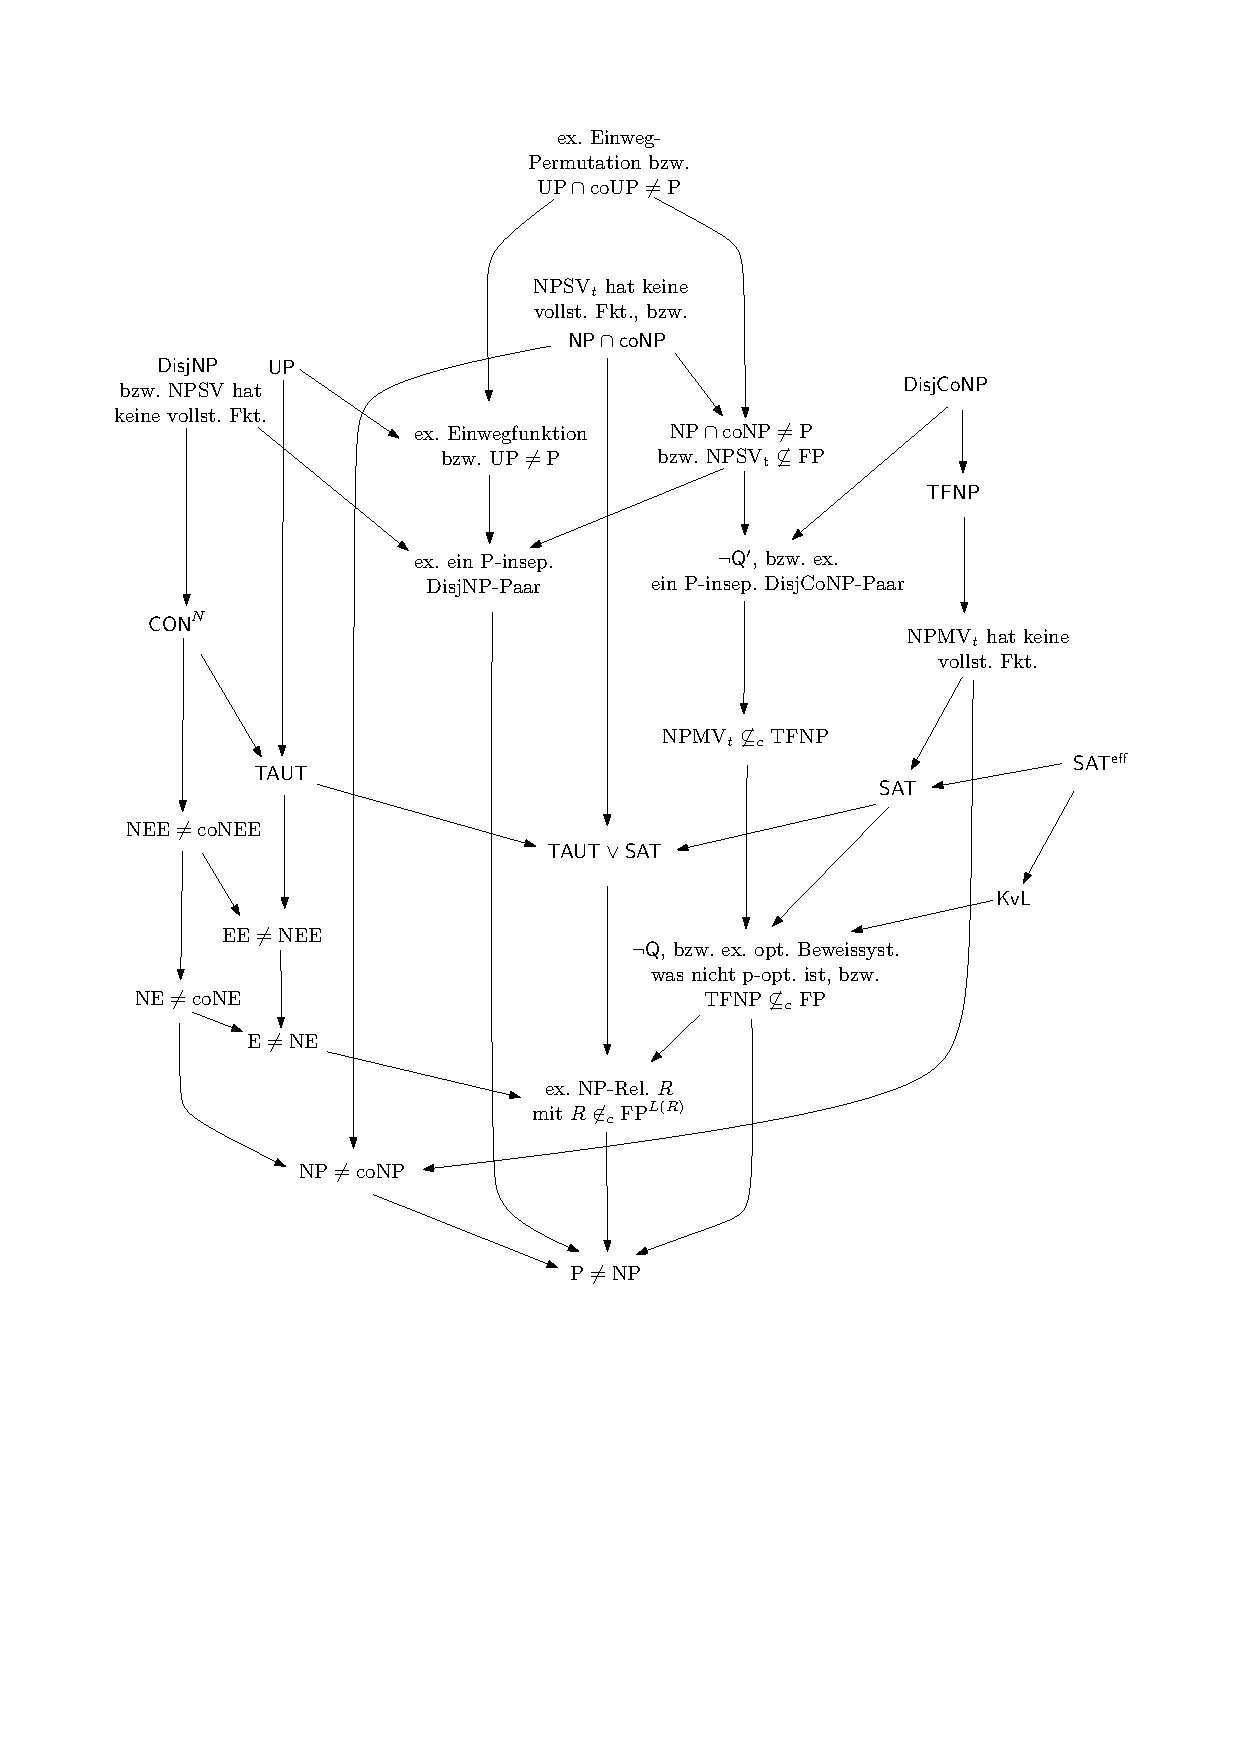
\includegraphics[page=1]{figures.pdf}
    \caption{Bekannte (relativierenden) Implikationen zwischen den betrachteten Hypothesen und weiteren Aussagen. Satz~\ref{thm:figure-implications} gibt Belegstellen für jede dieser Implikationen an.}\label{fig:figure-implications}
\end{figure}

Für alle dieser drei Desiderata ist es zunächst notwendig, auf die Hypothese $\hQ$ einzugehen.
\textcite{fenner_inverting_2003} beobachten, dass das Invertieren von surjektiven ehrlichen FP-Funktionen eine erstaunlich robuste Aussage ist, die eine Vielzahl von äquivalenten „fundamentalen“ \parencite{fenner_inverting_2003} Charakterisierungen aus der Komplexitätstheorie zulässt, so zum Beispiel die effiziente Lösbarkeit von TFNP-Suchproblemen, oder das effiziente Ausrechnen akzeptierender Rechenwege einer totalen NPTM. Wir können jetzt schon festhalten, dass die aktuelle Forschung diese Hypothese als sehr stark einschätzt, und eher die negative Beantwortung (i.e. $\neg\hQ$) vermutet.


\begin{theorem}[Äquivalente Formulierungen der Hypothese $\hQ$; \cite{fenner_inverting_2003}]\label{thm:q-orig}
    Folgende Aussagen sind äquivalent:
    \begin{enumerate}
        \item Hypothese $\hQ$.
        \item $\mathrm{NPMV}_t\subseteqc \mathrm{FP}$.
        \item $\TFNP\subseteqc \mathrm{FP}$.
        \item $\P=\NP\cap\coNP$ und $\mathrm{NPMV}_t\subseteqc \mathrm{NPSV}_t$.
        \item Jede surjektive ehrlichen Funktion $f\in\FP$ ist p-invertierbar.
        \item Für jede Menge $L\in \P$  und jede NPTM $N$ mit $L(N)=L$ existiert eine Funktion $h\in \FP$ mit 
            \[ x\in L \implies N(x) \text{ akz. mit Rechenweg $h(x)$}. \]
    \end{enumerate}
\end{theorem}

\textcite{fenner_inverting_2003} und \textcite{messner_simulation_2001} charakterisieren $\hQ$ noch durch zwei weitere Formen, diesmal über je eine Aussage über die Menge $\mathtt{SAT}$:

\begin{restatable}{theorem}{qfennermessner}\label{thm:q-fenner-messner}
    Folgende Aussagen sind äquivalent:
\begin{enumerate}[midpenalty=0,endpenalty=10000]
        \item Hypothese $\hQ$.
        \item \parencite{fenner_inverting_2003} Für jede NPTM $N$ mit $L(N)=\mathtt{SAT}$ existiert eine Funktion $h\in \FP$ sodass 
\[ N(\phi) \text{ akz. mit Rechenweg $w$} \implies \text{$h(w)$ ist eine erfüllende Belegung für $\phi$.} \]\pagebreak[2]
             
        \item \parencite{messner_simulation_2001} Das Standardbeweissystem $\mathit{sat}$
            \[ \mathit{sat}(\phi, w) = \begin{cases} \phi & \text{wenn $w$ eine erfüllende Belegung für $\phi$ ist} \\ \bot & \text{sonst.} \end{cases}\]
            für $\mathtt{rSAT}$ ist p-optimal.
    \end{enumerate}
    Dieser Satz relativiert nicht.
\end{restatable}

In anderen Worten sagt Aussage (2) aus, dass es modulo Umcodieren nur einen einzigen SAT-Solver gibt, und insbesondere alle SAT-Solver äquivalent zum trivialen Solver ist, welcher nur alle möglichen Belegungen ausprobiert.
Die Aussage (3) macht eine analoge Aussage über Beweissysteme: egal wie komplex ein Beweissystem $h$ für $\mathtt{SAT}$ ist, wir können immer einen $h$-Beweis für $\phi$ in eine erfüllende Belegung für $\phi$ (quasi ein trivialer Beweis für $\phi\in\mathtt{SAT}$) transformieren. Damit ist auch leicht zu sehen, dass $\hQ\Rightarrow \neg\hSAT$, zumindest im unrelativierten Fall.

In Abschnitt~\ref{sec:q-vs-search} werden wir sehen, dass sich die obigen Charakterisierungen auf weitere (aber möglicherweise nicht alle) vollständigen NP-Relationen generalisiert, womit insbesondere auch die beiden Charakterisierungen von \citeauthor{fenner_inverting_2003} und \citeauthor{messner_simulation_2001} zu einer \emph{relativierbaren} Variante verallgemeinert werden.
Mit dieser Verallgemeinerung ist es dann auch für uns möglich, $\hQ$ formal in das Pudláksche Programm (u.a. durch $\hQ\Rightarrow \neg\hSAT$) einzuordnen. Hierfür führen wir jetzt schon den Begriff eines Standardbeweissystems formal ein.

\begin{definition}[Standardbeweissystem einer NP-Relation]
    Sei $R$ eine NP-Relation. Wir definieren bezüglich $R$ das \emph{Standardbeweissystem} $\mathit{std}_R$ für $\Proj(R)$ wie folgt:
    \[ \mathit{std}_R(w) \defeq \begin{cases} x & \text{wenn $w=(x,y)$ und $(x,y)\in R$,}\\
    \bot & \text{sonst}.\end{cases} \qedhere \] 
\end{definition}
Damit ist, wie durch die Formulierung oben suggeriert, $\mathit{sat}=\mathit{std}_{\mathtt{rSAT}}$.
Bevor wir nun mit einer Diskussion zwischen Karp-Vollständigkeit und Levin-Vollständigkeit fortsetzen, schließen wir diesen Einstieg mit folgender einfachen Beobachtung ab:
\begin{observation}\label{obs:spps-honest}
    Für jede NP-Relation $R$ ist das Standardbeweissystem $\mathit{std}_R$ für $\Proj(R)$ ehrlich, optimal, und hat kurze Beweise.
\end{observation}
\begin{proof}
    Aus der p-Balanciertheit folgt sofort dass $\mathit{std}_R$ kurze Beweise hat. 
    Nach Beobachtung \ref{obs:super-ps-sind-opt} damit auch optimal.
    Insbesondere hat $\mathit{std}_R$ \emph{nur} polynomiell längere Beweise, also ist $\mathit{std}_R$ ehrlich.
\end{proof}
%\begin{proof}
    %Sei $q$ die Zertifikatsschranke von $R$, und sei $w=(x,y)$ gegeben sodass $\mathit{std}_R(x,y) = x$.
    %An dieser Stelle müssen wir auf die konkrete Codierung von Beweisen $w=(x,y)$ eingehen.
    %Wie in \ref{sec:notation} beschrieben, codieren wir Tupel in einer solchen Weise sodass
    %\[ |w| = |(x,y)| = 2(|x|+|y|+2) = 2|x|+ 2|y| + 4. \]
    %Da $(x,y)\in R$ gilt für $y$ auch $|y|\leq q(|x|)$.
    %Damit also
    %\[ |w| \leq 2|x|+ 2q(|x|) + 4 \leq q'(|x|) = q'(|\mathit{std}_R(w)|). \]
    %für ein geeignetes Polynom $q'$, wie gewünscht.
%\end{proof}

\section{Karp-Vollständigkeit vs. Levin-Vollständigkeit}\label{sec:karp-vs-levin}

Wir wiederholen hier erneut die zentrale offene Frage und Vermutung aus Abschnitt~\ref{sec:levin}:

\questionkvl*

\conjkvl*

Ich möchte argumentieren, dass die obige Frage bzw. Vermutung eng mit der Hypothese $\hQ$ zusammenhängt.
Im Speziellen werden wir sehen, dass die Hypothese $\hQ$ so charakterisiert werden kann, dass sie einer Verstärkung der Vermutung $\mathsf{KvL}$ entspricht.\sidenote{\textcite{fenner_inverting_2003} gaben hierbei eine ähnliche Aussage an (Cor.~3: „$\hQ$ holds iff every Karp reduction from $A$ to $B$ can be extended to a Levin reduction“), es ist aber hervorzuheben, dass die Autoren von einem unüblichen Begriff von Levin-Reduktionen ausgehen, der sich von dem hier verwendeten unterscheidet. Dieser umfasst nicht eine „Rückwärts-Translation“ von Zertifikaten für $B$-Instanzen zu $A$-Instanzen, sondern eine „Vorwärts-Translation“ von Zertifikaten für $A$-Instanzen zu $B$-Instanzen.}

\begin{theorem}\label{thm:q-as-levin}
    Folgende Aussagen sind äquivalent:
    \begin{enumerate}
        \item Hypothese $\hQ$, bzw. $\TFNP\subseteqc\FP$. 
        \item Für jedes Paar von NP-Relationen $A, B$ gilt:
            \[ \Proj(A) \leqmp \Proj(B) \iff A \leqlp B. \]
    \end{enumerate}
\end{theorem}
\begin{proof}
    \begin{prooflist}[label={}]
\item (1)$\implies$(2): Die Richtung von rechts nach links ist klar. Für die andere Richtung sei $\Proj(A) \leqmp \Proj(B)$ mit $A,B$ NP-Relationen. Sei $q$ hierbei das Polynom was die Zertifikatslänge in $A$ begrenzt.
    Wir wollen nun eine Levin-Reduktion von $A$ auf $B$ angeben. Sei $f\in \FP$ die Funktion, welche die Reduktion $\Proj(A) \leqmp \Proj(B)$ realisiert.

    Definiere folgende Relation $R$ mit
    \[ \fset{}R(w) = \begin{cases} \{ y\mid y\in\Sigma^{\leq q(|x|)}, (x,y)\in A \} & \text{falls $w=(x,y')$, $(f(x), y')\in B$} \\  \{\epsilon\} & \text{sonst}. \end{cases} \]
    Es ist leicht zu sehen, dass $R$ eine totale NP-Relation ist. Nach (1) existiert nun eine (totale) Verfeinerung $g\in \FP$ von $R$.

    Damit lässt die Levin-Reduktion von $A$ auf $B$ angeben: wähle $f$ als Reduktionsfunktion, und sei die Funktion $g$ von oben die Translationsfunktion. Dann gilt
    \begin{gather*}
        (f(x), y') \in B \implies (x, y')\in\Proj(R) \\
        \implies ((x, y'), g(x, y'))\in R\\
        \implies (x, g(x, y')) \in A \text{ nach Def. von $R$}
    \end{gather*}
    wie gewünscht. Wir haben $A\leqlp$ via $f, g$.
\item (2)$\implies$(1): Sei $A$ eine totale NP-Relation
    Definere nun die NP-Relation
    \[ B \defeq \{ (x, \epsilon) \mid x\in\Sigma^* \}. \]
    Es ist leicht zu sehen das $\Proj(A)=\Sigma^*=\Proj(B)$ und dass $\Proj(A)\leqmp\Proj(B)$ über die Identitätsfunktion.
    Nach Annahme (2) lässt sich nun diese Reduktion zu einer Levin-Reduktion $A\leqlp B$ verstärken, mit Reduktionsfunktion $f\in\FP$ und  Translationsfunktion $g\in\FP$.
    Für alle $x$ gilt nun $(f(x),\epsilon)\in B$ nach Definition,
    nach Levin-Reduktion also auch $(x, g(x, \epsilon))\in A$.
    Definieren wir nun $h(x)\defeq g(x,\epsilon)$, dann ist $(x, h(x))\in A$ für alle $x$, also $h\in\FP$ eine Verfeinerung von $A$, also $A\inc \FP$, wie gewünscht.
\end{prooflist}
\end{proof}

Beachte, dass in Aussage (2) die Implikation von rechts nach links ohnehin immer gilt. 
Damit lässt sich Aussage (2) auch so formulieren, dass jede Karp-Reduktion zu einer Levin-Reduktion verstärkt werden kann, indem zur Reduktionsfunktion $f$ eine geeignete Translationsfunktion $g$ hinzugefügt wird.
Mit dieser Charakterisierung folgt auch unmittelbar, dass $\hQ$ hinreichend für $\neg\mathsf{KvL}$ ist.


\begin{theorem}\label{thm:kvl-implies-q}
    $\mathsf{KvL} \implies \neg\hQ$.
\end{theorem}
\begin{proof}
    Wir zeigen die Kontraposition, und starten mit der Voraussetzung $\hQ$.
    Wir wollen nun $\neg\mathsf{KvL}$ zeigen. Sei hierfür $R$ eine beliebige NP-Relation sodass $\Proj(R)$ $\leqmp$-vollständig ist.
    Damit gilt also schon für alle weiteren NP-Relationen $A$, dass $\Proj(A)\leqmp\Proj(R)$.
    Nach Satz~\ref{thm:q} gilt also auch die Aussage \ref{thm:q}(6), und damit $A\leqlp R$. Also ist $R$ auch $\leqlp$-vollständig, wie gewünscht und wir haben $\neg\mathsf{KvL}$ gezeigt.
\end{proof}

Was sind natürlich notwendige Bedingungen für die Hypothese $\mathsf{KvL}$? Diese Frage erscheint tatsächlich wesentlich schwieriger als gedacht. Insbesondere scheint es unklar, ob aus irgend einer von Pudláks Hypothesen die Aussage $\mathsf{KvL}$ folgt.

Besonders interessant erscheint aber die Beziehung zur Hypothese $\neg\hQ$, also genau die Umkehrung von Satz~\ref{thm:kvl-implies-q}.
Zumindest in der obigen Charakterisierung von Satz \label{thm:q-as-levin} scheint $\neg\hQ$ schwächer, denn mit Satz \label{thm:q-as-levin} würde das bedeuten, dass ein \emph{beliebiges} Paar $A,B$ von NP-Relationen existiert mit $\Proj(A)\leqmp \Proj(B)$, aber $A \not\leq_\mathrm L^\mathrm p B$. Weder $A$ noch $B$ müssen eine $\leqmp$-vollständige Projektion haben, was $\mathsf{KvL}$ ja verlangt.

%, ist ja die Aussage (2) vom Satz~\ref{thm:q-as-levin} \emph{fast} in der Form „Karp-Vollständigkeit = Levin-Vollständigkeit“ ist.
Paradoxerweise scheint die Charakterisierung von $\neg\hQ$ durch \citeauthor{fenner_inverting_2003} in Satz~\ref{thm:q-fenner-messner}(2) dienlicher:
Betrachten wir hierbei exemplarisch den Fall Relationen für $\mathtt{SAT}$. Ich vermute, dass $\neg\hQ\Rightarrow \mathsf{KvL}$; um das zu plausibilisieren möchte ich zeigen, dass $\neg\hQ\land\neg\mathsf{KvL}$ unwahrscheinlich ist.

Starten wir mit $\neg\hQ$, dann gilt mit Satz~\ref{thm:q-fenner-messner} für alle Funktionen $h\in\FP$
\begin{equation} N(\psi) \text{ akz. mit Rechenweg $w$} \rlap{\hspace*{2pt}\raisebox{2.3pt}{$\quad\not$}}\implies  (\psi, h(\psi, w))\in\mathtt{rSAT}.\label{eq:weak-irreducibility} \end{equation}
In anderen Worten: es existiert zwar eine NPTM $N$ welche $\mathtt{SAT}$ entscheidet, aber aus den akzeptierenden Rechenwegen $w$ von $N(x)$ auf $x\in \mathtt{SAT}$ kann nicht effizient eine akzeptierende Belegung für $x$ abgeleitet werden.

Wir können $N$ äquivalent als NP-Relation $R_N$ repräsentieren, mit $(\phi, w) \in R_N$ genau dann wenn $N(x)$ mit Rechenweg $w$ akzeptiert.
Damit kann Gleichung~\ref{eq:weak-irreducibility} so verstanden werden, dass $\mathtt{rSAT} \not\leqlp R_N$ \emph{falls die Reduktionsfunktion $f$ die Identitätsfunktion ist}.

Unter der Annahme $\neg\mathsf{KvL}$ existiert nun eine Levin-Reduktion $\mathtt{rSAT}\leqlp R_N$ mit Reduktions- bzw. Translationsfunktion $f,g$. Das ist zunächst kein Widerspruch, denn es könnte ja $f\neq\mathrm{id}$.
%
%An dieser Stelle muss erneut hervorgehoben werden, dass im Allgemeinen $\mathtt{rSAT} \leqlp R_N$ mit Funktionen $f,g$ gelten kann, notwendig hierfür ist aber dass $f\neq\mathrm{id}$.
%
Gleichzeitig wäre die Existenz einer solchen Reduktion überraschend. Wir hätten nach Definition
\begin{equation}\label{eq:effective-simulation} N(f(\phi)) \text{ akz. mit Rechenweg $w$} \implies \phi \text{ wird von Belegung $g(\phi, w)$ erfüllt}. \end{equation}
Einerseits ist es also nicht möglich, aus dem Rechenweg $w$ effizient eine akzeptierende Belegung für $f(\phi)$ zu bestimmen, obwohl $w$ bezeugt dass $f(\phi)$ erfüllbar ist. (Ersetze in (\ref{eq:weak-irreducibility}) $\psi$ mit $f(\phi)$.)
Andererseits reicht der „Beweis“ $w$ aber aus, um (zusammen mit der Information $\phi$) effizient wieder eine erfüllende Belegung für $\phi$ zu berechnen. 
Das \emph{plausibilisiert} zwar einen Widerspruch, bzw. dass $\neg\hQ\land\neg\mathsf{KvL}$ wahrscheinlich falsch ist, ist aber natürlich kein solcher. Die Umkehrung von Satz~\ref{thm:kvl-implies-q} bleibt offen.

Dennoch vermute ich, dass solche Funktionen $f,g$ nicht jeweils für alle NPTM $N$ mit $L(N)=\mathtt{SAT}$ existieren können.
Tatsächlich können wir die eben formulierte Vermutung auch in der Theorie der Beweissystemen formulieren: hierfür können wir die beiden Aussagen aus Gleichung~\ref{eq:effective-simulation} je als Aussagen über „Beweissysteme“ verstehen. Links ist der Rechenweg $w$ der „Beweis“ für $f(\phi)\in \mathtt{SAT}$ über den Verifikator $N$, und rechts ist $g(\phi, w)$ die erfüllende Belegung für $\phi$, also ein $\mathit{sat}$-Beweis für $\phi\in\mathtt{SAT}$.

Um diese Idee nun zu formalisieren, definieren wir zunächst eine abgeschwächte Variante der p-Simulation.
\begin{definition}
    Seien $h,h'$ Beweissysteme für $L$. Das Beweissystem $h$ \emph{p-simuliert effektiv} $h'$ falls Funktionen $f,g\in\FP$ existieren sodass
    \begin{enumerate}
        \item $x\in L \iff f(x)\in L$,
        \item $ h'(w)=f(x) \implies h(g(x, w)) = x. $
    \end{enumerate}
    Wir schreiben in diesem Fall auch $h'\leq^\mathrm p_\mathrm{eff} h$. %\marginnote{\note{Nicht vergessen: es ist offenbar unklar, wie das Symbol $\leq$ bzgl. Simulation gebraucht wird. Dose/Glaßer würden in der Def. das Ordnungszeichen spiegeln, Krajíček/Pudlák dagegen genau so wie hier, Krajíček im Sammelband dagegen wieder gespiegelt.}}
\end{definition}
In anderen Worten, falls $h'\leq^p_\mathrm{eff} h$, dann kann $h$ zwar nicht \emph{jeden} $h'$-Beweis $w$ für $x\in L$ in einen $h$-Beweis für (das gleiche) $x$ effizient umrechnen, es kann aber zumindest alle \emph{relevanten} $h'$-Beweise effizient umrechnen, nämlich für jedes $x\in L$ die $h'$-Beweise für $f(x)$ in $h$-Beweise für $x$.
Anstelle „$h$ p-simuliert effektv $h'$“ ließe sich äquivalent auch $h^{-1}\leqlp h'^{-1}$ schreiben. Beachte, dass die Relation $h^{-1}$ nur Lösungen mit ihren Beweisen reliert.
Klar ist: p-Simulation impliziert effektive p-Simulation impliziert Simulation unter Beweissystemen.

Die obige Intuition lässt sich also folgendermaßen formulieren: ich vermute, zumindest unter der Annahme $\neq\hQ$, dass das Standardbeweissystem $\mathit{sat}$ nicht jedes Beweissystem effektiv p-simulieren kann, insbesondere nicht jenes was von $N$ induziert wird.
Wir können diese Vermutung auch allgemeiner ohne Bezugnahme auf $\mathtt{SAT}$ bzw. $\mathit{sat}$ formulieren:

\begin{conjecture}[$\mathsf{KvL}$ formuliert unter Beweissystemen]\label{conj:kvl-ps}
    Es existiert eine NP-Relation $Q$ mit $\leqmp$-vollständigem $\Proj(Q)$, wobei $\mathit{std}_Q$ nicht alle anderen optimalen Beweissysteme für $\Proj(Q)$ effektiv p-simulieren kann.

    %In anderen Worten, es existiert ein optimales Beweissystem $h$ für $\Proj(R)$ sodass $h\not\leq^\mathrm p_\mathrm{eff}  \mathit{std}_R$.
    %Das Standardbeweissystem $\mathit{sat}$ für $\mathtt{SAT}$ kann nicht alle anderen optimalen Beweissysteme für $\mathtt{SAT}$ effektiv p-simulieren.

    %In anderen Worten, es existiert optimales Beweissystem $h$ sodass $h\not\leq^\mathrm p_\mathrm{eff} \mathit{std}$.
\end{conjecture}
%Beachte, dass in der obigen Formulierung $\mathit{std}_R$ \emph{nicht} „effektiv p-optimal“ ist in dem Sinn, dass \emph{jedes} Beweissystem effektiv p-simuliert werden kann, sondern eben nur die optimalen Beweissysteme bzw. genau jene mit kurzen Beweisen.
Dass die Formulierung der Vermutungen \ref{conj:kvl} und \ref{conj:kvl-ps} äquivalent sind, zeigt folgende Beobachtung:
\begin{observation}\label{obs:kvl-equiv}
    %Sei $R$ eine NP-Relation mit $\leqmp$-optimalem $\Proj(R)$.
    %Sei $L$ eine $\leqmp$-vollständige Menge für $\NP$.
    Folgende Aussagen sind äquivalent:
    \begin{enumerate}
        \item Für jede NP-Relation $R$ mit $\leqmp$-vollständigem $\Proj(R)$ ist $R$ $\leqlp$-vollständig. (Das ist die Aussage $\neg\mathsf{KvL}$.)
        \item Für jede NP-Relation $Q$ mit $\leqmp$-vollständigem $\Proj(Q)$ kann $\mathit{std}_Q$ jedes optimale Beweissystem $h$ für $\Proj(Q)$ effektiv p-simulieren. (Das ist die Negation von der Vermutung~\ref{conj:kvl-ps}.)
        %\item Ist $\Proj(R)=L$, dann ist auch $R$ $\leqlp$-vollständig.
        %\item Ist $\Proj(R)=L$, dann gilt für alle optimalen Beweissysteme $h$ für $L$ auch $h\leq^\mathrm p_\mathrm{eff} \mathit{std}_R$.
    \end{enumerate}
\end{observation}
\begin{proof}
    \begin{prooflist}[label={}]
    \item (1)$\Rightarrow$(2): 
        Sei $R$ eine NP-Relation mit $\leqmp$-vollständigem $\Proj(R)$.
    Wir zeigen, dass $\mathit{std}_{R}$ jedes andere optimale Beweissystem $h$ effektiv p-simulieren kann.
    Nachdem $h$ optimal ist, hat es auch kurze Beweise (Beob.~\ref{obs:ps-for-np-optimal}): für jedes $x\in\Proj(R)$ existiert ein $h$-Beweis $w$ mit $|w|\leq q(|x|)$ für geeignetes Polynom $q$.  Definiere
    \[ R_h \defeq \{ (x, w) \mid |w|\leq q(|x|), h(w) = x\}. \]
    Diese Relation ist offenbar eine NP-Relation und $\Proj(R_h) = \Proj(R)$ und damit ist $\Proj(R_h)$ auch $\leqmp$-vollständig. 

    Nach Voraussetzung (1) ist also  $R_h$ auch $\leqlp$-vollständig.
    Insbesondere gilt also  auch $R \leqlp R_h$. Damit existieren also Funktionen $f,g\in\FP$ sodass
    $x\in \Proj(R) \leftrightarrow f(x)\in\Proj(R)$ und
    \[ (f(x), w) \in R_h \implies (x, g(x, w))\in R. \]
    Nach Definition gilt also 
    \[ h(w)=f(x) \implies \mathit{std}_R(g(x, w)) = x, \]
    und damit ist $h\leq^\mathrm p_\mathrm{eff} \mathit{std}_R$.

\item (2)$\Rightarrow$(1): 
    Sei $R$ eine NP-Relation wobei $\Proj(R)$ $\leqmp$-vollständig ist. Wir zeigen nun, dass $R$ auch $\leqlp$-vollständig ist.
    Sei hierfür $Q$ eine beliebige NP-Relation; wir wollen $Q\leqlp R$ zeigen.

    Aus der $\leqmp$-Vollständigkeit folgt unmittelbar die Existenz einer Reduktionsfunktion $f$ mit 
    \[ x\in \Proj(Q) \iff f(x) \in \Proj(R). \]
    Definiere
    \[ h(w) \defeq \begin{cases} x & \text{falls $w=(x,y)$ und $(f(x),y)\in R$} \\ \bot & \text{sonst.} \end{cases} \]
    Wir zeigen, dass $h$ ein Beweissystem für $\Proj(Q)$ ist. Es ist offenbar dass $h\in\FP$. Die Funktion $h$ ist korrekt: wenn $h(x,y)=x$ dann ist $f(x)\in\Proj(R)$ und nach Eigenschaft von $f$ auch $x\in\Proj(Q)$.
    Die Funktion $h$ ist vollständig: Sei $x\in\Proj(Q)$. Dann ist schon $f(x)\in\Proj(R)$ und es gibt ein $y$ mit $(f(x),y)\in R$. Also ist $(x,y)$ ein $h$-Beweis für $x$.

    Außerdem ist klar, dass $h$ kurze Beweise hat, damit ist $h$ auch optimal (Beob.~\ref{obs:ps-for-np-optimal}). % ist.\todo{warum?}
    Damit gilt nach (2) nun, dass $h\leq^\mathrm p_\mathrm{eff} \mathit{std}_Q$. Also existieren Funktionen $f',g'\in\FP$ sodass
    \[ x\in \Proj(Q)\iff f'(x)\in\Proj(Q),\quad h(w)=f'(x) \implies \mathit{std}_Q(g'(x,w))=x. \]%\implies (x,g(x,w))\in Q. \]
    Das reicht aus, $Q\leqlp R$ zu zeigen: wähle $f''(x)\defeq f(f'(x))$ als Reduktionsfunktion, dann gilt
    \begin{gather*}
        (f''(x), y)\in R \implies (f(f'(x)), y)\in R \implies h(\underbrace{f'(x),y}_{w})=f'(x) \\
    \implies \mathit{std}_Q(g'(x,w))=x \implies (x,g'(x,w))\in Q. \end{gather*}
    Die Translationsfunktion $g''$, welche $(x,y)$ zu $g'(x,w)$ übersetzt, lässt sich leicht angeben.
\end{prooflist}
\end{proof}

Mit der Definition der effektiven p-Simulation und der eben bewiesenen äquivalenten Formulierung der Karp-vs-Levin-Vermutung lässt sich nun zumindest die Hypothese $\hSAT$ so verstärken, dass diese hinreichend für $\mathsf{KvL}$ ist.


\begin{conjecture}[$\mathsf{SAT^{eff}}$]
    Keine $\leqmp$-vollständige Menge $L\in\NP$ hat ein optimales Beweissystem $h$, welches alle anderen optimalen Beweissysteme für $L$ effektiv p-simulieren kann. 
    %Es existiert eine Menge $L\in\NP$, und kein optimales Beweissystem für $L$ kann kann alle anderen optimalen Beweissysteme für $L$ effektiv p-simulieren.
    %In anderen Worten, für jedes optimales Beweissystem $h$ für $L$ existiert ein  optimales Beweissysteme $h'$ für $L$ sodass $h'\not\leq^\mathrm p_\mathrm{eff} h$.
\end{conjecture}

\begin{theorem}\label{thm:sateff-generalizes-sat}
    \begin{enumerate}
        \item $\mathsf{SAT^{eff}}\implies \hSAT$
        \item $\mathsf{SAT^{eff}}\implies \mathsf{KvL}$
    \end{enumerate}
\end{theorem}
\begin{proof}
\begin{prooflist}
\item Zu (1): Klar aus Kontraposition. Wenn für eine $\leqmp$-vollständige Menge $L\in\NP$ ein p-optimales Beweissystem $h$ für $L$ existiert, dann kann dieses (optimale) $h$ auch alle anderen Beweissysteme p-simulieren, und damit insbesondere auch alle optimalen Beweissysteme $h'$ effektiv p-simulieren.

\item Zu (2): Wieder klar aus Kontraposition. Unter $\neg\mathsf{KvL}$ folgt mit der Formulierung aus Vermutung~\ref{conj:kvl-ps} dass für jede NP-Relation $Q$, $\Proj(Q)$ vollständig, das (optimale) Standardbeweissystem $\mathit{std}_Q$ alle optimalen Beweissysteme für $\Proj(Q)$ effektiv p-simulieren kann. Das gilt dann insbesondere auch für die $\leqlp$-vollständige NP-Relation $\mathtt{rKAN}$, also hat die $\leqmp$-vollständige Menge $\mathtt{KAN}$ \emph{ein} Beweissystem, welches alle optimalen Beweissysteme effektiv p-simulieren kann.
\end{prooflist}
\end{proof}

Wir haben also je eine notwendige ($\neg\hQ$) und eine hinreichende Hypothese ($\mathsf{SAT^{eff}}$) für $\mathsf{KvL}$. 
Nichtsdestotrotz bleiben noch viele Fragen offen, die wir hier aus Platzgründen nicht weiter verfolgen werden. 
Wir konnten zwar $\mathsf{KvL}$ als Aussage über Beweissysteme formulieren, aber sind auch andere Charakterisierungen (z.B. ähnlich wie bei $\hQ$) möglich?
Gibt es natürliche (z.B. kryptographische) Annahmen die hinreichend für $\mathsf{KvL}$ sind? Wie ist die Beziehung zu den anderen Pudlákschen Hypothesen? Wie verhält sich insbesondere $\hSAT$ zu $\mathsf{SAT^{eff}}$? 
%Kann in Beobachtung~\ref{obs:kvl-equiv}(2) so verstärkt werden, dass $\mathit{std}_Q$ jedes (nicht nur die optimalen) Beweissystem effektiv p-simulieren kann, also gewissermaßen $\mathit{std}_Q$ „effektiv p-optimal“ ist?

Insgesamt ist durch die vorherigen Überlegungen aber ein erster Schritt getan, die Beziehung zwischen Levin- und Many-one-Vollständigkeit über die Vermutung $\mathsf{KvL}$ im Kontext des Pudlákschen Programms einzuordnen.
Weitere Forschung in diese Richtung erscheint vielversprechend.

\section{Hypothese $\hQ$ und Suchprobleme}\label{sec:q-vs-search}

Wie im Einstieg des Kapitels angesprochen, geben \textcite{fenner_inverting_2003} bzw. \textcite{messner_simulation_2001} äquivalente Charakterisierungen der Hypothese $\hQ$ an, welche sich im Wesentlichen auf auf der $\leqlp$-Vollständigkeit von $\mathtt{rSAT}$ aufbauen (Satz~\ref{thm:q-fenner-messner}).
Wir wiederholen hier noch einmal die Aussage, aber mit einer etwas abstrakteren Notation.
Ganz ähnlich wie NP-Relationen ein Standardbeweissystem induzieren, können wir auch das Standardbeweissystem bezüglich einer NPTM definieren:
\begin{definition}[Standardbeweissystem von NPTM]
    Sei $N$ eine NTM. Wir definieren bezüglich $N$ das das \emph{Standardbeweissystem} $\mathit{std}_N$ für $L(N)$ wie folgt:
    \[ \mathit{std}_N(w) \defeq \begin{cases} x & \text{wenn $w=(x,\alpha)$ und $N(x)$ akzeptiert auf RW $\alpha$,}\\
    \bot & \text{sonst}.\end{cases} \qedhere \] 
\end{definition}
Ähnlich wie bei Standardbeweissysteme für NP-Relationen ist $\mathit{std}_N$ für jede nichtdeterministische \emph{Polynomialzeit}-TM $N$ ehrlich, optimal, und hat kurze Beweise.
\begin{reptheorem}{Satz}{thm:q-fenner-messner}
    Folgende Aussagen sind äquivalent:
    \begin{enumerate}
        \item Hypothese $\hQ$.
        \item Für jede NPTM $N$ mit $L(N)=\mathtt{SAT}$ gilt $\mathit{std}_N\leqmp \mathit{sat}$. Es existiert also eine Funktion $h\in \FP$ sodass 
            \[ N(\phi) \text{ akz. mit Rechenweg $w$} \implies \text{$h(w)$ ist erfüllende Belegung für $\phi$}. \]
        \item Das Standardbeweissystem $\mathit{sat}$ für $\mathtt{rSAT}$ ist p-optimal.
    \end{enumerate}
    Dieser Satz relativiert nicht.
\end{reptheorem}

%\begin{itemize}
    %\item Für jede NPTM $N$ mit $L(N)=\mathtt{SAT}$ existiert eine Funktion $h\in \FP$ sodass 
    %\[ N(\phi) \text{ akz. mit Rechenweg $w$} \implies \mathit{std}_{\mathtt{rSAT}}(\phi, h(w)), \]
    %i.e. $h(w)$ ist eine erfüllende Belegung für $\phi$.
    %\item Das Standardbeweissystem $\mathit{std}_{\mathtt{rSAT}}$ ist p-optimal.
%\end{itemize}
Diese beiden Charakterisierungen wollen wir im Folgenden verallgemeinern und auf beliebige $\leqlp$-vollständige NP-Relationen $R$ übertragen. 
Hieraus ergibt sich schon unmittelbar der technische Beitrag, dass dann diese Charakterisierungen auch in einer relativierten Umgebung angewendet werden können, um z.B. ein geeignetes Orakel zu konstruieren, was $\hQ$ von anderen Hypothesen trennt.

Zweitens ergibt sich aus der Verallgemeinerung das überraschende Ergebnis, dass $\leqlp$-Vollständigkeit allein nicht ausreicht. In den originalen Beweisen von \citeauthor{fenner_inverting_2003} und \citeauthor{messner_simulation_2001} wurden stillschweigend zusätzliche Eigenschaften von $\mathtt{rSAT}$ mitgedacht und ausgenutzt. Die folgende Generalisierung deckt diese Eigenschaften auf, und plausibilisiert dass diese womöglich nicht von allen $\leqlp$-vollständigen NP-Relationen geteilt werden.

Eine dieser stärkeren Eigenschaften von $\mathtt{rSAT}$, welche \citeauthor{fenner_inverting_2003} in ihren Beweisen gebrauchten, ist die $\leq_\mathrm{1,i}^\mathrm p$-Vollständigkeit von $\mathtt{rSAT}$. Wir schwächen im Folgenden diese Voraussetzunt ab, und verlangen nur, dass eine NP-Relation unter ehrlichen Reduktionen vollständig ist. Dies gilt insbesondere für $\mathtt{rSAT}$.
Für welche $\leqlp$-vollständigen NP-Relationen das noch zutrifft, werden wir unten betrachten.

Mit dieser ehrlichen Levin-Vollständigkeit lässt sich nun die Charakterisierung von \citeauthor[Thm.~2]{fenner_inverting_2003} generalisieren:
\begin{lemma}\label{lemma:q-generalized}
    Sei $R$ eine $\leqlp$-vollständige NP-Relation, mit der zusätzlichen Eigenschaft dass für die jeweilige entsprechende Problem-Reduktionsfunktion $f\colon Q\to R$ für $Q\leqlp R$ immer gilt, dass $f$ ehrlich ist.
Folgende Aussagen sind äquivalent:
\begin{enumerate}
    \item Aussage $\hQ$.
    \item Für alle NPTM $N$ mit $L(N)=\Proj(R)$ lassen sich akzeptierende Rechenwege von $N$ in Zertifikate umrechnen: es gilt $\mathit{std}_N\leqmp \mathit{std}_R$, bzw. existiert eine Funktion $h\in\mathrm{FP}$ sodass
        \[ N(x) \text{ akz. mit Rechenweg $\alpha$} \implies (x,h(x,\alpha))\in R. \]
\end{enumerate}
\end{lemma}
\begin{proof}
\begin{prooflist}[label={}]
\item (1)$\Rightarrow$(2): 
    Nachdem $\hQ$ gilt, gilt auch $\TFNP\subseteqc\FP$ nach Beobachtung~\ref{obs:tfnp-q}.
    Sei nun $R$ eine beliebige NP-Relation mit Zertifikatsschranke $q$, und
    sei $N$ eine beliebige NPTM mit $L(N)=\Proj(R)$. 
    Definiere nun folgende Relation $Q$ mittels:
    \[ \fset{}Q(x, \alpha) \defeq  \begin{cases} \{ y\mid y\in\Sigma^{\leq q(|x|)}, (x,y)\in R \} & \text{falls $N(x)$ auf RW $\alpha$ akzeptiert,} \\\{\epsilon\} & \text{sonst.} \end{cases}\]
    Es ist leicht zu sehen, dass $Q$ eine totale NP-Relation ist. Insbesondere im ersten Fall gilt $x\in L(N)=\Proj(R)$, also existiert auch mindestens ein $y\in\fset{}R(x)$.

    Nach Annahme gilt also $Q\inc\FP$, sei also $h\in\FP$ eine Verfeinerung von $Q$.
    Nun gilt
    \begin{gather*}
        \mathit{std}_N(x,\alpha)=x\\
        \implies N(x) \text{ akz. mit Rechenweg $\alpha$}\\
        \implies \fset{}Q(x,\alpha) = \fset{}R(x)\\
        \implies h(x,\alpha) \in \fset{}R(x) \implies (x, h(x,\alpha))\in R,\\
        \implies \mathit{std}_R(x, h(x,\alpha))=x.
    \end{gather*}
    wie gewünscht.

\item (2)$\Rightarrow$(1): 
    Sei $Q\in\TFNP$. 
    Sei ferner $R$ eine $\leqlp$-vollständige NP-Relation unter ehrlichen Problem-Reduktionsfunktionen (z.B $\mathtt{rKAN}$), und Zertifikatsschranke $p$.
    Da $R$ ja vollständig ist, gilt $Q\leqlp R$ via $f,g\in\FP$ und (nach Voraussetzung) ist $f$ ehrlich; es existiert ein Polynom $q$ sodass $q(|f(x)|)\geq |x|$.

    Definiere nun die folgende NPTM $N'(w)$:\\%\marginnote{\tiny\note{Wichtig: Ehrlichkeit ist hier notwendig, denn wir \emph{müssen} das Urbild raten, und können das nicht als zweite Eingabe mitführen, damit $L(N')=\Proj(R)$. Auch alternative Wege über Beweissysteme laufen darauf hinaus, Levin-Paddability vorauszusetzen, woraus ohenhin wieder Ehrlichkeit folgt.}}\\
    \begin{algorithm}[H]
        Rate nichtdeterministisch $x\in \Sigma^{\leq q(|w|)}$\;
        \lIf{$f(x)=w$}{akzeptiere}
        \tcc{Ab hier kann man $x$ wegwerfen}
        Rate nichtdeterministisch $y\in \Sigma^{\leq p(|w|)}$\;
        Akzeptiere genau dann wenn $(w,y)\in R$.
    \end{algorithm}
    Wir zeigen nun, dass $L(N')=\Proj(R)$. Wir müssen hierfür nur die Fälle betrachten, wenn $N'(w)$ in Z.~2 akzeptiert.
    In diesem Fall gilt $f(x)=w$, und wir haben
    \[ x\in\Sigma^* \implies x\in\Proj(Q) \implies f(x)\in\Proj(R) \implies w\in\Proj(R), \]
    wie gewünscht.

    Nach (2) gilt nun also, dass eine Funktion $h\in\FP$ existiert sodass
    \[ N'(w) \text{ akz. mit Rechenweg $\alpha$} \implies (w,h(w,\alpha))\in R. \]
    Beobachte wie für $N'(f(x))$ immer ein trivialer akzeptierender Rechenweg $\alpha_x$ existiert: nämlich jener, welcher in Z.~1 das Urbild $x$ rät. Beobachte dass die Umformung $x\mapsto \alpha_x$ in Polynomialzeit möglich ist.

    Um nun (1) zu zeigen müssen wir aus $x\in\Sigma^*$ effizient einen akzeptierenden Rechenweg für $N$ bestimmen.
    Wir haben
    \begin{gather*}
        N'(f(x)) \text{ akz. mit Rechenweg $\alpha_x$} \implies (f(x),h(f(x),\alpha_x))\in R\\
        \implies (x, \underbrace{g(h(f(x), \alpha_x))}_{r(x)}) \in Q \quad\text{nach Translationsfunktion $g$}.
    \end{gather*}
    Damit ist $r\in \FP$, $r(x) \defeq  g(h(f(x), \alpha_x))$, eine Verfeinerung von $Q$ und $Q\inc\FP$, wie gewünscht.
\end{prooflist}
\end{proof}

Wir wollen nun auch die zweite Charakterisierung von \citeauthor{messner_simulation_2001} generalisieren.
Im originalen Beweis wurde erneut eine sekundäre stärkere Eigenschaft von $\mathtt{rSAT}$ ausgenutzt, die einer schwachen Form von Paddability entspricht. Ähnlich wie bei der Berman--Hartmanis-Paddability wollen wir beliebige Instanzen $x$ zu längeren Instanzen $x'$ vergrößern. Zusätzlich verlangen wir, dass wir auch auf Zertifikaten $y$ für $x'$ wieder Zertifikate $y$ für $x$ zurückrechnen können. In anderen Worten: wir codieren „redundante Teile“ in $x$ hinein, um $x'$ zu erhalten. Für Zertifikate $y'$ für $x'$ können wir dann den Teil des Zertifikats wegwerfen, welcher sich ohnehin nur auf das redundanten Padding bezieht, und erhalten wieder ein Zertifikat für $x$. 

\begin{definition}[Levin-Paddability]\label{def:levin-paddable}
    Eine NP-Relation $R$ ist \emph{Levin-paddable} wenn 
    Funktionen $\mathit{pad}\in\FP$ und $\mathit{padsol}\in\FP$ existieren, sowie ein Polynom $r$ sodass
    \begin{enumerate}
        \item $x\in \Proj(R) \iff \mathit{pad}(x, 1^n) \in \Proj(R)$,
        \item $(\mathit{pad}(x, 1^n), y)\in R \implies (x, \mathit{padsol}(x, 1^n, y)) \in R$,
        \item $r(|\mathit{pad}(x, 1^n)|)\geq n$. (Funktion $\mathit{pad}$ ist ehrlich bzgl. der zweiten Komponente.)\qedhere
    \end{enumerate}
\end{definition}
Beachte dass wir im Gegensatz zur Berman--Hartmanis-Paddability keine Invertierbarkeit der Padding-Funktion verlangen.
Später werden wir sehen, welche NP-Relationen alle diese Eigenschaft der Levin-Paddability erfüllen. Festhalten können wir aber, dass $\mathtt{rSAT}$ Levin-paddable ist. Das ist einfach zu sehen: padde Formeln $\phi$ auf, indem z.B. Disjunktionen neue Variablen hinzugefügt werden, i.e. 
\[ \phi' = \mathit{pad}(\phi, 1^n) = \phi \lor x_k \lor x_{k+1} \lor \cdots \lor x_{k+n}, \]
wobei $k$ hinreichend groß sein soll, dass $x_k, x_{k+1}, \dots$ nicht als Variable in $\phi$ vorkommt.
%Unter jeder vernünftigen Codierung gilt $|\mathit{pad}(x, 1^n)|\geq n$.
Ist nun $w'$ eine erfüllende Belegung für $\phi'$, dann entferne alle Variablenbelegungen $x_{k}, x_{k+1}, \dots$ aus $w'$; es ergibt sich eine erfüllende Belegung $w$ für $\phi$.

Diese Eigenschaft lässt sich auch leicht für die kanonische NP-Relation $\mathtt{rKAN}$ überprüfen, und gilt insbesondere auch im relativierten Fall.
\begin{observation}\label{obs:rkan-paddable}
    Die kanonische Levin-vollständige NP-Relation $\mathtt{rKAN}$ ist Levin-paddable.
\end{observation}
\begin{proof}[Skizze.]
    Padde Instanzen $(N, x, 1^n)$ zu $(N', x, 1^n)$ auf, wobei die NTM $N'$ aus $N$ hervorgeht, indem Zustände hinzugefügt werden die über die Transitionsrelation von $N$ nicht erreichbar sind. Ein akzeptierender Rechenweg auf $N'(x)$ ist dann genau ein akzeptierender Rechenweg auf $N(x)$.
\end{proof}


Mit dieser Definition können wir nun einen Beweis von \textcite[Thm. 5.2]{messner_simulation_2001} generalisieren. Beachte dass hier nicht notwendigerweise von vollständigen NP-Relationen gesprochen wird, und das im Beweis (3)$\Rightarrow$(1) die Levin-Paddability notwendig zu sein scheint, damit $\mathit{std}_R$ auch nicht-ehrliche Beweissysteme p-simulieren kann.
\begin{lemma}\label{lemma:stdps-q}
    Sei $R$ eine NP-Relation die Levin-paddable ist. Folgende Aussagen sind äquivalent:
    \begin{enumerate}
        \item Das Standardbeweissystem $\mathit{std}_R$ bzgl. $R$ ist p-optimal.
        \item Für alle NTM $N$ (ohne Laufzeitbeschränkung) mit $L(N)=\Proj(R)$ gilt $\mathit{std}_N\leqmp\mathit{std}_R$.
        \item Für alle NPTM $N$  mit $L(N)=\Proj(R)$ gilt $\mathit{std}_N\leqmp\mathit{std}_R$.
    \end{enumerate}
\end{lemma}
\begin{proof}
\begin{prooflist}[label={}]
\item (1)$\Rightarrow$(2): Klar.

\item (2)$\Rightarrow$(3): Klar.

\item (3)$\Rightarrow$(1): Angenommen (3) gilt. 
    Seien $\mathit{pad}$, $\mathit{padsol}$ die entsprechenden Funktionen, welche die Levin-Paddability von $R$ realisieren. Das Polynom $r$ sei so gewählt dass $r(|\mathit{pad}(x, 1^n)|)\geq n$ (vgl.~\ref{def:levin-paddable}(3)).

    Wir wollen nun zeigen, dass $\mathit{std}_R$ auch p-optimal ist. Sei hierfür $f$ ein beliebiges Beweissystem für $\Proj(R)$. Wir zeigen nun, dass $f\leqmp \mathit{std}_R$. Seien $\mathit{pad}$, $\mathit{padsol}$ die entsprechenden Padding-Funktionen von $R$.
    Definiere nun
    \[ f'(w) = \begin{cases} \mathit{pad}(x, 1^{|w|}) & \text{falls $w=1z$ und $f(z) = x$,} \\
    x & \text{falls $w=0z$ und $\mathit{std}_R(z)=x$,} \\ \bot & \text{sonst.} \end{cases} \]
    Es ist leicht zu sehen, dass $f'$ ein Beweissystem für $\Proj(R)$ ist. Außerdem ist $f'$ ehrlich es ist ehrlich für Eingaben $0z$, denn das Standardbeweissystem $\mathit{std}_R$ ist ehrlich nach Beobachtung~\ref{obs:spps-honest}. Es ist ehrlich für Eingaben $w=1z$, denn
    \[ |1z| = |w| \leq r(|\underbrace{\mathit{pad}(x, 1^{|w|})}_{f'(1z)}|) = r(|f'(|w|)|). \]
    Sei im Folgenden dann das Polynom $r'$ so gewählt, dass $|w|\leq r'(|f'(w)|)$ gilt.

    Definiere nun die NPTM $N_{f'}$ welche auf Eingabe $x$ erst nichtdeterministisch einen Beweis $w$, $|w|\leq r'(|x|)$ rät, und genau dann akzeptiert falls $f'(w)=x$.
    Es ist klar, dass $L(N_{f'}) = \Proj(R)$.
    Nach Voraussetzung (3) gilt $\mathit{std}_{N_{f'}}\leqmp \mathit{std}_R$, es gibt es also nun eine Funktion $h\in\FP$ sodass 
    \begin{equation} N_{f'}(x) \text{ akz. mit Rechenweg $\alpha$} \implies (x,h(x,\alpha))\in R.  \label{eq:stdps-q-1}
    \end{equation}

    Jetzt können wir zeigen, dass $\mathit{std}_R$ das Beweissystem $f$ p-simuliert: sei $z$ ein $f$-Beweis für $x$, d.h. $f(z)=x$.
    Wir wissen, dass $f'(1z)=\mathit{pad}(x, 1^{|1z|})=x'$.
    Daher können wir aus $z$ einen Rechenweg $\alpha_z$ konstruieren, sodass $N_{f'}(x')$ akzeptiert, nämlich jener der den $f'$-Beweis $1z$ rät.
    Die Abbildung $z\mapsto \alpha_z$ lässt sich in Polynomialzeit leisten.

    Nun gilt
    \begin{gather*}
        N_{f'}(x') \text{ akz. mit $\alpha_z$ } \implies (x', \underbrace{h(x', \alpha_z)}_{y'})\in R \text{ nach (\ref{eq:stdps-q-1})}\\
        \implies (\mathit{pad}(x, 1^{|1z|}), y')\in R \text{ mit $y'=h(x', \alpha_z)$ und obiger Def. von $x'$} \\
    \implies (x, \underbrace{\mathit{padsol}(x, 1^{|1z|}, y')}_y) \in R \text{ nach Def. \ref{def:levin-paddable}(2)}\\
        \implies \mathit{std}_R(x, y)=x \text{ mit $y=\mathit{padsol}(x, 1^{|1z|}, y')$}
    \end{gather*}
    und wir haben aus dem $f$-Beweis $z$ für $x$ einen $\mathit{std}_R$-Beweis $(x,y)$ für $x$ bestimmt.
    Es ist klar, dass die Übersetzung $z\mapsto (x,y)$ in Polynomialzeit möglich ist.
\end{prooflist}
\end{proof}

Wir fassen kurz den aktuellen Stand zusammen. \marginnote{\todo{Irgendwie möglich von $\mathit{std}_N$ wegzukommen und stattdessen über z.B.  ps mit kurzen Beweisen zu sprechen?}} Sei $R$ eine NP-Relation. 
Wir haben nun folgendes Bild:

\begin{center}
\begin{tikzpicture}[node distance=2cm, every node/.style={inner xsep=10pt}]
    \node (A) {$\hQ$};
    \node (B) [right=of A, align=center] {$\mathit{std}_N \leqlp\mathit{std}_R$ für alle\\ NPTM $N$ die $\Proj(R)$ entsch.};
    \node (C) [right=of B] {$\mathit{std}_R$ ist p-opt.};

    \draw[implies-,double equal sign distance,bend left=30] ([yshift=5pt]A.east)  to node[above] {\it\small falls $R$ ehrlich Levin-vollst.} ([yshift=5pt]B.west);
    \draw[-implies,double equal sign distance,bend left=30] ([yshift=5pt]B.east)  to node[above] {\it\small falls $R$ Levin-paddable} ([yshift=5pt]C.west);

    \draw[-implies,double equal sign distance,bend right=30] ([yshift=-5pt]A.east)  to node[above] {} ([yshift=-5pt]B.west);
    \draw[implies-,double equal sign distance,bend right=30] ([yshift=-5pt]B.east)  to node[below] {} ([yshift=-5pt]C.west);

    \draw[draw=none] (A.east)  -- (B.west) node[midway] {(\ref{lemma:q-generalized}) };
    \draw[draw=none] (B.east)  -- (C.west) node[midway] {(\ref{lemma:stdps-q}) };
\end{tikzpicture}
\end{center}

Wir wollen nun eine möglichst breite Klasse an NP-Relationen angeben, für die diese beiden obigen Äquivalenzen gelten, also insbesondere diejenigen NP-Relationen, welche die selbe Charakterisierung wie $\mathtt{rSAT}$ im Fall der unvelativierbaren Charakterisierung von \citeauthor{fenner_inverting_2003} und \citeauthor{messner_simulation_2001} zulassen.

Wir überlegen uns hierzu zunächst, dass „$\leqlp$-vollständig und Levin-paddable“ ausreichend ist, da Levin-Paddability insbesondere zulässt, eine Levin-Reduktion so zu padden, dass die Reduktionsfunktion auch ehrlich ist.
\begin{lemma}
    Die in Lemma~\ref{lemma:q-generalized} und~\ref{lemma:stdps-q} genannten Voraussetzungen an die NP-Relation $R$ werden von allen solchen $R$ erfüllt, die $\leqlp$-vollständig sind und Levin-paddable sind.
\end{lemma}
\begin{proof}
    Es ist sofort klar, dass $R$ die Voraussetzungen von Lemma~\ref{lemma:stdps-q} erfüllt.
    Es bleibt nur zu zeigen, dass für jede NP-Relation $Q$ eine $\leqlp$-Reduktion angegeben werden kann, bei dem die Problem-Reduktionsfunktion ehrlich ist.
    Wir nutzen hierbei aus, dass $R$ eine Levin-paddable Relation ist.

    Nachdem $R$ vollständig ist, gilt $Q\leqlp R$; sei $f,g\in\FP$ die Reduktions- bzw. Translationsfunktion welche diese Reduktion realisieren. Wir werden nun Funktionen $f', g'\in\FP$ angeben, welche die gleiche Reduktion realisieren, aber $f'$ ehrlich, wie gewünscht.

    Sei $\mathit{pad}, \mathit{padsol}$ die zu $R$ zugehörigen Padding-Funktionen. Definiere
    \[ f'(x) \defeq  \mathit{pad}(f(x), 1^{|x|}). \]
    Es gilt
    \[ x\in\Proj(Q) \iff f(x)\in \Proj(R) \iff \mathit{pad}(f(x), 1^{|x|})=f'(x)\in\Proj(R), \]
    wobei erste Implikation die Eigenschaft der Reduktionsfunktion $f$ ist, und die zweite aus der Definition von Levin-Paddability folgt.
    Aus der Definition von  Levin-Paddability folgt auch $r(|f'(x)|)\geq |x|$ für ein geeignetes Polynom $r$, und damit ist auch $f'$ ehrlich.

    Definiere
    \[ g'(x, z) \defeq  g(x, \mathit{padsol}(f(x), 1^{|x|}, z)). \]
    Sei nun $(f'(x), z)\in R$. Die Funktion $g'$ berechnet nun ein Zertifikat $y$ für $x$: Wir haben $(\mathit{pad}(f(x), 1^{|x|}), z)\in R$, also gilt nach Levin-Paddability dass \[(f(x), \mathit{padsol}(f(x), 1^{|x|}, z))\in R,\] 
    und nach Definition der Translationsfunktion $g$ gilt dann
    \[(x, g(x, \mathit{padsol}((f(x), 1^{|x|}, z)))\in Q,\]
    und das ist genau $(x, g'(x, z))\in Q$, wie gewünscht.
\end{proof}

Folgende Beobachtung hilft uns, natürliche NP-Relationen zu identifizieren, welche Levin-vollständig und gleichzeitig Levin -paddable sind.
\begin{observation}\label{obs:invcomplete-sind-levinpaddable}
    %Jede $\leq_\mathrm{L,inv}^\mathrm{p}$-vollständige NP-Relation $R$ ist auch Levin-paddable.
    \begin{enumerate}
        \item Gilt $\mathtt{rKAN}\leq_\mathrm{L}^\mathrm{p} R$, und ist die zugehörige Reduktionsfunktion $f$ ehrlich, dann ist $R$ Levin-paddable (und $\leqlp$-vollständig).
        \item Jede $\leq_\mathrm{L,1,inv}^\mathrm{p}$-vollständige NP-Relation $R$ ist auch Levin-paddable.
    \end{enumerate}
\end{observation}
Damit können wir schon als Ergebnis festhalten, dass 
jede $\leq_\mathrm{L,1,inv}^\mathrm{p}$-vollständige Relation $R$ die in 
Lemma~\ref{lemma:stdps-q} und~\ref{lemma:q-generalized} genannten Voraussetzungen an die NP-Relation $R$ erfüllt.
Das sind nach \textcite{goldreich_computational_2008} unrelativierten Fall u.a. $\mathtt{rSAT}$, $\mathtt{rSETCOVER}$, $\mathtt{rVERTEXCOVER}$, $\mathtt{rCLIQUE}$, $\mathtt{r3COLORABILITY}$.

\medskip
\begin{proof}[Beweis zu Beobachtung~\ref{obs:invcomplete-sind-levinpaddable}]
    Aussage (2) folgt unmittelbar aus (1): Wir haben $\mathtt{rKAN}\leq_\mathrm{L,1,inv}^\mathrm{p} R$ und damit ist die entsprechende Reduktionsfunktion $f$ p-invertierbar, und damit ehrlich.

    Für (1) nutzen wir die Levin-Paddability von $\mathtt{rKAN}$ aus: übersetze Instanz $x$ von $R$ nach $\mathtt{rKAN}$, padde dort hoch, und übersetze zu $R$-Instanz $x'$ zurück. Ist dann $y'$ ein Zertifikat für $x'$, dann lässt sich dies auf ähnlichem Weg wieder zu einem Zertifikat für $x$ zurückrechnen.

    Seien $f, g$ die Reduktions- bzw. Translationsfunktion, welche $\mathtt{rKAN}\leq_\mathrm{L}^\mathrm p R$ bezeugen, und seinen analog $f', g'$ jene Funktionen, welche $R\leq_\mathrm{L}^\mathrm p \mathtt{rKAN}$ bezeugen. Erstere existieren nach Voraussetzung, zweitere existieren weil $\mathtt{rKAN}$ $\leq_\mathrm{L}^\mathrm p$-vollständig ist.
    Nach Voraussetzung ist $f$ ehrlich. %, und da $f'$ p-invertierbar ist, ist auch $f'$ ehrlich. 
    Und nach Beobachtung~\ref{obs:rkan-paddable} existieren für $\mathtt{rKAN}$ Padding-Funktionen $\mathit{pad}_\mathtt{rKAN}$, $\mathit{padsol}_\mathtt{rKAN}$.
    Sei $q$ ein entsprechendes Polynom mit $q(|\mathit{pad}_\mathtt{rKAN}(x, 1^n)|)\geq n$, $q(|f(x)|) \geq |x|$.

    Definiere nun
    \[ \mathit{pad}_R(x, 1^n) \defeq  f(\mathit{pad}_\mathtt{rKAN}(f'(x), 1^n)). \]
    Die Zugehörigkeit zu $\Proj(R)$ bleibt erhalten:
    \begin{gather*}
        x\in \Proj(R) \iff f'(x) \in \mathtt{KAN} \iff \mathit{pad}_\mathtt{rKAN}(f'(x), 1^n) \in \mathtt{KAN}\\ \iff f(\mathit{pad}_\mathtt{rKAN}(f'(x), 1^n)) \in \Proj(R) \iff \mathit{pad}_R(x, 1^n) \in\Proj(R).
    \end{gather*}
    Ferner gilt
    \begin{align*} &q(q(|\mathit{pad}_R(x, 1^n)|)) \\&= q(q(|f(\mathit{pad}_\mathtt{rKAN}(f'(x), 1^n)|))\\&\geq q(|\mathit{pad}_\mathtt{rKAN}(f'(x), 1^n)|)\\ &\geq n.
    \end{align*}
    und damit ist $\mathit{pad}_R$ wie gewünscht ehrlich bzgl. $n$ (mit Polynom $q\circ q$).

    Es verbleibt noch die Funktion $\mathit{padsol}_R$. Nehme hierfür an dass wir ein $y'$ haben mit $(\mathit{pad}_R(x, 1^n), y')\in R$.
    Wir können über $g, g'$ das Zertifikat $y'$ zu Zertifikat $y$ mit $(x, y)\in R$ zurück übersetzen:
    Sei $p\defeq \mathit{pad}_\mathtt{rKAN}(f'(x), 1^n)$, dann gilt
    \[ (f(p), y')\in R \implies (p, \underbrace{g(p, y')}_z)\in \mathtt{rKAN}. \]
    Definiere $z=g(p, y')$.
    Nun haben wir
    \begin{gather*} (p, z)=(\mathit{pad}_\mathtt{rKAN}(f'(x), 1^n), z)\in\mathtt{rKAN}  \\\quad\implies (f'(x), \underbrace{\mathit{padsol}_\mathtt{rKAN}(f'(x), 1^n, z)}_{z'})\in\mathtt{rKAN} \end{gather*}
    und mit $z'=\mathit{padsol}_\mathtt{rKAN}(f'(x), 1^n, z)$ gilt
    \[ (f'(x), z') \in \mathtt{rKAN} \implies (x, \underbrace{g'(x, z')}_{y}) \in R. \]
    %\[ \mathit{padsol}_R(x, 1^n, y') = g(\mathit{pad}_\mathtt{rKAN}(f'(x), 1^n), y')
    %\[ q(q(q(|\mathit{pad}_R(x, 1^n)|))) = q(q(q(|f(\mathit{pad}_\mathtt{rKAN}(f'(x), 1^n))|)))
    Es ist leicht zu sehen, dass sich eine Funktion $\mathit{padsol}_R\in\FP$ angeben kann, die aus $x, 1^n, y'$ dieses entsprechende $y$ berechnen kann.
\end{proof}

Anstelle der Betrachtung, wie die \emph{Reduktionen} zwischen den einzelnen NP-Relationen aufgebaut sind, können wir auch strukturelle Eigenschaften von NP-Relationen ausnutzen, um Paddability zu zeigen. Hierbei macht die Definition von \emph{Universalität} durch \textcite{agrawal_universal_1992} aus dem Abschnitt~\ref{sec:gemeinsame-struktur} einen produktiven Beitrag. Ist eine NP-Relation \emph{joinable}, dann können wir auch zu einer Instanz beliebig viele Dummy-Instanzen anhängen. Aufgrund der speziellen Eigenschaften der $\mathit{join}$-Funktion können wir auch den relevanten Teil aus Zertifikaten für die verlängerten Instanz zielgenau auslesen. 

\begin{observation}\label{obs:joinable-sind-levinpaddable}
    %Jede universelle Relation ist Levin-paddable. Dieses Resultat gilt nur im unrelativierten Fall.
    Jede strenge NP-Relation $R\neq\emptyset$ die \emph{joinable} ist, ist auch Levin-paddable. 
\end{observation}
Vor dem Beweis können wir mit dieser Aussage festhalten, dass jede universelle Relation $R$ die in 
Lemma~\ref{lemma:stdps-q} und~\ref{lemma:q-generalized} genannten Voraussetzungen an die NP-Relation $R$ erfüllt.
Das sind nach \textcite{agrawal_universal_1992} u.a. $\mathtt{rSAT}, \mathtt{rHAM}, \mathtt{rINDSET}, \mathtt{rKNAPSACK}, \mathtt{rMAXCUT}$.

\medskip
\begin{proof}[Beweis zu Beobachtung~\ref{obs:joinable-sind-levinpaddable}]
    Sei $R$ eine NP-Relation, mit zugehörigem Polynom $q$, welches die Zertifikatsgröße spezifiziert. Zur Erinnerung, nachdem $R$ streng ist, gilt $(x,y)\in R \Rightarrow |y|=q(|x|)>0$.
    Ferner haben wir eine Instanz $z\in\Proj(R)$. Damit existiert also auch ein $w$ mit $(z,w)\in R$ und $q(|z|)=|w|>0$.

    Wir zeigen zunächst, wie wir für beliebige Instanz $x$ und $n\in\mathbb N$ auf eine Instanz $x'$ hochpadden, in dem Sinne dass $q(|x'|) \geq n$.
    Nach Voraussetzungen  ist die Relation $R$ auch \emph{joinable}, das heißt wir haben eine Funktion $\mathit{join}\in\FP$. Sei 
    \[ (x',\delta)\defeq \mathit{join}(x, \underbrace{z, z, \ldots, z}_{\text{$n$ mal}}).\]
    %Wir werden nun über die Länge $|\delta|$ auf die Länge von Zertifikaten zu $x'$ schließen, und damit $|x'|$ beschränken.
    Intuitiv muss nun $\delta$ (und damit $x'$) lang sein, da nun aus all den $n$ vielen Instanzen $z$ wieder das jeweilige Zertifikat aus jedem Zertifikat für $x'$ extrahiert werden muss.
    Nach Definition~\ref{def:universal} gilt
    \[ q(|x'|) \geq |\delta|=q(|x|) + \underbrace{q(|z|) + \cdots + q(|z|)}_{\text{$n$ mal}} \geq  n\cdot q(|z|) \geq n. \]
    %Beob. dass unter Definition ?? alle Zertifikate $y'$ für $x'$ die feste Länge $q(|x'|)$ haben. 
    %Zur Erinnerung: wir haben
    %\begin{align}\label{eq:levinpad-join} &\{ y'[\delta] \mid y'\in\fset{}R(x') \} = \{ yy_1y_2\cdots y_{n} \mid y\in\Sigma^{q(|x|)}, y_1,y_2, \ldots \in \Sigma^*, y\in\fset{}R(x), y_1,y_2,\dots,y_n\in\fset{}R(z) \} \end{align}
    %Die Sequenz $\delta$ besteht nach Definition aus paarweise verschiedenen Indizes, daher können wir argumentieren, dass auch alle Zertifikate $y'$ (mit vorgegebener Länge $q(|x'|)$) mindestens die Länge $|\delta|$ haben.
    %Damit gilt
    %\[ q(|x'|) \geq |\delta| \geq n \]
    %wie gewünscht.

    Sei nun $\mathit{pad}$ genau jene polynomialzeit-berechenbare Funktion, die aus $x$ und $1^n$ die Instanz $x'$ konstruiert:
    \[ \mathit{pad}(x, 1^n) \defeq  x' \quad\text{ wobei }
    (x',\delta)=\mathit{join}(x, \underbrace{z,z,\ldots, z}_{\text{$n$ mal}}).\]
    Dann gilt schon sofort, dass $q(|\mathit{pad}(x, 1^n)|)=q(|x'|)\geq n$ wie gewünscht.

    Wir zeigen jetzt, dass die Zugehörigkeit zu $\Proj(R)$ erhalten bleibt.
    Zur Erinnerung, wir haben nach Eigenschaften der $\mathit{join}$-Funktion
    \begin{align}\label{eq:levinpad-join} &\{ y'[\delta] \mid y'\in\fset{}R(x') \} = \{ yy_1y_2\cdots y_{n} \mid  y\in\fset{}R(x), y_1,y_2,\dots,y_n\in\fset{}R(z) \}. \end{align}
    Gilt $x\not\in\Proj(R)$, dann ist die rechte Menge in (\ref{eq:levinpad-join}) leer, also auch die linke Menge und damit $x'=\mathit{pad}(x, 1^n)\not\in \Proj(R)$.
    Falls anders herum $x\in\Proj(R)$, dann ist die rechte Menge nicht leer, existiert ja ein Zertifikat $y$ für $x$ und je ein $y_i=w$ für jedes $z$. Also ist auch die linke Menge nicht leer, damit $\mathit{pad}(x, 1^n)\in \Proj(R)$.

    Die noch verbleibende Funktion $\mathit{padsol}$ ist durch die bitweise Projektion durch $\delta$ leicht möglich:
    \[
    \mathit{padsol}(x, 1^n, y') \defeq  y'[\delta][0, 1, \ldots, q(|x|)-1] \enspace\text{ wobei } (\cdot, \delta) = \mathit{join}(x, \underbrace{z,z,\ldots, z}_{\text{$n$ mal}}).\]
    Wir verifizieren: Sei $(\mathit{pad}(x, 1^n), y')\in R$, dann ist nach (\ref{eq:levinpad-join}) $y'[\delta]=yy_1y_2\cdots$ wobei $(x,y)\in R$. Nachdem $R$ streng ist, gilt insbesondere $y\in\Sigma^{q(|x|)}$ und wir haben
\[ \mathit{padsol}(x, 1^n, y') = y'[\delta][0, 1, \ldots, q(|x|)-1] = (yy_1y_2\cdots)[0,1,\ldots,q(|x|)-1] = y \]
    und damit $(x, \mathit{padsol}(x, 1^n, y')) = (x, y)\in R$, wie gewünscht.
\end{proof}

Es bleibt die Frage offen, ob Levin-Paddability für \emph{alle} vollständigen NP-Relationen zutrifft. Unter Annahmen einer geeigneten Einwegfunktion ist dies nicht der Fall.
Die Argumentation verläuft hier ähnlich zur \emph{Encrypted Complete Set Conjecture}.
Wir setzen hier eine stärkere \emph{secure one-way function} \parencite{grollmann_complexity_1988} $f$ voraus, die selbst mithilfe funktionaler Orakel-Queries nur auf einer dünnen Menge p-invertierbar ist.
Präzise meinen wir damit folgendes: sei $A$ ein beliebiger Polynomialzeit-Algorithms, der auf Eingabe $w$ versucht, das Urbild $f^{-1}(w)$ zu berechnen. Zusätzlich darf $A$ das Urbild $f^{-1}(w')$ von einem Wort $w'\neq w$ erfragen. Selbst dann wird $A$ nur auf einer dünnen Menge $W\subseteq\Sigma^*$ das korrekte Urbild aller $w\in W$ bestimmen können.
(Vgl. die Ähnlichkeit zur Selbstreduzierbarkeit aus Abschnitt~\ref{sec:search-vs-decision}.)
Die Existenz einer solchen Einwegfunktion erscheint aus kryptographischer Perspektive naheliegend.

Betrachte nun, analog zur Encrypted Complete Set Conjecture, die NP-Relation
\[ Q = \{ (f(\phi), (\phi, z)) \mid x,z\in\Sigma^*, (\phi,z)\in\mathtt{rSAT}\}. \]
Es ist leicht zu sehen dass $\mathtt{rSAT}\leqlp Q$ und damit ist $Q$ auch $\leqlp$-vollständig.
Gleichzeitig kann dann $Q$ nicht Levin-paddable sein.
Denn angenommen, $Q$ ist Levin-paddable, dann lässt sich $f$ mit einem funktionalen Orakel-Query \emph{zumindest auf den Werten $f(\mathtt{SAT})$} p-invertieren: gegeben $w\in f(\mathtt{SAT})$, berechne erst eine zweite Instanz $w'=\mathit{pad}(w, 1^n)\in\Proj(Q)$ mit hinreichend langem $n$ sodass $w'\neq w$. Frage dann an das Orakel und erhalte $(x',z')\in \fset{}Q(w')$.
Dann gilt $(x,z) = \mathit{padsol}(w, 1^n, (x',z'))$ mit $f(x)=w$, i.e. $x$ ist das gesuchte Urbild von $w$.
Wir können also auf der Bildmenge  $f(\mathtt{SAT})$ die Einwegfunktion $f$ invertieren.
Diese Menge ist tatsächlich nicht dünn: unabhängig der gewählten Codierung von $\mathtt{SAT}$ folgt aus der Existenz der Einwegfunktion $f$ schon $\P\neq\NP$, und damit ist insbesondere die $\leqmp$-vollständige Menge $f(\mathtt{SAT})$ eine nicht-dünne Menge nach dem Satz von \textcite{mahaney_sparse_1982}.
Das widerspräche nun den Eigenschaften von $f$, also ist $Q$ nicht Levin-paddable.
(Diese Argumentation relativiert, wenn anstelle $\mathtt{rSAT}$ eine relativierbare vollständige Menge gewählt wird, die z.B $\mathtt{rKAN}$.)

Dennoch bleibt die allgemeine Frage zwischen $\leqlp$-Vollständigkeit und Levin-Paddability offen, die wir im Folgenden nicht weiter bearbeiten werden:
\begin{question}
    Ist jede $\leqlp$-vollständige NP-Relation $R$ auch Levin-paddable?
    Existiert ggf. ein Gegenbeispiel in einer geeigneten relativierten Umgebung?
\end{question}

%\section{Hypothese $\hQ$ und das Pudláksche Programm}

Unabhängig von dieser Frage können wir nun aber abschließend die vorigen Ergebnisse zur Beziehung zwischen Suchproblemen und der Hypothese $\hQ$ in folgendem Satz zusammenfassen.
Beachte dass diese Charakterisierungen relativieren.
Die Äquivalenz zu Aussage (8) ist hierbei eine einfache relativierbare Generalisierung von Beweisen durch \textcite[Thm.~5.3]{messner_simulation_2001}.

\begin{theorem}[Äquivalente Formulierungen der Hypothese $\hQ$]\label{thm:q}
    Folgende Aussagen sind äquivalent:
    \begin{enumerate}
        \item Hypothese $\hQ$: Für jede NPTM $N$ mit $L(N)=\Sigma^*$ existiert eine Funktion $g\in\FP$ sodass für alle $x$ das Bild $g(x)$ ein akzeptierender Rechenweg von $N(x)$ ist.
        \item $\TFNP\subseteqc \FP$
        \item $\mathrm{NPMV}_t\subseteqc \FP$
        \item $\P=\NP\cap\coNP$ und $\mathrm{NPMV}_t\subseteqc \mathrm{NPSV}_t$
        \item Jede surjektive ehrliche Funktion $f\in\FP$ ist p-invertierbar, heißt die Umkehrrelation $f^{-1}$ hat eine Verfeinerung in $\FP$. 
        \item Für jede Menge $L\in \P$  und jede NPTM $N$ mit $L(N)=L$ existiert eine Funktion $h\in \FP$ mit 
            \[ x\in L \implies N(x) \text{ akz. mit Rechenweg $h(x)$}. \]
        \item Für jedes Paar von NP-Relationen $A, B$ gilt:
            \[ \Proj(A) \leqmp \Proj(B) \iff A \leqlp B. \]
        \item Für jedes Beweissystem $h$ gilt: $h$ ist optimal $\iff$ $h$ ist p-optimal. 
        \item Es existiert eine $\leqlp$-vollständige Levin-paddable NP-Relation $R$ sodass für alle NPTM $N$ mit $L(N)=\Proj(R)$ auch $\mathit{std}_R\leqmp \mathit{std}_R$ gilt.
        \item Es existiert eine $\leqlp$-vollständige Levin-paddable NP-Relation $R$ für welche das Standardbeweissystem $\mathit{std}_R$ p-optimal ist.
        %\item Es existiert eine $\leq_\mathrm{L,1,inv}^\mathrm p$-vollständige NP-Relation $R$ sodass für jede Menge $S\in \P$ mit $S\subseteq \Proj(R)$ gilt: es existiert eine Funktion $g\in\mathrm{FP}$ sodass
            %\[ x\in S \implies (x, g(x))\in R. \]
    \end{enumerate}
\end{theorem}
\begin{proof}
\begin{prooflist}
\item (1)$\iff$(2)$\iff$(4)$\iff$(5)$\iff$(6): nach \textcite[Thm.~2]{fenner_inverting_2003}. 

\item (1)$\iff$(3): nach Beobachtung~\ref{obs:tfnp-q}.

\item (1)$\iff$(7): nach Lemma~\ref{thm:q-as-levin}.

\item (1)$\iff$(9)$\iff$(10): nach Lemma~\ref{lemma:q-generalized} und~\ref{lemma:stdps-q}.

%\item (5)$\implies$(10): Wir zeigen eine stärkere Variante von (10), welche sich über \emph{alle} NP-Relationen $R$ erstreckt (und damit auch über $\leq_\mathrm{L,1,inv}^\mathrm p$-vollständige $\mathtt{rKAN}$, wie von (10) gefordert). Sei $R$ eine beliebige  NP-Relation, wobei Polynom $q$ die Zertifikatsgröße beschränkt. Sei nun $S\subseteq \Proj(R)$ mit $S\in \P$. Definiere die NPTM $N$, welche auf Eingabe $x$ folgendes leistet: teste zuerst ob $x\in S$; falls nicht, lehne sofort ab. Rate dann ein $y\in\Sigma^{\leq q(|x|)}$ und akzeptiere genau dann wenn $(x,y)\in R$. 

    %Klar ist, dass $L(N)=S$. Nach (5) existiert nun eine Funktion $h\in \FP$, die für $x\in S$ einen akzeptierenden Rechenweg $h(x)$ von $N(x)$ ausgibt. Wir können sogar aus $h(x)$ das geratene Zertifikat $y$ extrahieren. Es ist daher leicht eine Funktion $g\in \FP$ anzugeben für die $(x,g(x))\in R$ für alle $x\in S$.

%\item (10)$\implies$(5): Sei $L\in \P$ und sei $N$ eine NPTM mit $L(N)=L$, wobei das Polynom $q$ die Laufzeit beschränkt. Wir wollen eine Funktion $h\in\FP$ definieren sodass $h(x)$ ein akzeptierender Rechenweg von $N(x)$ für $x\in L$ ist. Definiere die NP-Relation
    %\[ Q = \{ (x, y) \mid \text{$N(x)$ akzeptiert mit Rechenweg $y\in\Sigma^{\leq q(|x|)}$} \}. \]
    %Nachdem (10) gilt, haben wir eine $\leq_\mathrm{L,1,inv}^\mathrm p$-vollständige NP-Relation $R$. Damit gilt $Q\leqlp R$ mittels Reduktions- bzw. Translationsfunktion $f, k\in FP$. Insbesondere existiert eine Inverse $f^{-1}\in\FP$ zu $f$.

    %Sei $S=f(L)$ die Bildmenge der Elemente aus $L$, also 
    %\[ S= \{f(x) \mid x\in L\}. \]
    %Es ist leicht zu sehen dass $S\subseteq \Proj(R)$. Außerdem ist $S\in \P$: teste $z\in S$ indem getestet wird ob $f^{-1}(z)=x\neq\bot$ und ob $x\in L$.

    %Damit sind die Voraussetzungen von (10) erfüllt, und es existiert eine Funktion $g\in \FP$ sodass $(z,g(z))\in R$ für alle $z\in S$. Damit gilt
    %\begin{gather*}x\in L \implies f(x) \in S \implies (f(N,x), g(f(x)))\in R\\ \implies ((x), k(g(f(x))))\in Q\\
    %\implies N(x) \text{ akz. mit Rechenweg $\underbrace{k(g(f(x)))}_{h(x)}$. }
%\end{gather*}
    %Definiere nun die gesuchte Funktion $h\in \FP$ mit $h(x) = k(g(f(x)))$. Damit gilt für alle $x\in L$ dass $N(x)$ mit Rechenweg $h(x)$ akzeptiert, wie gewünscht.

\item (2)$\implies$(8): Die Richtung von rechts nach links ist klar. Sei für die andere Richtung $h$ ein optimales Beweissystem für eine Menge $L$. Wir wollen zeigen, dass $h$ auch p-optimal ist. Sei dafür $g$ ein weiteres Beweissystem für $L$. Nach Voraussetzung kann $h$ das Beweissystem $g$ simulieren, das heißt es existiert eine (nicht notwendigerweise effiziente) Funktion $\pi$ sodass $g(w)=h(\pi(w))$, und gleichzeitig ist $|\pi(w)|\leq q(|w|)$ für ein geeignetes Polynom $q$.

Betrachte folgende Multifunktion $f'$:
%\[ f'(w) = \{ y \mid y\in\Sigma^{\leq q(|w|)}, g(w)=h(y) \}. \]
\[ \fset{}f'(w) \defeq  \{ y \mid \exists y\in\Sigma^{\leq q(|w|)}, g(w)=h(y) \}. \]
Es lässt sich leicht zeigen, dass $f'\in\NPMV$, über einen geeigneten NPTM-Transduktor. 
Es ist sogar $f'\in\NPMV_t$, denn für jedes $w$ mindestens $\pi(w)\in \fset{}f'(w)$.

Nach (2) gilt also $f'\in\NPMV_t\subseteqc \FP$, also existiert eine Funktion $f''\in\FP$ welche eine Verfeinerung von $f'$ ist. Diese Funktion übersetzt $g$-Beweise $w$ für $x$ effizient in $h$-Beweise für $x$: 
Sei $g(w)=x$, dann gilt
\[ f''(w) = y \quad\text{mit } y\in\fset{}f'(w), \text{ also gilt } y\in\Sigma^{\leq q(|w|)}, x=g(w)=h(y). \]
Damit ist $h(f''(w))=x$ bzw. $f''(w)$ ein $h$-Beweis für $x$, wie gewünscht.


\item (8)$\implies$(10): klar, denn $\mathtt{rKAN}$ ist $\leqlp$-vollständig, ist Levin-paddable, und das Standardbeweissystem $\mathit{std}_\mathtt{rKAN}$ ist (wie jedes Standardbeweissystem einer NP-Relation) optimal. Zusammen mit (7) ist es also auch p-optimal.
\end{prooflist}
\end{proof}

Analysiert man die Beweise bezüglicher der Äquvalenz von Aussage $\hQ$ zu (9) und (10) können wir sogar feststellen, dass die Wahl der Relation $R$ beliebig ist. 
Wir können daher $\hQ$ über universell quantifizierte Varianten von (9) und (10) charakterisieren. 
\begin{theorem}
    Entweder gelten die Aussagen (1), (9), (10) oder die Aussagen (1'), (9'),  (10'):
    \begin{enumerate}
        \item[(1)] $\hQ$.
        \item[(9)] Für alle $\leqlp$-vollständigen Levin-paddable NP-Relationen $R$, alle NPTM $N$ mit $L(N)=\Proj(R)$ gilt $\mathit{std}_N\leqmp\mathit{std}_R$.
        \item[(10)] Für alle $\leqlp$-vollständigen Levin-paddable NP-Relationen $R$ ist das Standardbeweissystem $\mathit{std}_R$ p-optimal.
        %\item Für alle $\leq_\mathrm{L,1,inv}^\mathrm p$-vollständigen NP-Relationen $R$, für alle Mengen $S\in \P$ mit $S\subseteq \Proj(R)$ gilt: es existiert eine Funktion $g\in\mathrm{FP}$ sodass
            %\[ x\in S \implies (x, g(x))\in R. \]
        \item[(1$\,'$)] $\neg\hQ$.
        \item[(9$\,'$)] Es existiert keine $\leqlp$-vollständige Levin-paddable NP-Relation $R$, sodass für alle NPTM $N$ mit $L(N)=\Proj(R)$ auch $\mathit{std}_N\leqmp \mathit{std}_R$ gilt.
        \item[(10$\,'$)] Es existiert keine $\leqlp$-vollständige Levin-paddable NP-Relation $R$ ist das Standardbeweissystem $\mathit{std}_R$ p-optimal.
        %\item[(4$'$)] Es existiert keine $\leq_\mathrm{L,1,inv}^\mathrm p$-vollständige NP-Relation $R$, sodass für alle Mengen $S\in \P$ mit $S\subseteq \Proj(R)$ gilt: es existiert eine Funktion $g\in\mathrm{FP}$ sodass
            %\[ x\in S \implies (x, g(x))\in R. \]
    \end{enumerate}
    Beachte dass (9$\,'$) nicht die negierte Version von (9) ist, für (10) gilt dies analog.
\end{theorem}

%\begin{theorem}[Formulierung Hypothese $\hQ$ durch NP-Relationen, $\forall$-Variante]
    %Folgende Aussagen sind äquivalent:
    %\begin{enumerate}
        %\item Hypothese $\hQ$
        %\item[(8\,$'\!$)] Für jede $\leqlp$-vollständige Levin-paddable NP-Relation $R$, und für alle NPTM $N$ mit $L(N)=\Proj(R)$ gilt: es existiert eine Funktion $h\in\mathrm{FP}$ mit
            %\[ N(x) \text{ akz. mit RW $\alpha$} \implies (x,h(x,\alpha))\in R. \]
        %\item[(9\,$'\!$)] Für jede $\leqlp$-vollständige Levin-paddable NP-Relationen $R$ ist das Standardbeweissystem $\mathit{std}_R$ p-optimal.
        %\item[(10\,$'\!$)] Für jede NP-Relation $P$ und jede Menge $S\in \P$ mit $S\subseteq \Proj(P)$ gilt: es existiert eine Funktion $g\in\mathrm{FP}$ sodass
            %\[ x\in S \implies (x, g(x))\in P. \]
    %\end{enumerate}
%\end{theorem}
%\begin{proof}
%\begin{prooflist}
%\item (8$'$)$\implies$(1), (9$'$)$\implies$(1), (10$'$)$\implies$(1):
    %Die NP-Relation $\mathtt{rKAN}$ ist $\leq_\mathrm{L,1,inv}^\mathrm p$-vollständig (und damit auch Levin-paddable).
    %Gilt also (8$'$), dann auch die existentielle Variante (8) von vorigem Satz~\ref{thm:q}, und damit (1).
    %Beweise der anderen Implikationen sind analog.

%%\item (1)$\implies$(8$'$): Sei $R$ eine beliebige $\leqlp$-vollständige Levin-paddable NP-Relation. Lemma~\ref{lemma:q-generalized} gilt bezüglich dieser Relation $R$: da (1) gilt, existiert also für jede NPTM $N$ mit $L(N)=\Proj(R)$ ein $h\in \FP$ mit $(x,h(x,\alpha))\in R$ wenn immer $N(x)$ mit Rechenweg $\alpha$ akzeptiert, wie gewünscht.
%\item (1)$\implies$(8$'$): Folgt aus Lemma~\ref{lemma:q-generalized}.

%\item (8$'$)$\implies$(9$'$): Sei $R$ eine beliebige $\leqlp$-vollständige Levin-paddable NP-Relation. Nach Voraussetzung können wir für jede NPTM $N$, $L(N)=\Proj(R)$ eine Funktion $h\in FP$ angeben sodass 
    %\[ N(x) \text{ akz. mit RW $\alpha$} \implies (x,h(x,\alpha))\in R. \]
    %Das ist genau die erste der der äquivalenten Aussagen in Lemma~\ref{lemma:stdps-q}. Damit gilt auch bezüglich \emph{diesem} gewählten $R$ auch die zweite der äquivalenten Aussagen, nämlich dass $\mathit{std}_R$ p-optimal ist.

%\item (1)$\implies$(10$'$): Im Beweis von Satz~\ref{thm:q} wurde (1)$\implies$(5)$\implies$(10) gezeigt. Beachte insbesondere dass im Beweis zur zweiten Implikation sogar eine stärkere Aussage bewiesn wurde, welche die Aussage (10) für alle NP-Relationen (und nicht nur vollständige) zeigt. Das entspricht genau der hier aufgestellten Aussage (10$'$), wie gewünscht.
%\end{prooflist}
%\end{proof}


\section{Bekannte Implikationen und Orakel, offene Trennungen}

Im letzten Abschnitt dieses Kapitels werden wir nun die in Abbildung \ref{fig:figure-implications} abgebildeten Implikationen und Äquivalenzen nachweisen.
Damit werden insbesondere auch die Hypothesen $\hQ$ und $\mathsf{KvL}$ in das Pudláksche Programm eingeordnet.
Zum Schluss wird noch angegeben, welche der Hypothesen im (vergrößertem) Pudlákschen Programm durch ein Orakel separiert sind, und welche Separierungen noch offen sind.

Zunächst führen wir noch eine abgeschwächte Variante von $\hQ$ ein, die von \textcite{fenner_inverting_2003} vorgeschlagen wurde.

\begin{conjecture}[$\hQ'$, \cite{fenner_inverting_2003}]
    Für jede NPTM $N$ mit $L(N)=\Sigma^*$ existiert eine Funktion $g\in\FP$ sodass für alle $x$ das Bild $g(x)\in\{0,1\}$ das erste Bit eines akzeptierenden Rechenwegs von $N(x)$ ist. 
\end{conjecture}

Jetzt können wir auch die in Abbildung \ref{fig:figure-implications} abgebildeten Implikationen und Äquivalenzen nachweisen.
\begin{theorem}\label{thm:figure-implications}
    Es gelten die in Abbildung \ref{fig:figure-implications} abgebildeten Implikationen und Äquivalenzen.
\end{theorem}
\begin{proof}
    Es gelten die notierten Äquivalenzen:
    \begin{Prooflist}[nosep]
        \item $\neg\hQ \Leftrightarrow \exists$ optimales Beweissystem was nicht p-optimal ist $\Leftrightarrow \TFNP\not\subseteq_\mathrm{c} \FP$, nach Satz~\ref{thm:q}.
    %\item $\NP\neq\coNP \Leftrightarrow$ existiert keine NP-harte Funktion in $\TFNP$, nach Satz~\ref{thm:tfnp-vs-npconp}.
        \item $\neg\hQ' \Leftrightarrow\exists$ P-inseparierbares $\DisjCoNP$-Paar, nach \textcite[Lemma~2.12, vgl. Appendix]{fortnow_separability_1993}.
        \item $\NP\cap\coNP\neq\P \Leftrightarrow \NPSV_t\not\subseteq\FP$, nach \textcite[Prop.~1]{fenner_inverting_2003}.
    \item $\UP\neq\P \Leftrightarrow\exists$ Einwegfunktionen, nach \textcite[Thm.~10]{grollmann_complexity_1988}.
    \item $\UP\cap\coUP\neq\P \Leftrightarrow\exists$ Einwegpermutationen, nach \textcite{homan_one-way_2003}.
    \item $\hNPcoNP \Leftrightarrow \NPSV_t$ hat keine vollständige Funktion, nach \textcite[Prop.~3]{beyersdorff_nondeterministic_2009}.
    \item $\hDisjNP \Leftrightarrow \NPSV$ hat keine vollständige Funktion, nach \textcite[Thm.~9]{glaser_reductions_2005}.
    \end{Prooflist}

    Es gelten die eingezeichneten Implikationen:
    \begin{Prooflist}[nosep]
\item $\hDisjNP \Rightarrow \mathsf{TAUT^N}$ nach \textcite[Cor.~6.1]{kobler_optimal_2003}.
\item $\hUP \Rightarrow \hTAUT$ nach \textcite[Cor.~4.1]{kobler_optimal_2003}. % relativiert offenbar nach Dose
\item $\mathsf{TAUT^N}\Rightarrow \mathrm{NEE\neq coNEE}$ nach \textcite[Cor.~7.1]{kobler_optimal_2003}.
\item $\NP\cap\coNP\neq \P \Rightarrow \neg\hQ' \Rightarrow \NPMVt \not\subseteqc \TFNP \Rightarrow \neg\hQ$ nach \textcite[Prop.~9, Thm. 6]{fenner_inverting_2003}.
%\item $\mathrm{E\neq NE}\Rightarrow \exists$ NP-Relation die nicht auf Entscheidung reduzierbar ist, nach \textcite{bellare_complexity_1994}.
\item $\mathrm{E\neq NE}\Rightarrow \exists$ NP-Relation die nicht auf Entscheidung reduzierbar ist, nach \textcite{impagliazzo_1991}.
\item $\UP\neq\P \Rightarrow \exists$ P-inseparierbares $\DisjNP$-Paar, nach \textcite[Thm.~5]{grollmann_complexity_1988}.
\item $\hNPcoNP\Rightarrow \hTAUT\lor\hSAT$ nach \textcite[Cor.~5.1]{kobler_optimal_2003}. % relativiert offenbar nach Dose
\item $\NPMVt$ hat keine vollständige Funktion $\Rightarrow \hSAT$ nach \textcite[Thm.~25]{beyersdorff_nondeterministic_2009}. Es ist leicht zu sehen, dass der Beweis auch auf unsere relativierte Variante von $\hSAT$ generalisiert.
\item $\NPMVt$ hat keine vollständige Funktion $\Rightarrow \NP\neq\coNP$ nach Satz~\ref{thm:npmvt-vs-npconp}.
\item $\mathsf{SAT^{eff}} \Rightarrow \hSAT, \mathsf{SAT^{eff}}\Rightarrow \mathsf{KvL}$, nach Satz~\ref{thm:sateff-generalizes-sat}.
\item $\mathsf{KvL}\Rightarrow\neg\hQ$, nach Satz~\ref{thm:kvl-implies-q}.
\item $\neg\hQ\Rightarrow \exists$ NP-Relation die nicht auf Entscheidung reduzierbar ist, denn unter $\neg\hQ$ gilt mit Satz~\ref{thm:q} auch die Negation von \ref{thm:q}(1), also eine NPTM $N$ mit $L(N)=\Sigma^*$ wobei keine Funktion $g\in\FP$ existiert, welche für alle $x$ durch $g(x)$ einen akzeptierenden Rechenweg von $N(x)$ bestimmt.
    Definiere die NP-Relation $R_N$ mit $(x,\alpha)\in R_N$ genau dann wenn $N(x)$ mit Rechenweg $\alpha$ existiert. Nun gilt nach Vorigem auch $R\not\inc \FP=\FP^{\Sigma^*} = \FP^{L(R)}$.
\item $\hDisjCoNP \Rightarrow \hTFNP \Rightarrow \NPMVt$ hat keine vollständig Funktion, nach \textcite[Prop.~5.6, 5.10]{pudlak_incompleteness_2017}.
\item $\NP\cap\coNP\neq \P \Rightarrow\exists$ P-inseparierbares $\DisjNP$-Paar, denn wenn alle $\DisjNP$-Paare p-separierbar, dann ist auch für jede Menge $L\in\NP\cap\coNP$ jeweils das $\DisjNP$-Paar $(L,\overline{L})$ p-separierbar und damit $L\in\P$.
\item $\hDisjNP \Rightarrow \exists$ P-inseparierbares $\DisjNP$-Paar; ist klar, denn wenn alle $\DisjNP$-Paare p-separierbar wären, dann wären auch alle Paare trivialerweise $\leqmpp$-vollständig.
\item $\hDisjCoNP \Rightarrow \exists$ P-inseparierbares $\DisjCoNP$-Paar; ist aus selben Gründen klar.
\item $\mathsf{TAUT^N} \Rightarrow \hTAUT$ klar, weil aus p-Optimalität auch Optimalität folgt.
\item $\mathsf \hSAT \Rightarrow \neg\hQ $ klar: wen $\hQ$, dann ist nach Satz~\ref{thm:q} jedes optimale Beweissystem auch p-optimal. Dann gilt auch $\neg\hSAT$: jede Menge $L\in\NP$ hat ein optimales Beweissystem $h$ (Beobachtung~\ref{obs:np-short-ps}) und das ist nach Voraussetzung p-optimal.
\item $\hUP \Rightarrow \UP\neq\P$ klar.
\item $\hNPcoNP \Rightarrow \NP\cap\coNP\neq \P$ klar.
\item $\exists$ P-inseparierbares $\DisjNP$-Paar $\Rightarrow \P\neq \NP$ klar.
\item $\UP\cap\coUP\Rightarrow \UP\neq \P$, $\UP\cap\coUP\Rightarrow \NP\cap\coNP\neq\P$ klar.
\item $\mathrm{NEE\neq coNEE \Rightarrow NE \neq coNE \Rightarrow NP \neq coNP \Rightarrow P\neq NP}$ klar.
\item $\mathrm{NEE\neq coNEE \Rightarrow EE \neq NEE \Rightarrow E\neq NE}$ klar.\qedhere
\end{Prooflist}
\end{proof}

Der verbleibende Beweis ist eine Generalisierung von \textcite{dingel_separation_2022}.
\begin{theorem}\label{thm:npmvt-vs-npconp}
    Wenn $\NP=\coNP$ dann existiert eine $\leqmp$-vollständige Multifunktion $f$ für $\NPMV_t$.
\end{theorem}
\begin{proof}
    Nach Voraussetzung können wir in $\NP$ testen, ob ein Wort $x$ im Urbild einer beliebigen $\NPMV$-Multifunktion liegt.
    Es gilt $\mathtt{KAN}\in\NP$ und damit $\mathtt{KAN}\in\coNP$. Insbesondere ist dann die Menge
    \[ U \defeq  \{ (i, x, 1^n) \mid T_i \text{ akz. auf keinem Rechenweg der Länge $\leq n$} \} \in\NP,  \]
    und wird von der NPTM $N_u$ in Laufzeit $q(|(i, x, 1^n)|)$ entschieden.

    Betrachte nun die Multifunktion $f$, die durch folgenden nichtdeterministischen Transduktor $T'(i, x, 1^n)$ berechnet wird:\\
    \begin{algorithm}[H]
        \uIf{$T$ kein Transduktor ist oder $n\neq |x|^i+i$}{akzeptiere}
        Rate nichtdeterministisch einen Rechenweg $\alpha$ von $T_i$ der Länge $\leq n$\;
        Rate nichtdeterministisch einen Rechenweg $\beta$ von $N_u$ der Länge $\leq q(|i, x, 1^n|)$\;
        \uIf{Falls $T_i(x)$ mit $\alpha$ akzeptiert}
        {
            $y\gets $ Ausgabe von $T_i(x)$ auf $\alpha$\;
            Gebe $y$ aus\;
        }
        \uElseIf{Falls $N_u(i, x, 1^n)$ mit $\beta$ akzeptiert}
        {
            Gebe $\epsilon$ aus\;
        }
        \Else
        {
            Lehne ab\;
        }
    \end{algorithm}
    Es ist leicht zu sehen dass $T'$ in Polynomialzeit arbeitet. Wir betrachten nun Eingaben $(i, x, 1^n), n={|x|^i+i}$. Es gilt nun:
    \begin{itemize}[nosep]
        \item Entweder ist $\fset{T_i}(x)\neq \emptyset$, dann existiert für jedes $y\in \fset{T_i}(x)$ ein akzeptierender Rechenweg $\alpha$ der Länge $\leq n$ auf $T_i$ der $y$ ausgibt, und damit wird auch $f$ dieses $y$ in Z.~5 ausgeben.
            Gleichzeitig ist damit $(i, x, 1^n)\not\in U$ und Z.~7 niemals erreicht.
            Es gilt also $\fset{f}(i, x, 1^n)=\fset{T_i}(x)$.
        \item Oder es gilt $\fset{T_i}(x)=\emptyset$.
            Dann wird jeder Rechenweg der Länge $\leq n$ von $T_i(x)$ ablehnen, und $f$ definitiv nicht in Z.~5 akzeptieren.
            Andererseits gilt dann $(i, x, 1^n)\in U$ und Z.~7 wird auf mindestens einem Rechenweg von $f$ erreicht.
            Es gilt also $\fset{f}(i, x, 1^n)=\{\epsilon\}$.
    \end{itemize}

    Damit ist klar, dass $f\in\NPMV_t$.
    Wir zeigen nun, dass $f$ auch $\NPMV_t$-vollständig ist.
    Sei hierfür $g$ eine beliebige Multifunktion aus $\NPMV_t$.
    Dann existiert auch ein $i$ sodass der  nichtdeterministische Transduktor $T_i$ diese Multifunktion $g$ in berechnet, und dabei terminiert $T_i(x)$ in $\leq |x|^i+i$ vielen Schritten.

    Nun gilt nach obiger Beobachtung schon dass 
    \[ \fset{g}(x) = \fset{T_i}(x)\neq\emptyset \implies \fset{f}(\underbrace{i, x, 1^{|x|^i+i}}_{h(x)})=\fset{T_i}(x)=\fset{g}(x) \]
    und $h(x)=(i, x, 1^{|x|^i+i})$ realisiert die Reduktion von $g$ auf $f$, wie gewünscht.
\end{proof}

\todo{Orakel angeben}

\begin{figure}
    \centering\includegraphics[page=7]{figures.pdf}
    \caption{}
\end{figure}



\chapter{Orakel}\label{chap:orakel}

\chapter{Diskussion und Fazit}\label{chap:conclusion}


%\note{Abschließend erweitern wir noch unsere Notation, die uns insbesondere bei der Orakelkonstruktion helfen wird. Diese folgt Überlegungen von \textcite{dose_np-completeness_2019}. Anstelle von Orakeln als Menge zu verstehen, können wir äquivalent Orakel auch als unendlich lange Wörter $u\in\Sigma^\omega$ formulieren, die wir als das Orakel $\{ i\mid w[i]=1 \}\subseteq \mathbb N$ interpretieren. Mit der obigen Identifikation von Wörtern und natürlichen Zahlen beschreibt nun $u$ sowohl ein Orakel über $\mathbb N$ als auch über $\Sigma^*$; wir können also z.B. von der relativen Berechnung $M^w(x)$ sprechen. Analog fassen wir endlich lange Wörter $w\in\Sigma^*$ als \emph{partielles} Orakel $\{ i\mid w[i]=1 \}$, welches die Zugehörigkeit der Wörter $x<|w|$ festlegt, aber die Zugehörigkeit aller Wörter $y\geq|w|$ noch nicht endgültig festlegt.
%Auf dieser Idee der endgültigen bzw. noch nicht endgültigen Zugehörigkeit aufbauend können wir auch von \emph{definiten} Berechnungen sprechen: Eine Rechnung $M^w(x)$ ist \emph{definit} wenn auf allen Rechenwegen von $M^w(x)$ nur Orakelfragen gestellt werden, welche eine Länge $<|w|$ haben. }
